% !TEX root = ../main.tex
%
% Z-TEST-ASSETS.TEX Collaudo visivo di tutti gli asset Includere con % !TEX root = ../main.tex
%
% Z-TEST-ASSETS.TEX Collaudo visivo di tutti gli asset Includere con % !TEX root = ../main.tex
%
% Z-TEST-ASSETS.TEX Collaudo visivo di tutti gli asset Includere con % !TEX root = ../main.tex
%
% Z-TEST-ASSETS.TEX Collaudo visivo di tutti gli asset Includere con \include{sections/z-test-assets} in main.tex (commentare prima della consegna).

\chapter{Asset test: figure e tabelle}

\makeatletter
\renewcommand{\fps@figure}{H}
\renewcommand{\fps@table}{H}
\makeatother

% ═══════════════════════════════════════════════════════════════════════════════
\section{Tabelle}
% ═══════════════════════════════════════════════════════════════════════════════

% ── Cap. 2 ───────────────────────────────────────────────────────────────────

% INSERIRE
% Cap. 2, §2.2.1
%
% PRIMA   : "Questa caratteristica impone vincoli specifici sulle tipologie di verifica applicabili in sede di assessment."
% DOPO    : "\subsection{Criteri di Selezione e Giustificazione Architetturale} \label{subsec:criteri-selezione}"
% REF     : aggiungere frase nuova prima della tabella: La Tabella~\ref{tab:modelli-esposizione} confronta i quattro modelli lungo le dimensioni rilevanti per il security assessment.
\input{assets/tables/2-gateway-comparison.tex}
\noindent{\small Cap.~2, §2.2.1, confronto modelli di esposizione: enforcement, accesso piano di configurazione, verificabilità WHITE\_BOX.}
\clearpage

% INSERIRE
% Cap. 2, §2.3.1
%
% PRIMA   : "richiesta sintatticamente corretta che viola le assunzioni del sistema sull'identità, i privilegi o il comportamento atteso del chiamante."
% DOPO    : "Colmare il semantic gap richiede che lo strumento disponga di una rappresentazione formale"
% REF     : modifica frase esistente:
%   PRIMA "...sono tutte vulnerabilità semantiche."
%   DOPO  "...sono tutte vulnerabilità semantiche, come sintetizzato nella Tabella~\ref{tab:semantic-gap}."
\input{assets/tables/2-semantic-gap.tex}
\noindent{\small Cap.~2, §2.3.1, tassonomia OWASP Top~10 (2023): natura, visibilità WAF/DAST, prerequisito informativo.}
\clearpage

% INSERIRE
% Cap. 2, §2.4.3
%
% PRIMA   : "i verdetti dipendono dalle proprietà definite dall'utente, non da un oracolo derivato dal contratto dell'endpoint."
% DOPO    : (fine del file)
% REF     : aggiungere frase nuova prima della tabella: La Tabella~\ref{tab:testing-comparison} sintetizza le differenze strutturali tra i paradigmi esaminati, riportando per ciascuno il tipo di conoscenza del contratto sfruttata, la disponibilità di un oracle formale e il livello di copertura semantica raggiungibile.
\input{assets/tables/2-testing-comparison.tex}
\noindent{\small Cap.~2, §2.4.3, confronto paradigmi: SAST, DAST, Fuzzer OAS, APIGuard (oracle, riproducibilità, copertura semantica).}
\clearpage

% ── Cap. 3 ───────────────────────────────────────────────────────────────────

% FATTO \cmark
% Cap. 3, introduzione capitolo
\input{assets/tables/3-property-index.tex}
\noindent{\small Cap.~3, intro, mappa delle 39 proprietà architetturali per dominio.}
\clearpage

% FATTO \cmark
% Cap. 3, §3.3.1
\input{assets/tables/3-domini.tex}
\noindent{\small Cap.~3, §3.3.1, otto domini di assurance con titolo e ambito.}
\clearpage

% DISCUTI
% Cap. 3, §3.3.1
%
% Terza tabella nello stesso contesto di tab:domini e tab:box-gradient. Valutare se integrare le colonne Strategia e Implementato direttamente in tab:domini invece di aggiungere una tabella separata.
%
% PRIMA   : "Questa catena logica si riflette nelle dipendenze dichiarate dai singoli test che operano su questi domini, il cui meccanismo di risoluzione è descritto nella Sezione~\ref{subsec:dag}."
% DOPO    : "Domain-5 occupa una posizione particolare nella tassonomia: il dominio è architetturalmente predisposto"
% REF     : aggiungere frase prima della tabella: La Tabella~\ref{tab:domini-box-gradient} integra la vista precedente con la strategia operativa assegnata a ciascun dominio e lo stato di implementazione nella Milestone~1.
\input{assets/tables/3-domini-box-gradient.tex}
\noindent{\small Cap.~3, §3.3.1, [DISCUTI] domini con strategia Box Gradient e stato implementativo.}
\clearpage

% FATTO \cmark
% Cap. 3, §3.3.2
\input{assets/tables/3-box-gradient.tex}
\noindent{\small Cap.~3, §3.3.2, Box Gradient: precondizioni per strategia BLACK/GREY/WHITE.}
\clearpage

% ── Cap. 4 ───────────────────────────────────────────────────────────────────

% FATTO \cmark
% Cap. 4, §4.1
\input{assets/tables/4-pipeline-fasi.tex}
\noindent{\small Cap.~4, §4.1, fasi della pipeline con mapping cartella/file (1-2-4 bloccanti; 5-6-7 non-bloccanti).}
\clearpage

% FATTO \cmark
% Cap. 4, §4.1.2
%
% Nota: quando si inserisce fig:exception-hierarchy modificare anche la frase
% che introduce questa tabella nel capitolo:
%   PRIMA "...riportate nella Tabella~\ref{tab:exception-hierarchy} con la relativa fase."
%   DOPO  "...riportate nella Tabella~\ref{tab:exception-hierarchy} con la relativa fase, la cui struttura gerarchica è illustrata nella Figura~\ref{fig:exception-hierarchy}."
\input{assets/tables/4-exception-hierarchy-tab.tex}
\noindent{\small Cap.~4, §4.1.2 11, eccezioni custom: file e comportamento (bloccanti Fasi~1--4; recuperate Fasi~5--6).}
\clearpage

% ── Cap. 5 ───────────────────────────────────────────────────────────────────

% FATTO \cmark
% Cap. 5, §5.1.1
\input{assets/tables/5-versioni-testbed.tex}
\noindent{\small Cap.~5, §5.1.1, componenti e versioni dell'ambiente di test.}
\clearpage

% FATTO \cmark
% Cap. 5, §5.2.1
\input{assets/tables/5-analisi-statica.tex}
\noindent{\small Cap.~5, §5.2.1, risultati analisi statica v0.1.0 (ruff, mypy, bandit, vulture, pip-audit).}
\clearpage

% FATTO \cmark
% Cap. 5, §5.2.3
\input{assets/tables/5-verdetto-release.tex}
\noindent{\small Cap.~5, §5.2.3, sintesi verifiche qualità codebase.}
\clearpage

% FATTO \cmark
% Cap. 5, §5.3
\input{assets/tables/5-idempotenza-kpi.tex}
\noindent{\small Cap.~5, §5.3, KPI idempotenza su due run indipendenti.}
\clearpage

% FATTO \cmark
% Cap. 5, §5.3
\input{assets/tables/5-risultati-per-test.tex}
\noindent{\small Cap.~5, §5.3, status e finding count per ciascuno dei 18 test.}
\clearpage

% FATTO \cmark
% Cap. 5, §5.4
\input{assets/tables/5-performance-baseline.tex}
\noindent{\small Cap.~5, §5.4, metriche di sistema sui due run (wall-clock, CPU, memoria).}
\clearpage

% FATTO \cmark
% Cap. 5, §5.4.2
\input{assets/tables/5-dag-topology.tex}
\noindent{\small Cap.~5, §5.4.2, topologia DAG: Phase~A (16 test) e Phase~B (\texttt{depends\_on=["1.1"]}).}
\clearpage

% ═══════════════════════════════════════════════════════════════════════════════
\section{Figure}
% ═══════════════════════════════════════════════════════════════════════════════

% ── Cap. 2 ───────────────────────────────────────────────────────────────────

% INSERIRE
% Cap. 2, §2.4.1
%
% PRIMA   : "questo è il limite strutturale del fuzzing cieco applicato alle \gls{API} REST~\cite{MISSING:atlidakis:2019:restler}."
% DOPO    : "Quando invece il contratto è disponibile, la \gls{OAS} diventa la prima e più precisa fonte di conoscenza:"
% REF     : modifica frase esistente:
%   PRIMA "...il limite strutturale del fuzzing cieco applicato alle \gls{API} REST~\cite{MISSING:atlidakis:2019:restler}."
%   DOPO  "...il limite strutturale del fuzzing cieco applicato alle \gls{API} REST~\cite{MISSING:atlidakis:2019:restler}, illustrato schematicamente nella Figura~\ref{fig:combinatorial-wall}."
\input{assets/figures/2-combinatorial-wall.tex}
\noindent{\small Cap.~2, §2.4.1, combinatorial wall: fuzzer sintattico (Via~A) vs.\ engine contract-driven OAS (Via~B).}
\clearpage

% ── Cap. 3 ───────────────────────────────────────────────────────────────────

% INSERIRE
% Cap. 3, §3.2
%
% PRIMA   : "Le proprietà discusse nella sezione precedente costituiscono la base del sistema. Le scelte di questa sezione si aggiungono ad esse, ciascuna rispondendo a un'esigenza architetturale specifica che le proprietà fondamentali lasciano aperta."
% DOPO    : "\subsection{Flusso di Dipendenze Monodirezionale (D1.P2)} \label{subsec:dep-flow}"
% REF     : modifica prima frase di sec:architettura:
%   PRIMA "Le proprietà discusse nella sezione precedente costituiscono la base del sistema."
%   DOPO  "Le proprietà discusse nella sezione precedente costituiscono la base del sistema, i cui componenti principali e le loro relazioni sono illustrati nella Figura~\ref{fig:architettura-apiguard}."
\input{assets/figures/3-architettura-apiguard.tex}
\noindent{\small Cap.~3, §3.2, architettura alto livello: input, Engine (Split State D1.P3), DAG Scheduler (D2.P2), EvidenceStore (D4.P1).}
\clearpage

% INSERIRE
% Cap. 3, §3.2.2
%
% PRIMA   : "Salvaguardia contro lo stallo: se il grafo risulta ancora attivo ma non riesce a estrarre nessun test pronto, il sistema emette un errore strutturato che elenca i test mai schedulati e interrompe l'esecuzione in modo controllato, fornendo all'operatore la diagnostica necessaria senza dover ricostruire lo stato interno del grafo."
% DOPO    : "L'ordinamento topologico puro non garantisce un ordine unico tra test pronti allo stesso livello:"
% REF     : aggiungere frase nuova dopo la chiusura del blocco itemize: La topologia del \gls{DAG} nell'assessment di validazione, con le due fasi di esecuzione risultanti, è illustrata nella Figura~\ref{fig:dag-topology}.
\input{assets/figures/3-dag-topology.tex}
\noindent{\small Cap.~3, §3.2.2, topologia DAG: Phase~A (16 test), Phase~B (\texttt{depends\_on=["1.1"]}), Phase~C pianificata.}
\clearpage

% ── Cap. 4 ───────────────────────────────────────────────────────────────────

% INSERIRE
% Cap. 4, §4.1
%
% PRIMA   : "nessuno di questi moduli importa da \texttt{engine.py}."
% DOPO    : "\subsection{Fail-Safe Error Isolation (D4.P3)} \label{subsec:fail-safe}"
% REF     : aggiungere frase alla fine del paragrafo su engine.py:
%   PRIMA "...nessuno di questi moduli importa da \texttt{engine.py}."
%   DOPO  "...nessuno di questi moduli importa da \texttt{engine.py}. Il flusso completo della pipeline con le condizioni di errore per ciascuna fase è sintetizzato nella Figura~\ref{fig:pipeline-flowchart}."
\input{assets/figures/4-pipeline-flowchart.tex}
\noindent{\small Cap.~4, §4.1, pipeline a 7 fasi: zona startup bloccante (Fasi~1--4) e zona esecuzione non bloccante (Fasi~5--7).}
\clearpage

% FATTO \cmark
% Cap. 4, §4.1
\input{assets/figures/4-src-layout.tex}
\noindent{\small Cap.~4, §4.1, layout \texttt{src/} con mapping di ogni modulo alla fase della pipeline.}
\clearpage

% INSERIRE
% Cap. 4, §4.1.1
%
% PRIMA   : "La solidità complessiva del sistema non è condizionata dalla correttezza di nessun singolo test."
% DOPO    : "\subsection{Gerarchia delle Eccezioni con Phase Mapping (D4.P4)} \label{subsec:exception-hierarchy}"
% REF     : modifica ultima frase di subsec:fail-safe:
%   PRIMA "La solidità complessiva del sistema non è condizionata dalla correttezza di nessun singolo test."
%   DOPO  "La solidità complessiva del sistema non è condizionata dalla correttezza di nessun singolo test, come illustrato dal sequence diagram in Figura~\ref{fig:sequence-error-isolation}."
\input{assets/figures/4-sequence-error-isolation.tex}
\noindent{\small Cap.~4, §4.1.1, ciclo di vita di un test (D4.P3): scenario nominale e scenario di eccezione con error isolation.}
\clearpage

% INSERIRE
% Cap. 4, §4.1.2
%
% PRIMA   : "\label{tab:exception-hierarchy}" "\end{table}" (Ctrl+F nel capitolo: il blocco input{...4-exception-hierarchy-tab} è già lì; inserire subito dopo)
% DOPO    : "La prima scelta che riflette una decisione di design consapevole e non un vincolo tecnico, riguarda la collocazione di \texttt{GatewayAdapterError}"
% REF     : vedi nota su tab:exception-hierarchy modificare anche quella frase quando si inserisce questa figura:
%   PRIMA "...riportate nella Tabella~\ref{tab:exception-hierarchy} con la relativa fase."
%   DOPO  "...riportate nella Tabella~\ref{tab:exception-hierarchy} con la relativa fase, la cui struttura gerarchica è illustrata nella Figura~\ref{fig:exception-hierarchy}."
\input{assets/figures/4-exception-hierarchy.tex}
\noindent{\small Cap.~4, §4.1.2, gerarchia ad albero delle 11 eccezioni (D4.P4): bloccanti, recuperate, CLI.}
\clearpage

% INSERIRE
% Cap. 4, §4.3.1
%
% PRIMA   : "Il campo \texttt{TestResult.source} con tipo \texttt{Literal[\"native\",~\"external\"]} propaga la distinzione fino al report, dove i risultati nativi e quelli di tool specializzati vengono riportati con sezioni visivamente distinte all'interno dello stesso dominio."
% DOPO    : "\subsection{Invarianti di \texttt{TestResult} a Livello di Tipo (D4.P9)}\label{subsec:testresult-invariants}"
% REF     : aggiungere frase nuova prima della figura: La struttura complessiva delle tre gerarchie è illustrata nel diagramma di Figura~\ref{fig:class-hierarchy}.
\input{assets/figures/4-class-hierarchy.tex}
\noindent{\small Cap.~4, §4.3.1, gerarchia duale \texttt{BaseTest}/ \texttt{ExternalToolTest} (D1.P4) e connettori Library/Subprocess (D1.P5).}
\clearpage

% INSERIRE
% Cap. 4, §4.1.3
%
% PRIMA   : "con la convenzione \texttt{\"\{test\_id\}.\{nome\_dato\}\"} che rende esplicito quale test ha prodotto ogni valore."
% DOPO    : "\section{Discovery Dinamico e Risoluzione del Grafo} \label{sec:discovery-dag}"
% REF     : aggiungere frase nuova prima della figura: La Figura~\ref{fig:testcontext-channels} illustra la struttura interna del \texttt{TestContext} con i tre canali tipizzati, le rispettive \gls{API} di accesso e la corrispondenza con le fasi del ciclo di vita dell'engine.
\input{assets/figures/4-testcontext-channels.tex}
\noindent{\small Cap.~4, §4.1.3 \texttt{TestContext} (D1.P3): canali Token, Teardown LIFO e Shared Data.}
\clearpage

% INSERIRE
% Cap. 4, §4.6.2
%
% PRIMA   : "intercettando i token che compaiono nei valori di header \gls{HTTP} inclusi nei record di evidenza."
% DOPO    : "La sovrapposizione dei tre meccanismi copre scenari che nessuno dei tre individualmente intercetterebbe:"
% REF     : modifica frase che introduce l'enumerate:
%   PRIMA "...applica tre tecniche in sequenza sul dizionario \texttt{raw\_output} grezzo :"
%   DOPO  "...applica tre tecniche in sequenza sul dizionario \texttt{raw\_output} grezzo, illustrate nella Figura~\ref{fig:sanitization-funnel}:"
\input{assets/figures/4-sanitization-funnel.tex}
\noindent{\small Cap.~4, §4.6.2, sanitizzazione a imbuto (D4.P2): key-pattern regex, JWT heuristic, header prefix in sequenza.}
\clearpage

% ── Cap. 5 ───────────────────────────────────────────────────────────────────

% INSERIRE
% Cap. 5, §5.1.1
%
% PRIMA   : "% TODO: inserire figura con diagramma architetturale del testbed (Kong, Forgejo, PostgreSQL, tool, lab-net, porte)" (riga 44 del file sostituire il commento TODO con l'\input{})
% DOPO    : "\input{assets/tables/5-versioni-testbed.tex}"
% REF     : modifica frase in subsec:architettura-testbed (riga 42):
%   PRIMA "L'ambiente di test è composto da quattro servizi che comunicano all'interno di un network Docker dedicato (\texttt{lab-net}):"
%   DOPO  "L'ambiente di test è composto da quattro servizi che comunicano all'interno di un network Docker dedicato (\texttt{lab-net}), come illustrato nella Figura~\ref{fig:testbed-topology}:"
\input{assets/figures/5-testbed-topology.tex}
\noindent{\small Cap.~5, §5.1.1, topologia testbed: Forgejo~14.0.3, Kong~3.9 DB-less, Docker Compose, porte :8000/:8443/:8001.}
\clearpage

% INSERIRE
% Cap. 5, §5.3.1
%
% PRIMA   : "\subsection{Analisi dei Risultati per Dominio} \label{subsec:analisi-domini}"
% DOPO    : "L'assessment ha prodotto 98 finding distribuiti su 7 \texttt{FAIL}"
% REF     : aggiungere come prima frase della sottosezione: La Figura~\ref{fig:coverage-map} riporta la mappa di copertura dell'assessment di validazione, con il raggruppamento per dominio, la strategia Box Gradient associata e l'esito di ciascun test.
\input{assets/figures/5-coverage-map.tex}
\noindent{\small Cap.~5, §5.3.1, mappa di copertura (v0.1.0): test per dominio, Box Gradient (D3.P3), esiti PASS/FAIL/SKIP.}
\clearpage

% DISCUTI
% Cap. 5, §5.3
%
% Ridondante con tab:risultati-per-test già presente. Il grafico visualizza la distribuzione disomogenea (test~1.1 produce 74/98 finding), ma questo dato è già espresso in prosa e in tabella.
%
% PRIMA   : "Prima di analizzare i risultati per dominio, è utile presentare una lettura trasversale dei tre esiti."
% DOPO    : "I 7 \texttt{FAIL}, con il dettaglio dei finding per test nella Tabella~\ref{tab:risultati-per-test}"
% REF     : aggiungere frase prima della figura: La Figura~\ref{fig:finding-distribution} illustra la distribuzione disomogenea dei 98 finding: il test~1.1 da solo ne produce 74 (75,5\%), una concentrazione che la lettura per dominio nella Sezione~\ref{subsec:analisi-domini} interpreta nel contesto del contratto OpenAPI di Forgejo.
\input{assets/figures/5-finding-distribution.tex}
\noindent{\small Cap.~5, §5.3, [DISCUTI] distribuzione 98 finding per test. Verificare ridondanza con tab:risultati-per-test.}
\clearpage

% ── Cap. 6 ───────────────────────────────────────────────────────────────────

% INSERIRE
% Cap. 6, §6.2.1
%
% PRIMA   : "Con codici semanticamente distinti questo routing è automatizzabile senza leggere i log."
% DOPO    : "Sistemi di \gls{CI/CD} come GitHub Actions o GitLab \gls{CI}"
% REF     : modifica frase esistente:
%   PRIMA "Con codici semanticamente distinti questo routing è automatizzabile senza leggere i log."
%   DOPO  "Con codici semanticamente distinti questo routing è automatizzabile senza leggere i log, come schematizzato nella Figura~\ref{fig:cicd-decision-tree}."
\input{assets/figures/6-cicd-decision-tree.tex}
\noindent{\small Cap.~6, §6.2.1, routing exit code semantici (D6.P1): 0 clean, 1 fail, 2 error, 10 infra.}
\clearpage

% INSERIRE
% Cap. 6, §6.3.2
%
% PRIMA   : "garantendo che i finding prodotti da moduli distinti siano confrontabili nel report finale."
% DOPO    : "\paragraph{Coverage augmentation progressiva.}"
% REF     : aggiungere frase nel corpo del paragrafo prima della figura: La Figura~\ref{fig:modular-platform} illustra l'architettura a stella risultante, con il core invariato e i moduli di protocollo come unità intercambiabili.
\input{assets/figures/6-modular-platform.tex}
\noindent{\small Cap.~6, §6.3.2, piattaforma modulare: core immutabile + moduli REST/GraphQL/gRPC/WebSocket.}
\clearpage in main.tex (commentare prima della consegna).

\chapter{Asset test: figure e tabelle}

\makeatletter
\renewcommand{\fps@figure}{H}
\renewcommand{\fps@table}{H}
\makeatother

% ═══════════════════════════════════════════════════════════════════════════════
\section{Tabelle}
% ═══════════════════════════════════════════════════════════════════════════════

% ── Cap. 2 ───────────────────────────────────────────────────────────────────

% INSERIRE
% Cap. 2, §2.2.1
%
% PRIMA   : "Questa caratteristica impone vincoli specifici sulle tipologie di verifica applicabili in sede di assessment."
% DOPO    : "\subsection{Criteri di Selezione e Giustificazione Architetturale} \label{subsec:criteri-selezione}"
% REF     : aggiungere frase nuova prima della tabella: La Tabella~\ref{tab:modelli-esposizione} confronta i quattro modelli lungo le dimensioni rilevanti per il security assessment.
\begin{table}[ht]
  \centering \small
  \begin{tabularx}{\textwidth}{@{} p{3.0cm} p{1.8cm} X X X @{}}
    \toprule
    \textbf{Modello}
     & \textbf{Traffico presidiato}
     & \textbf{Enforcement policy}
     & \textbf{Accesso al piano di configurazione}
     & \textbf{Verifica \texttt{WHITE\_BOX}}           \\
    \midrule
    Gateway \gls{API} Dedicato (es.\ Kong, Apigee)
     & Nord-sud
     & Centralizzato in un unico strato ispezionabile
     & Admin \gls{API} diretta
     & Nativa                                          \\
    \addlinespace
    Kubernetes Ingress / Gateway \gls{API}
     & Nord-sud
     & Parziale: annotation controller-specifiche
     & \texttt{kubectl} / Kubernetes \gls{API}
     & Controller-dipendente                           \\
    \addlinespace
    Service Mesh (es.\ Istio)
     & Est-ovest
     & Distribuito per sidecar proxy
     & Control plane (istiod)
     & Fuori perimetro nord-sud                        \\
    \addlinespace
    Gateway Managed Cloud (AWS, Azure, GCP)
     & Nord-sud
     & Centralizzato: gestito interamente dal provider
     & \gls{SDK} / \gls{API} del cloud provider
     & Richiede adapter dedicato                       \\
    \bottomrule
  \end{tabularx}
  \caption{Confronto dei quattro modelli di esposizione in rete lungo le dimensioni rilevanti per il security assessment: il gateway \gls{API} dedicato è l'unico con Admin \gls{API} diretta e verifica \texttt{WHITE\_BOX} nativa.}
  \label{tab:modelli-esposizione}
\end{table}

\noindent{\small Cap.~2, §2.2.1, confronto modelli di esposizione: enforcement, accesso piano di configurazione, verificabilità WHITE\_BOX.}
\clearpage

% INSERIRE
% Cap. 2, §2.3.1
%
% PRIMA   : "richiesta sintatticamente corretta che viola le assunzioni del sistema sull'identità, i privilegi o il comportamento atteso del chiamante."
% DOPO    : "Colmare il semantic gap richiede che lo strumento disponga di una rappresentazione formale"
% REF     : modifica frase esistente:
%   PRIMA "...sono tutte vulnerabilità semantiche."
%   DOPO  "...sono tutte vulnerabilità semantiche, come sintetizzato nella Tabella~\ref{tab:semantic-gap}."
\begin{table}[ht]
  \centering \small
  \begin{tabularx}{\textwidth}{@{} l l C L @{}}
    \toprule
    \textbf{Vulnerabilità OWASP} & \textbf{Natura} & \textbf{Visibilità WAF/DAST} & \textbf{Prerequisito informativo} \\
    \midrule
    API1:2023: BOLA              & Semantica       & Cieca                        & Token $\geq 2$ ruoli              \\
    \addlinespace
    API2:2023: Broken Auth       & Sin./Sem.       & Parziale                     & Nessuno (BLACK\_BOX)              \\
    \addlinespace
    API3:2023: BOPLA             & Semantica       & Cieca                        & Token autenticato                 \\
    \addlinespace
    API5:2023: BFLA              & Semantica       & Cieca                        & Token $\geq 2$ ruoli              \\
    \addlinespace
    API7:2023: SSRF              & Semantica       & Parziale                     & Nessuno / token                   \\
    \bottomrule
  \end{tabularx}
  \caption{Tassonomia OWASP API Security Top~10 (2023): natura, visibilità WAF/DAST e prerequisito informativo per la rilevazione.}
  \label{tab:semantic-gap}
\end{table}
\noindent{\small Cap.~2, §2.3.1, tassonomia OWASP Top~10 (2023): natura, visibilità WAF/DAST, prerequisito informativo.}
\clearpage

% INSERIRE
% Cap. 2, §2.4.3
%
% PRIMA   : "i verdetti dipendono dalle proprietà definite dall'utente, non da un oracolo derivato dal contratto dell'endpoint."
% DOPO    : (fine del file)
% REF     : aggiungere frase nuova prima della tabella: La Tabella~\ref{tab:testing-comparison} sintetizza le differenze strutturali tra i paradigmi esaminati, riportando per ciascuno il tipo di conoscenza del contratto sfruttata, la disponibilità di un oracle formale e il livello di copertura semantica raggiungibile.
\begin{table}[ht]
  \centering \small
  \begin{tabularx}{\textwidth}{@{} l C C C C @{}}
    \toprule
    \textbf{Paradigma}                & \textbf{Conoscenza contratto} & \textbf{Oracle formale} & \textbf{Riproducibilità} & \textbf{Copertura semantica} \\
    \midrule
    SAST                              & Sorgente                      & Nessuno                 & Alta                     & Bassa                        \\
    \addlinespace
    DAST (ZAP)                        & Nessuna                       & Nessuno                 & Media                    & Bassa                        \\
    \addlinespace
    Fuzzer OAS (RESTler/Schemathesis) & Spec OAS                      & Parziale                & Media                    & Media                        \\
    \addlinespace
    \textbf{APIGuard Assurance}       & \textbf{Spec OAS + config}    & \textbf{OAS formale}    & \textbf{Alta}            & \textbf{Alta}                \\
    \bottomrule
  \end{tabularx}
  \caption{Confronto tra paradigmi di security testing per \gls{API} REST: oracle, riproducibilità e copertura semantica.}
  \label{tab:testing-comparison}
\end{table}

\noindent{\small Cap.~2, §2.4.3, confronto paradigmi: SAST, DAST, Fuzzer OAS, APIGuard (oracle, riproducibilità, copertura semantica).}
\clearpage

% ── Cap. 3 ───────────────────────────────────────────────────────────────────

% FATTO \cmark
% Cap. 3, introduzione capitolo
\begin{table}[ht]
  \centering
  \small
  % Abbandoniamo tabularx. Usiamo l l per il dominio e p{22em} per le proprietà.
  \begin{tabular}{@{} l l >{\raggedright\arraybackslash}p{22em} @{}}
    \toprule
    % Uniamo le prime due colonne solo per l'intestazione
    \multicolumn{2}{@{}l}{\textbf{Dominio}} & \textbf{Proprietà}                                                                                                                                                                                                                                                                                                                             \\
    \midrule
    \textbf{D1}                             & Architettura \& Design          &
    \hyperref[subsec:agnosticismo]{\textbf{D1.P1}}, \hyperref[subsec:dep-flow]{\textbf{D1.P2}}, \hyperref[subsec:split-state]{\textbf{D1.P3}}, \hyperref[subsec:dual-hierarchy]{D1.P4}, \hyperref[subsec:connector-hierarchy]{D1.P5}, \hyperref[subsec:gateway-adapter]{\textbf{D1.P6}}                                                                                                      \\
    \addlinespace
    \textbf{D2}                             & Estensibilità \& Manutenibilità &
    \hyperref[subsec:discovery-impl]{D2.P1}, \hyperref[subsec:dag]{\textbf{D2.P2}}, \hyperref[subsec:connector-hierarchy]{D2.P3}, \hyperref[subsec:connector-injection]{D2.P4}, \hyperref[subsec:auth-layer]{D2.P5}, \hyperref[subsec:connector-classification]{D2.P6}, \hyperref[subsec:path-seed]{D2.P7}, \hyperref[subsec:payload-catalog]{D2.P8}                                         \\
    \addlinespace
    \textbf{D3}                             & Config \& Riproducibilità       &
    \hyperref[subsec:config-driven]{\textbf{D3.P1}}, \hyperref[subsec:openapi-sot]{\textbf{D3.P2}}, \hyperref[subsec:box-gradient]{\textbf{D3.P3}}, \hyperref[subsec:reproducibility]{\textbf{D3.P4}}, \hyperref[subsec:zero-state]{\textbf{D3.P5}}                                                                                                                                          \\
    \addlinespace
    \textbf{D4}                             & Robustezza \& Sicurezza         &
    \hyperref[subsec:evidence-store]{\textbf{D4.P1}}, \hyperref[subsec:sanitization]{D4.P2}, \hyperref[subsec:fail-safe]{D4.P3}, \hyperref[subsec:exception-hierarchy]{D4.P4}, \hyperref[subsec:graceful-degradation]{D4.P5}, \hyperref[subsec:teardown]{D4.P6}, \hyperref[subsec:probing-policy]{D4.P7}, \hyperref[subsec:fail-fast]{D4.P8}, \hyperref[subsec:testresult-invariants]{D4.P9} \\
    \addlinespace
    \textbf{D5}                             & Qualità \& Osservabilità        &
    \hyperref[subsec:traceability]{D5.P1}, \hyperref[subsec:traceability]{D5.P2}, \hyperref[subsec:payload-catalog]{D5.P3}, D5.P4, \hyperref[subsec:dual-audit-trail]{D5.P5}                                                                                                                                                                                                                 \\
    \addlinespace
    \textbf{D6}                             & CI/CD \& DevEx                  &
    \hyperref[subsec:exit-codes]{D6.P1}, D6.P2, \hyperref[subsec:dual-layer-type-safety]{D6.P3}                                                                                                                                                                                                                                                                                              \\
    \addlinespace
    \textbf{D7}                             & Packaging \& Deployment         &
    \hyperref[subsec:connector-hierarchy]{D7.P1}, \hyperref[subsec:agpl-isolation]{D7.P2}, D7.P3                                                                                                                                                                                                                                                                                             \\
    \bottomrule
  \end{tabular}
  \caption{Proprietà APIGuard Assurance per dominio.}
  \label{tab:property-index}
\end{table}
\noindent{\small Cap.~3, intro, mappa delle 39 proprietà architetturali per dominio.}
\clearpage

% FATTO \cmark
% Cap. 3, §3.3.1
\begin{table}[ht]
  \centering
  \small
  % tabularx risolve l'equazione dello spazio: colonna c, colonna l, e il resto a X
  \begin{tabularx}{\textwidth}{@{} c l >{\raggedright\arraybackslash}X @{}}
    \toprule
    \textbf{Dominio} & \textbf{Titolo}                   & \textbf{Ambito di verifica}                                                                                                   \\
    \midrule
    D0               & API Discovery                     & Inventario degli endpoint esposti; rilevazione di Shadow API non documentate nella specifica.                                 \\
    \addlinespace
    D1               & Identity \& Authentication        & Meccanismi di riconoscimento del chiamante; robustezza del trasporto delle credenziali; ciclo di vita e revoca dei \gls{JWT}. \\
    \addlinespace
    D2               & Authorization                     & Logiche di controllo degli accessi; difetti di segregazione orizzontale e verticale (\gls{RBAC}, \gls{BOLA}).                 \\
    \addlinespace
    D3               & Data Integrity                    & Coerenza strutturale dei payload; implementazione delle firme crittografiche (\gls{HMAC}).                                    \\
    \addlinespace
    D4               & Availability \& Resilience        & Difese contro l'esaurimento delle risorse; audit di circuit breaker e soglie di rate limiting.                                \\
    \addlinespace
    D5               & Observability                     & Qualità e tempestività della telemetria generata dal sistema.                                                                 \\
    \addlinespace
    D6               & Configuration \& Hardening        & Rafforzamento della configurazione del gateway; policy di routing; header di sicurezza \gls{HTTP}.                            \\
    \addlinespace
    D7               & Business Logic \& Sensitive Flows & Falle semantiche complesse: elusione dei vincoli di processo, \gls{SSRF}, race condition su operazioni critiche.              \\
    \bottomrule
  \end{tabularx}
  \caption{Domini di Assurance di APIGuard Assurance.}
  \label{tab:domini}
\end{table}
\noindent{\small Cap.~3, §3.3.1, otto domini di assurance con titolo e ambito.}
\clearpage

% DISCUTI
% Cap. 3, §3.3.1
%
% Terza tabella nello stesso contesto di tab:domini e tab:box-gradient. Valutare se integrare le colonne Strategia e Implementato direttamente in tab:domini invece di aggiungere una tabella separata.
%
% PRIMA   : "Questa catena logica si riflette nelle dipendenze dichiarate dai singoli test che operano su questi domini, il cui meccanismo di risoluzione è descritto nella Sezione~\ref{subsec:dag}."
% DOPO    : "Domain-5 occupa una posizione particolare nella tassonomia: il dominio è architetturalmente predisposto"
% REF     : aggiungere frase prima della tabella: La Tabella~\ref{tab:domini-box-gradient} integra la vista precedente con la strategia operativa assegnata a ciascun dominio e lo stato di implementazione nella Milestone~1.
\begin{table}[ht]
  \centering \small
  \begin{tabularx}{\textwidth}{@{} l L C C C @{}}
    \toprule
    \textbf{Dominio}   & \textbf{Oggetto di verifica}          & \textbf{Strategia} & \textbf{Priorità} & \textbf{Implementato}  \\
    \midrule
    D0: Discovery      & Inventario endpoint, Shadow \gls{API} & BLACK/GREY         & P0--P1            & \cmark                 \\
    \addlinespace
    D1: Authentication & Autenticazione, lifecycle token       & BLACK/GREY         & P0--P1            & \cmark                 \\
    \addlinespace
    D2: Authorization  & \gls{RBAC}, \gls{BOLA}, \gls{BFLA}    & GREY               & P1--P2            & \cmark                 \\
    \addlinespace
    D3: Data Integrity & Schema, Mass Assignment               & GREY               & P2                & \cmark                 \\
    \addlinespace
    D4: Availability   & Rate limiting, circuit breaking       & GREY/WHITE         & P1--P2            & \cmark                 \\
    \addlinespace
    D5: Observability  & Log, tracing, audit trail             & WHITE              & P3                & \xmark{} (pianificato) \\
    \addlinespace
    D6: Hardening      & Security headers, config. gateway     & WHITE              & P2--P3            & \cmark                 \\
    \addlinespace
    D7: Business Logic & Flussi sensibili, \gls{SSRF}          & GREY               & P2                & \cmark                 \\
    \bottomrule
  \end{tabularx}
  \caption{Tassonomia degli otto domini di assurance: strategia di testing (Box Gradient D3.P3), priorità e stato implementativo nella versione corrente.}
  \label{tab:domini-box-gradient}
\end{table}

\noindent{\small Cap.~3, §3.3.1, [DISCUTI] domini con strategia Box Gradient e stato implementativo.}
\clearpage

% FATTO \cmark
% Cap. 3, §3.3.2
\begin{table}[ht]
  \centering
  \small
  % L'approccio ibrido perfetto: due colonne naturali e una dinamica a riempimento
  \begin{tabularx}{\textwidth}{@{} l l >{\raggedright\arraybackslash}X @{}}
    \toprule
    \textbf{Strategia}  & \textbf{Prerequisiti}               & \textbf{Razionale}                                                                                                             \\
    \midrule
    \texttt{BLACK\_BOX} & Nessuno (solo accesso di rete)      & Controlli perimetrali applicati dal gateway a qualsiasi interlocutore; simulazione di un attaccante esterno senza credenziali. \\
    \addlinespace
    \texttt{GREY\_BOX}  & Token per $\geq 2$ ruoli distinti   & Garanzie che presuppongono stato autenticato con identità di ruolo distinte; inaccessibili senza credenziali valide.           \\
    \addlinespace
    \texttt{WHITE\_BOX} & Accesso Admin \gls{API} del gateway & Configurazione statica verificabile per ispezione diretta tramite piano di controllo del gateway.                              \\
    \bottomrule
  \end{tabularx}
  \caption{Box Gradient applicato in APIGuard Assurance.}
  \label{tab:box-gradient}
\end{table}
\noindent{\small Cap.~3, §3.3.2, Box Gradient: precondizioni per strategia BLACK/GREY/WHITE.}
\clearpage

% ── Cap. 4 ───────────────────────────────────────────────────────────────────

% FATTO \cmark
% Cap. 4, §4.1
\begin{table}[ht]
  \centering
  \small
  \begin{tabular}{@{}lll@{}}
    \toprule
    \textbf{Fase}                 & \textbf{Cartella}               & \textbf{File}                         \\
    \midrule
    1. Inizializzazione           & \texttt{config/}                & \texttt{loader.py}                    \\
    \addlinespace
    2. OpenAPI Discovery          & \texttt{discovery/}             & \texttt{openapi.py}                   \\
    \addlinespace
    3. Costruzione Contesti       & \texttt{src/}                   & \texttt{engine.py}                    \\
    \addlinespace
    4. Test Discovery e \gls{DAG} & \texttt{tests/}, \texttt{core/} & \texttt{registry.py}, \texttt{dag.py} \\
    \addlinespace
    5. Esecuzione                 & \texttt{src/}                   & \texttt{engine.py}                    \\
    \addlinespace
    6. Teardown                   & \texttt{core/}                  & \texttt{context.py}                   \\
    \addlinespace
    7. Report                     & \texttt{report/}                & \texttt{renderer.py}                  \\
    \bottomrule
  \end{tabular}
  \caption{Fasi della pipeline di assessment (1-2-4 bloccanti; 5-6-7 non-bloccanti).}
  \label{tab:pipeline-fasi}
\end{table}

\noindent{\small Cap.~4, §4.1, fasi della pipeline con mapping cartella/file (1-2-4 bloccanti; 5-6-7 non-bloccanti).}
\clearpage

% FATTO \cmark
% Cap. 4, §4.1.2
%
% Nota: quando si inserisce fig:exception-hierarchy modificare anche la frase
% che introduce questa tabella nel capitolo:
%   PRIMA "...riportate nella Tabella~\ref{tab:exception-hierarchy} con la relativa fase."
%   DOPO  "...riportate nella Tabella~\ref{tab:exception-hierarchy} con la relativa fase, la cui struttura gerarchica è illustrata nella Figura~\ref{fig:exception-hierarchy}."
\begin{table}[ht]
  \centering
  \small
  \begin{tabularx}{\textwidth}{@{}llX@{}}
    \toprule
    \textbf{Classe}                   & \textbf{File}               & \textbf{Comportamento}                                                       \\
    \midrule
    \texttt{ToolBaseError}            & \texttt{exceptions.py}      & Radice della gerarchia; non si solleva direttamente                          \\
    \addlinespace
    \texttt{ConfigurationError}       & \texttt{exceptions.py}      & Fase~1: fatale, config non valida; blocca lo startup                         \\
    \addlinespace
    \texttt{OpenAPILoadError}         & \texttt{exceptions.py}      & Fase~2: fatale, spec irraggiungibile o invalida; blocca lo startup           \\
    \addlinespace
    \texttt{DAGCycleError}            & \texttt{exceptions.py}      & Fase~4: fatale, ciclo nelle dipendenze; blocca lo startup                    \\
    \addlinespace
    \texttt{AuthenticationSetupError} & \texttt{exceptions.py}      & Helper auth: fatale se le credenziali configurate sono invalide              \\
    \addlinespace
    \texttt{SecurityClientError}      & \texttt{exceptions.py}      & Fase~5: recuperata, produce \texttt{TestResult(ERROR)}                       \\
    \addlinespace
    \texttt{ExternalToolError}        & \texttt{exceptions.py}      & Fase~5: recuperata, produce \texttt{TestResult(ERROR)}                       \\
    \addlinespace
    \texttt{TeardownError}            & \texttt{exceptions.py}      & Fase~6: recuperata, registrata come \texttt{WARNING}                         \\
    \addlinespace
    \texttt{GatewayAdapterError}      & \texttt{gateway/base.py}    & Fase~5: recuperata, produce \texttt{TestResult(ERROR)}                       \\
    \addlinespace
    \texttt{SeedGeneratorFetchError}  & \texttt{seed\_generator.py} & \gls{CLI} \texttt{generate-seed}: catturata in \texttt{cli.py}, exit~code~10 \\
    \addlinespace
    \texttt{SeedGeneratorParseError}  & \texttt{seed\_generator.py} & \gls{CLI} \texttt{generate-seed}: catturata in \texttt{cli.py}, exit~code~10 \\
    \bottomrule
  \end{tabularx}
  \caption{Gerarchia delle eccezioni custom (Fasi 1--4 bloccanti; Fasi 5--6 recuperate localmente).}
  \label{tab:exception-hierarchy}
\end{table}

\noindent{\small Cap.~4, §4.1.2 11, eccezioni custom: file e comportamento (bloccanti Fasi~1--4; recuperate Fasi~5--6).}
\clearpage

% ── Cap. 5 ───────────────────────────────────────────────────────────────────

% FATTO \cmark
% Cap. 5, §5.1.1
\begin{table}[ht]
  \centering
  \small
  % Aggiunti i margini invisibili @{} e il raggedright per la colonna X
  \begin{tabularx}{\textwidth}{@{} l l >{\raggedright\arraybackslash}X @{}}
    \toprule
    \textbf{Componente}         & \textbf{Versione}     & \textbf{Ruolo nel testbed}                                                                                  \\
    \midrule
    \texttt{apiguard-assurance} & 0.1.0                 & Tool sotto validazione                                                                                      \\
    \addlinespace
    Python                      & 3.12.3                & Interprete del tool                                                                                         \\
    \addlinespace
    Forgejo                     & 14.0.3 (gitea-1.22.0) & Target applicativo: \gls{API} REST con specifica OpenAPI nativa                                             \\
    \addlinespace
    PostgreSQL                  & 15-alpine             & Backend di persistenza di Forgejo (dipendenza funzionale, non componente autonomo)                          \\
    \addlinespace
    Kong                        & 3.9 DB-less           & \gls{API} Gateway: proxy \gls{HTTP}/\gls{HTTPS}, instradamento verso Forgejo, Admin \gls{API} su porta 8001 \\
    \addlinespace
    \texttt{nuclei}             & 3.8.0                 & Tool esterno per Shadow \gls{API} discovery (test \texttt{ext.0.1})                                         \\
    \addlinespace
    \texttt{nuclei-templates}   & 10.4.3                & Base di template di scansione versioned: garantisce che lo stesso set di firme venga usato in ogni run      \\
    \addlinespace
    \texttt{testssl.sh}         & 3.2.3                 & Analisi \gls{TLS} black-box (test \texttt{ext.1.5.testssl})                                                 \\
    \addlinespace
    \texttt{sslyze}             & (libreria Python)     & Analisi \gls{TLS} via libreria Python (test \texttt{ext.1.5.sslyze})                                        \\
    \bottomrule
  \end{tabularx}
  \caption{Componenti e versioni dell'ambiente di test.}
  \label{tab:versioni-testbed}
\end{table}
\noindent{\small Cap.~5, §5.1.1, componenti e versioni dell'ambiente di test.}
\clearpage

% FATTO \cmark
% Cap. 5, §5.2.1
\begin{table}[ht]
  \centering
  \small
  \begin{tabularx}{\textwidth}{l l X}
    \toprule
    \textbf{Tool}      & \textbf{Esito}               & \textbf{Note}         \\
    \midrule
    \texttt{ruff}      & 0 errori                     &
    Ruleset \texttt{E/W/F/I/N/UP/B/S/ANN}                                     \\
    \addlinespace
    \texttt{mypy}      & 0 errori                     &
    Modalità \texttt{strict}: \texttt{no-implicit-optional},
    \texttt{disallow-untyped-defs}, \texttt{warn-return-any}                  \\
    \addlinespace
    \texttt{bandit}    & 0 finding severity medium$+$ &
    3 Low (B404, S603$\times$2) soppressi con \texttt{\#~noqa} documentati:
    invocazione subprocess controllata per design                             \\
    \addlinespace
    \texttt{vulture}   & 0 finding                    &
    Confidence $\ge$80\%; metodi a dispatching dinamico esclusi via whitelist \\
    \addlinespace
    \texttt{pip-audit} & 0 \gls{CVE}                  &
    Nessuna vulnerabilità nota nelle dipendenze dichiarate                    \\
    \bottomrule
  \end{tabularx}
  \caption{Risultati dell'analisi statica su APIGuard Assurance v0.1.0.}
  \label{tab:analisi-statica}
\end{table}

\noindent{\small Cap.~5, §5.2.1, risultati analisi statica v0.1.0 (ruff, mypy, bandit, vulture, pip-audit).}
\clearpage

% FATTO \cmark
% Cap. 5, §5.2.3
\begin{table}[ht]
  \centering
  \small
  \begin{tabularx}{\textwidth}{l l X}
    \toprule
    \textbf{Aspetto}            & \textbf{Stato} & \textbf{Dettaglio}                                                  \\
    \midrule
    Analisi statica             & \checkmark     &
    0 errori su tutti e cinque gli strumenti (Sezione~\ref{subsec:static-analysis})                                    \\
    \addlinespace
    Type safety                 & \checkmark     &
    0 errori mypy strict; validazione Pydantic attiva su tutti i confini (Sezione~\ref{subsec:dual-layer-type-safety}) \\
    \addlinespace
    Documentazione interna      & \checkmark     &
    292/292 simboli pubblici con docstring (100\%)                                                                     \\
    \addlinespace
    Riproducibilità della build & \checkmark     &
    SHA-256 identico su due build consecutive (451\,261~byte)                                                          \\
    \addlinespace
    Portabilità                 & \checkmark     &
    Cold install in ambiente pulito: \texttt{apiguard version} $\to$ \texttt{0.1.0}                                    \\
    \bottomrule
  \end{tabularx}
  \caption{Sintesi delle verifiche di qualità sulla codebase.}
  \label{tab:verdetto-release}
\end{table}

\noindent{\small Cap.~5, §5.2.3, sintesi verifiche qualità codebase.}
\clearpage

% FATTO \cmark
% Cap. 5, §5.3
\begin{table}[ht]
  \centering
  \small
  \begin{tabularx}{0.85\textwidth}{l C C C}
    \toprule
    \textbf{\gls{KPI}}                     & \textbf{Run~1}    & \textbf{Run~2}    & \textbf{$\Delta$} \\
    \midrule
    PASS / FAIL / SKIP / ERROR             & 9 / 7 / 2 / 0     & 9 / 7 / 2 / 0     & identico          \\
    \addlinespace
    Finding count totale                   & 98                & 98                & identico          \\
    \addlinespace
    \texttt{pass\_rate\_pct}               & 56.2\%            & 56.2\%            & identico          \\
    \addlinespace
    \texttt{assessment\_duration\_seconds} & 290.14\,s         & 290.81\,s         & $+$0.23\%         \\
    \addlinespace
    Exit code / label                      & 1 / \texttt{FAIL} & 1 / \texttt{FAIL} & identico          \\
    \bottomrule
  \end{tabularx}
  \caption{KPI di idempotenza su due run indipendenti.}
  \label{tab:idempotenza-kpi}
\end{table}

\noindent{\small Cap.~5, §5.3, KPI idempotenza su due run indipendenti.}
\clearpage

% FATTO \cmark
% Cap. 5, §5.3
\begin{table}[ht]
  \centering
  \small
  % Tabular puro con margini di 0.5em. Allineamenti: left, left, center, center, center
  \begin{tabular}{@{\hspace{0.5em}} l l c c c @{\hspace{0.5em}}}
    \toprule
    \textbf{Test ID}         & \textbf{Dominio}   & \textbf{Tipo} & \textbf{Status} & \textbf{Finding} \\
    \midrule
    \texttt{0.1}             & D0: Discovery      & Nativo        & \texttt{FAIL}   & 16               \\
    \texttt{0.2}             & D0: Discovery      & Nativo        & \texttt{FAIL}   & 1                \\
    \texttt{0.3}             & D0: Discovery      & Nativo        & \texttt{SKIP}   & 0                \\
    \addlinespace
    \texttt{1.1}             & D1: Auth           & Nativo        & \texttt{FAIL}   & 74               \\
    \texttt{1.4}             & D1: Auth           & Nativo        & \texttt{PASS}   & 0                \\
    \texttt{1.5}             & D1: Auth           & Nativo        & \texttt{PASS}   & 0                \\
    \texttt{1.6}             & D1: Auth           & Nativo        & \texttt{SKIP}   & 0                \\
    \addlinespace
    \texttt{2.1}             & D2: Authorization  & Nativo        & \texttt{PASS}   & 0                \\
    \addlinespace
    \texttt{3.3}             & D3: Data Integrity & Nativo        & \texttt{PASS}   & 0                \\
    \addlinespace
    \texttt{4.1}             & D4: Availability   & Nativo        & \texttt{FAIL}   & 2                \\
    \texttt{4.2}             & D4: Availability   & Nativo        & \texttt{PASS}   & 0                \\
    \texttt{4.3}             & D4: Availability   & Nativo        & \texttt{PASS}   & 0                \\
    \addlinespace
    \texttt{6.2}             & D6: Hardening      & Nativo        & \texttt{PASS}   & 0                \\
    \texttt{6.4}             & D6: Hardening      & Nativo        & \texttt{PASS}   & 0                \\
    \addlinespace
    \texttt{7.2}             & D7: Business Logic & Nativo        & \texttt{FAIL}   & 1                \\
    \addlinespace
    \texttt{ext.0.1.nuclei}  & D0: Discovery      & Esterno       & \texttt{PASS}   & 0                \\
    \texttt{ext.1.5.sslyze}  & D1: Auth           & Esterno       & \texttt{FAIL}   & 1                \\
    \texttt{ext.1.5.testssl} & D1: Auth           & Esterno       & \texttt{FAIL}   & 3                \\
    \midrule
    \textbf{Totale}          &                    &               &                 & \textbf{98}      \\
    \bottomrule
  \end{tabular}
  \caption{Status e finding count per test.}
  \label{tab:risultati-per-test}
\end{table}
\noindent{\small Cap.~5, §5.3, status e finding count per ciascuno dei 18 test.}
\clearpage

% FATTO \cmark
% Cap. 5, §5.4
\begin{table}[ht]
  \centering
  \small
  \begin{tabularx}{\textwidth}{l C C}
    \toprule
    \textbf{Metrica}       & \textbf{Run~1}      & \textbf{Run~2}      \\
    \midrule
    Wall-clock elapsed     & 290.14\,s (4:50.14) & 290.81\,s (4:50.81) \\
    \addlinespace
    User time              & 35.09\,s            & 34.67\,s            \\
    \addlinespace
    System time            & 41.51\,s            & 41.62\,s            \\
    \addlinespace
    Peak resident set size & 287\,MB             & 295\,MB             \\
    \bottomrule
  \end{tabularx}
  \caption{Metriche di sistema sui due run.}
  \label{tab:performance-baseline}
\end{table}

\noindent{\small Cap.~5, §5.4, metriche di sistema sui due run (wall-clock, CPU, memoria).}
\clearpage

% FATTO \cmark
% Cap. 5, §5.4.2
\begin{table}[ht]
  \centering
  \small
  % tabularx per mandare a capo i test.
  % Cardinalità centrata (c) e allineamento a bandiera (raggedright) per evitare spazi dilatati
  \begin{tabularx}{\textwidth}{@{\hspace{0.5em}} l c >{\raggedright\arraybackslash}X @{\hspace{0.5em}}}
    \toprule
    \textbf{Fase DAG}                        & \textbf{Cardinalità} & \textbf{Test}                                                                                                                                                                                                                                                                                           \\
    \midrule
    Phase~A (nessuna dipendenza)             & 16 test              &
    \texttt{0.1} $\cdot$ \texttt{0.2} $\cdot$ \texttt{0.3} $\cdot$ \texttt{1.1} $\cdot$ \texttt{1.5} $\cdot$ \texttt{1.6} $\cdot$ \texttt{3.3} $\cdot$ \texttt{4.1} $\cdot$ \texttt{4.2} $\cdot$ \texttt{4.3} $\cdot$ \texttt{6.2} $\cdot$ \texttt{6.4} $\cdot$ \texttt{7.2} $\cdot$ \texttt{ext.0.1.nuclei} $\cdot$ \texttt{ext.1.5.testssl} $\cdot$ \texttt{ext.1.5.sslyze} \\
    \addlinespace
    Phase~B (\texttt{depends\_on = ["1.1"]}) & 2 test               &
    \texttt{1.4} $\cdot$ \texttt{2.1}                                                                                                                                                                                                                                                                                                                                         \\
    \bottomrule
  \end{tabularx}
  \caption{Topologia del \gls{DAG} nell'assessment di validazione.}
  \label{tab:dag-topology}
\end{table}
\noindent{\small Cap.~5, §5.4.2, topologia DAG: Phase~A (16 test) e Phase~B (\texttt{depends\_on=["1.1"]}).}
\clearpage

% ═══════════════════════════════════════════════════════════════════════════════
\section{Figure}
% ═══════════════════════════════════════════════════════════════════════════════

% ── Cap. 2 ───────────────────────────────────────────────────────────────────

% INSERIRE
% Cap. 2, §2.4.1
%
% PRIMA   : "questo è il limite strutturale del fuzzing cieco applicato alle \gls{API} REST~\cite{MISSING:atlidakis:2019:restler}."
% DOPO    : "Quando invece il contratto è disponibile, la \gls{OAS} diventa la prima e più precisa fonte di conoscenza:"
% REF     : modifica frase esistente:
%   PRIMA "...il limite strutturale del fuzzing cieco applicato alle \gls{API} REST~\cite{MISSING:atlidakis:2019:restler}."
%   DOPO  "...il limite strutturale del fuzzing cieco applicato alle \gls{API} REST~\cite{MISSING:atlidakis:2019:restler}, illustrato schematicamente nella Figura~\ref{fig:combinatorial-wall}."
% ─── FIGURA B (8.1) -- Il Combinatorial Wall ─────────────────────────────────
\begin{figure}[htbp]
  \centering
  \begin{adjustbox}{max width=\textwidth}
    \begin{tikzpicture}[
        % Distanza orizzontale ridotta drasticamente per compattare
        node distance=4ex and 1em,
        %
        % STILE BASE: inner sep ridotto per non sprecare millimetri preziosi
        base/.style={draw, rounded corners=1.5pt, inner sep=3pt, align=center, font=\footnotesize, minimum height=3em},
        %
        % Larghezza colonna 1 ridotta al minimo indispensabile
        col1/.style={minimum width=7.5em},
        %
        % Stili per Via A
        viaA/.style={base, fill=red!6, draw=red!50},
        invis/.style={base, fill=gray!6, draw=gray!40, dashed, text=gray!70!black},
        %
        % Stili per Via B
        viaB/.style={base, fill=green!7, draw=green!45},
        vis/.style={base, fill=green!7, draw=green!50!black},
        %
        lbl/.style={font=\footnotesize\bfseries, inner sep=1pt},
        %
        arrA/.style={-latex, semithick, red!60!black},
        arrB/.style={-latex, semithick, green!50!black},
        arr-wall/.style={-latex, semithick, dashed, gray!60},
        %
        note/.style={font=\scriptsize\itshape, text=gray!70!black, align=center, inner sep=1.5pt}
      ]

      %% ── Via A ─────────────────────────────────────────────────────────────
      \node[viaA, col1] (a1) {Fuzzer\\sintattico};
      % Testo forzato su più righe stringendo il text width
      \node[viaA, right=of a1, text width=6.5em] (a2) {Payload casuali\\malformati};
      \node[viaA, right=of a2, text width=6.5em] (a3) {\texttt{400 Bad}\\\texttt{Request}};

      % Muro combinatorio ridotto a soli 3.5em
      \node[invis, right=3.5em of a3, text width=7em] (a4) {Logica\\applicativa\\{\scriptsize [invisibile]}};

      %% ── Via B ─────────────────────────────────────────────────────────────
      \node[viaB, col1, below=6ex of a1] (b1) {Engine\\contract-driven};

      \node[viaB] (b2) at (a2 |- b1) {Payload validi\\dalla spec \gls{OAS}};
      \node[viaB] (b3) at (a3 |- b1) {\texttt{2xx} / \texttt{4xx}\\semantici};
      \node[vis]  (b4) at (a4 |- b1) {Logica\\applicativa\\{\scriptsize [visibile]}};

      %% ── Etichette di corsia ────────────────────────────────────────────────
      % Distanza minima per recuperare spazio sul margine sinistro estremo
      \node[lbl, text=red!70!black, left=1em of a1] (lblA) {Via~A};
      \node[lbl, text=green!60!black] (lblB) at (lblA |- b1) {Via~B};

      %% ── Frecce Via A ───────────────────────────────────────────────────────
      \draw[arrA] (a1) -- (a2);
      \draw[arrA] (a2) -- (a3);
      % Scritta spostata SOTTO e abbassata leggermente con yshift
      \draw[arr-wall] (a3) -- node[midway, below, yshift=-0.5ex, note] {muro\\combinatorio} (a4);

      %% ── Frecce Via B ───────────────────────────────────────────────────────
      \draw[arrB] (b1) -- (b2);
      \draw[arrB] (b2) -- (b3);
      \draw[arrB] (b3) -- (b4);

      %% ── Linea di Separazione ───────────────────────────────────────────────
      \path (a1.south) ++(0, -3ex) coordinate (mid-y);
      \draw[gray!40, dashed, thick] ([xshift=-0.5em]lblA.west |- mid-y) -- ([xshift=0.5em]a4.east |- mid-y);

    \end{tikzpicture}%
  \end{adjustbox}
  \caption{Il \emph{combinatorial wall}: fuzzer sintattico (Via~A) vs.\ approccio contract-driven \gls{OAS} (Via~B).}
  \label{fig:combinatorial-wall}
\end{figure}
\noindent{\small Cap.~2, §2.4.1, combinatorial wall: fuzzer sintattico (Via~A) vs.\ engine contract-driven OAS (Via~B).}
\clearpage

% ── Cap. 3 ───────────────────────────────────────────────────────────────────

% INSERIRE
% Cap. 3, §3.2
%
% PRIMA   : "Le proprietà discusse nella sezione precedente costituiscono la base del sistema. Le scelte di questa sezione si aggiungono ad esse, ciascuna rispondendo a un'esigenza architetturale specifica che le proprietà fondamentali lasciano aperta."
% DOPO    : "\subsection{Flusso di Dipendenze Monodirezionale (D1.P2)} \label{subsec:dep-flow}"
% REF     : modifica prima frase di sec:architettura:
%   PRIMA "Le proprietà discusse nella sezione precedente costituiscono la base del sistema."
%   DOPO  "Le proprietà discusse nella sezione precedente costituiscono la base del sistema, i cui componenti principali e le loro relazioni sono illustrati nella Figura~\ref{fig:architettura-apiguard}."
\begin{figure}[ht]
  \centering
  % NIENTE \resizebox: il diagramma è ottimizzato per rientrare nella pagina
  % garantendo che i font \footnotesize vengano stampati alla loro vera grandezza.
  \begin{tikzpicture}[
      node distance=1.5ex and 2.5em,
      %
      % Stili di base Gold Standard
      base/.style={draw, rounded corners=1.5pt, inner sep=5pt, align=center, font=\small},
      %
      % Colonne snellite e uniformate (minimum height=3em per i blocchi principali)
      col-in/.style={base, fill=gray!10, draw=gray!50, minimum width=10em},
      col-mid-blue/.style={base, fill=blue!7, draw=blue!40, minimum width=14em, minimum height=3em},
      col-mid-green/.style={base, fill=green!7, draw=green!45, minimum width=14em, minimum height=3em},
      col-mid-gold/.style={base, fill=orange!10, draw=orange!50, minimum width=14em, minimum height=2.5em},
      col-mid-violet/.style={base, fill=violet!7, draw=violet!40, minimum width=14em, minimum height=3em},
      col-out/.style={base, fill=gray!8, draw=gray!50, minimum width=9.5em},
      %
      % Frecce ortogonali pulite
      arr/.style={-latex, semithick, gray!80!black},
      darr/.style={-latex, semithick, dashed, gray!80!black},
      barr/.style={latex-latex, semithick, gray!80!black},
      %
      % Etichette sulle frecce
      lbl/.style={font=\footnotesize\itshape, text=gray!70!black, inner sep=3pt},
      %
      % Sfondo per raggruppamento dinamico
      bg-engine/.style={draw=blue!30, fill=blue!3, dashed, rounded corners=3pt, inner sep=10pt}
    ]

    %% ── Engine (Colonna Centrale) Fissato per primo ──────────────────────
    % Altezza normalizzata tramite lo stile col-mid-blue
    \node[col-mid-blue] (tc) {\textbf{\texttt{TargetContext}} {\footnotesize[frozen]}\\{\footnotesize base\_url | attack\_surface | creds}};

    \node[col-mid-green, below=of tc] (tx) {\textbf{\texttt{TestContext}} {\footnotesize[mutable]}\\{\footnotesize token | teardown | shared\_data}};
    \node[col-mid-gold, below=of tx] (dag) {\textbf{DAG Scheduler}\\{\footnotesize ordinamento, batch sequenziali}};

    %% Box di raggruppamento dinamico (Assessment Engine)
    \begin{scope}[on background layer]
      \node[bg-engine, fit=(tc)(tx)(dag)] (engine) {};
    \end{scope}

    % Etichetta agganciata in alto a sinistra
    \node[font=\footnotesize\bfseries, text=blue!70!black, anchor=south east, shift={(-1em, 0.5ex)}]
    at (engine.north) {Assessment Engine};

    %% ── Input (Colonna Sinistra) Ancorati matematicamente ────────────────
    % Config.yaml: Allineato esattamente col tetto dell'engine (che ora si è abbassato proporzionalmente)
    \node[col-in, anchor=north east] (cfg) at ([xshift=-2.5em]tc.west |- engine.north) {\textbf{\texttt{config.yaml}}\\{\footnotesize credenziali, URL, param.}};

    % OpenAPI.yaml: Più in basso
    \node[col-in, anchor=east] (oas) at ([xshift=-2.5em, yshift=-7ex]tc.west) {\textbf{\texttt{openapi.yaml}}\\{\footnotesize spec formale target}};

    %% ── Target (Colonna Destra) ────────────────────────────────────────────
    \node[col-out, right=6em of tc] (kong) {\textbf{Kong Gateway}\\{\footnotesize :8000 / :8443 / :8001}};

    % Forgejo abbassato ulteriormente (8.5ex) per fare molto spazio all'etichetta Admin API
    \node[col-out, below=8.5ex of kong] (forgejo) {\textbf{Forgejo}\\{\footnotesize target applicativo}};

    %% ── EvidenceStore (Sotto l'Engine) ─────────────────────────────────────
    \node[col-mid-violet, below=4ex of dag] (ev) {\textbf{EvidenceStore} {\footnotesize[JSONL]}\\{\footnotesize \texttt{evidence.json} | \texttt{report.html}}};

    %% ── FRECCE E COLLEGAMENTI ──────────────────────────────────────────────

    %% Input -> Engine
    % config.yaml: Nessuna curva. Va dritto al TargetContext.
    \draw[arr] (cfg.east) -- (tc.west |- cfg.east);

    % openapi.yaml: Esce dall'alto, sale e curva entrando nella metà inferiore del TargetContext (-2ex)
    \draw[arr] (oas.north) |- ([yshift=-2ex]tc.west);

    %% Engine -> Target (Probe HTTP su due righe)
    \path (tc.east) ++(0, 1.5ex) coordinate (probe-start);
    \path (kong.west) ++(0, 1.5ex) coordinate (probe-end);
    \draw[arr] (probe-start) -- node[midway, above, align=center, lbl] {probe\\\gls{HTTP}} (probe-end);

    \draw[barr] (kong.south) -- (forgejo.north);

    %% Interne Engine -> Evidence
    \draw[arr] (dag.north) -- (tx.south);
    \draw[arr] (dag.south) -- (ev.north);

    %% Engine -> Target (Admin API - WHITE_BOX)
    \path (tx.east) ++(0, -1ex) coordinate (admin-start);
    \path (kong.west) ++(0, -1.5ex) coordinate (admin-end);

    % Punto di svolta inferiore (a 2.5em da TestContext)
    \path (admin-start) ++(2.5em, 0) coordinate (admin-turn1);

    % Punto di svolta superiore (l'angolo a 90° prima di entrare in Kong)
    \coordinate (admin-turn2) at (admin-turn1 |- admin-end);

    % Freccia strutturale pulita
    \draw[darr] (admin-start) -- (admin-turn1) -- (admin-turn2) -- (admin-end);

    % Etichetta posizionata incastonata nello spazio vuoto.
    % Spostata più in basso (yshift=-2ex) e leggermente più a sinistra (xshift=0.2em)
    \node[lbl, align=left, anchor=north west]
    at ([xshift=0.2em, yshift=-2ex]admin-turn2)
    {Admin \gls{API}\\{\footnotesize WHITE\_BOX}};

  \end{tikzpicture}
  \caption{Architettura di APIGuard Assurance: Engine, DAG Scheduler ed EvidenceStore.}
  \label{fig:architettura-apiguard}
\end{figure}

\noindent{\small Cap.~3, §3.2, architettura alto livello: input, Engine (Split State D1.P3), DAG Scheduler (D2.P2), EvidenceStore (D4.P1).}
\clearpage

% INSERIRE
% Cap. 3, §3.2.2
%
% PRIMA   : "Salvaguardia contro lo stallo: se il grafo risulta ancora attivo ma non riesce a estrarre nessun test pronto, il sistema emette un errore strutturato che elenca i test mai schedulati e interrompe l'esecuzione in modo controllato, fornendo all'operatore la diagnostica necessaria senza dover ricostruire lo stato interno del grafo."
% DOPO    : "L'ordinamento topologico puro non garantisce un ordine unico tra test pronti allo stesso livello:"
% REF     : aggiungere frase nuova dopo la chiusura del blocco itemize: La topologia del \gls{DAG} nell'assessment di validazione, con le due fasi di esecuzione risultanti, è illustrata nella Figura~\ref{fig:dag-topology}.
\begin{figure}[ht]
  \centering
  % NIENTE \resizebox: il diagramma usa font \footnotesize integrati e spazi 
  % calibrati per rientrare perfettamente nei margini mantenendo i testi nitidi.
  \begin{tikzpicture}[
      node distance=1.5ex and 1em,
      %
      % Stili dei Nodi (indipendenti dal preambolo)
      tst/.style={draw=orange!55, fill=yellow!18, rounded corners=1.5pt, minimum width=4.5em, minimum height=3.5ex, font=\footnotesize\ttfamily, align=center},
      tst-hl/.style={tst, draw=orange!70, fill=yellow!35, thick},
      ext/.style={tst, minimum width=6.5em, font=\scriptsize\ttfamily},
      %
      phB/.style={draw=blue!40, fill=blue!7, rounded corners=1.5pt, minimum width=5.5em, minimum height=3.5ex, font=\footnotesize\ttfamily, align=center},
      phC/.style={draw=gray!40, fill=gray!8, dashed, rounded corners=1.5pt, minimum width=7em, minimum height=4.5ex, font=\footnotesize, align=center},
      %
      % Stili dei Riquadri di Sfondo
      bg-A/.style={draw=orange!50, fill=yellow!6, dashed, rounded corners=3pt, inner sep=12pt},
      bg-B/.style={draw=blue!40, fill=blue!4, dashed, rounded corners=3pt, inner sep=10pt},
      %
      % Frecce native
      arr/.style={-latex, semithick, blue!60},
      darr/.style={-latex, semithick, dashed, gray!60}
    ]

    %% ── Phase A: 16 test (Griglia compatta) ───────────────────────────────
    % D0
    \node[tst] (d0a) {0.1};
    \node[tst, right=of d0a] (d0b) {0.2};
    \node[tst, right=of d0b] (d0c) {0.3};

    % D1 (ORDINE CORRETTO: 1.1 evidenziato a sinistra)
    \node[tst-hl, below=of d0a] (a11) {\textbf{1.1}};
    \node[tst, right=of a11] (d1b) {1.5};
    \node[tst, right=of d1b] (d1c) {1.6};

    % D3 (Gap maggiorato a 3.5ex per creare un "tunnel" orizzontale)
    \node[tst, below=3.5ex of a11] (d3a) {3.3};

    % D4
    \node[tst, below=of d3a] (d4a) {4.1};
    \node[tst, right=of d4a] (d4b) {4.2};
    \node[tst, right=of d4b] (d4c) {4.3};

    % D6
    \node[tst, below=of d4a] (d6a) {6.2};
    \node[tst, right=of d6a] (d6b) {6.4};

    % D7
    \node[tst, below=of d6a] (d7a) {7.2};

    % External tests: MANDATI A CAPO per contenere la larghezza totale di Phase A
    \node[ext, below=of d7a.south west, anchor=north west] (ex0) {ext.0.1.nuclei};
    \node[ext, below=of ex0.south west, anchor=north west] (ex1) {ext.1.5.sslyze};
    \node[ext, right=of ex1] (ex2) {ext.1.5.testssl};

    %% Box Phase A (Includiamo d1c per garantire che abbracci l'estrema destra)
    \begin{scope}[on background layer]
      \node[bg-A, fit=(d0a)(d0c)(a11)(d1c)(d7a)(ex1)(ex2)] (phaseA) {};
    \end{scope}

    % Etichetta Phase A ancorata sopra senza toccare il tratteggio
    \node[font=\footnotesize\bfseries, text=orange!80!black, anchor=south west]
    at ([xshift=1ex, yshift=0.5ex]phaseA.north west) {Phase A (16 test, nessuna dipendenza)};

    %% ── Snodo e Phase B (Biforcazione Simmetrica Esterna) ─────────────────
    % 1. Calcolo del tunnel: scendiamo a metà esatta del gap (1.75ex sotto a 1.1)
    \path (a11.south) ++(0, -1.75ex) coordinate (bus-y);

    % 2. Punto di uscita dal box giallo
    \path (phaseA.east |- bus-y) coordinate (exitA);

    % 3. Snodo matematico: 3.5em di distanza a destra del box giallo
    \path (exitA) ++(3.5em, 0) coordinate (split);

    % I due test di Phase B allineati verticalmente allo snodo
    \node[phB] (b14) at ([xshift=5.5em, yshift=3ex]split) {1.4};
    \node[phB] (b21) at ([xshift=5.5em, yshift=-3ex]split) {2.1};

    %% Box Phase B
    \begin{scope}[on background layer]
      \node[bg-B, fit=(b14)(b21)] (phaseB) {};
    \end{scope}

    % Etichetta Phase B ancorata pulita
    \node[font=\footnotesize\bfseries, text=blue!80!black, anchor=south west]
    at ([xshift=1ex, yshift=0.5ex]phaseB.north west) {Phase B (\texttt{depends\_on=["1.1"]})};

    %% ── Phase C: pianificata ──────────────────────────────────────────────
    % Allineata esattamente all'asse centrale del blocco Phase B
    \node[phC, right=1em of phaseB] (phaseC) at ([xshift=5em]phaseB.east |- split) {\textit{Phase C}\\{\scriptsize (pianificata)}};

    %% ── Frecce di Collegamento e Routing ──────────────────────────────────

    % Il tronco principale: da 1.1.south fa un angolo retto verso il tunnel (|-), 
    % attraversa tutto il box giallo fino all'uscita, e continua fino allo snodo.
    \draw[blue!60, semithick] (a11.south) |- (exitA) --
    node[above, font=\scriptsize\itshape, text=gray!80!black] {\texttt{1.1} $\rightarrow$} (split);

    % Biforcazioni dallo snodo verso i test in Phase B
    \draw[arr] (split) |- (b14.west);
    \draw[arr] (split) |- (b21.west);

    % Freccia verso Phase C (con etichetta generica)
    \draw[darr] (phaseB.east |- split) -- node[above, font=\scriptsize\itshape, text=gray!80!black] {dipendenze} (phaseC.west |- split);

  \end{tikzpicture}
  \caption{Topologia del \gls{DAG} nel ciclo di assessment corrente: Phase~A (nessuna dipendenza), Phase~B (\texttt{depends\_on=["1.1"]}) e Phase~C (pianificata).}
  \label{fig:dag-topology}
\end{figure}

\noindent{\small Cap.~3, §3.2.2, topologia DAG: Phase~A (16 test), Phase~B (\texttt{depends\_on=["1.1"]}), Phase~C pianificata.}
\clearpage

% ── Cap. 4 ───────────────────────────────────────────────────────────────────

% INSERIRE
% Cap. 4, §4.1
%
% PRIMA   : "nessuno di questi moduli importa da \texttt{engine.py}."
% DOPO    : "\subsection{Fail-Safe Error Isolation (D4.P3)} \label{subsec:fail-safe}"
% REF     : aggiungere frase alla fine del paragrafo su engine.py:
%   PRIMA "...nessuno di questi moduli importa da \texttt{engine.py}."
%   DOPO  "...nessuno di questi moduli importa da \texttt{engine.py}. Il flusso completo della pipeline con le condizioni di errore per ciascuna fase è sintetizzato nella Figura~\ref{fig:pipeline-flowchart}."
\begin{figure}[ht]
  \centering
  % NIENTE \resizebox: ottimizzato orizzontalmente per far rientrare la grafica 
  % nei margini e lasciare che i font \footnotesize si renderizzino alla loro grandezza reale.
  \begin{tikzpicture}[
      % Distanza orizzontale compatta per accorciare le frecce laterali
      node distance=3.5ex and 4.5em,
      %
      % Stili di base
      base/.style={draw, rounded corners=1.5pt, inner sep=5pt, align=center, font=\small, minimum height=4.5ex},
      %
      % Stili Fasi (Colonna Sinistra)
      phase-startup/.style={base, fill=blue!7, draw=blue!40, minimum width=13.5em},
      phase-exec/.style={base, fill=green!7, draw=green!45, minimum width=13.5em},
      %
      % Stili Errori (Colonna Destra)
      err-stop/.style={base, fill=red!6, draw=red!50, minimum width=12.5em},
      err-warn/.style={base, fill=orange!8, draw=orange!50, minimum width=12.5em},
      %
      % Terminali (Inizio/Fine)
      term/.style={draw=gray!50, fill=gray!15, ellipse, minimum height=3.5ex, inner sep=5pt, align=center, font=\footnotesize\ttfamily},
      %
      % Testi secondari sulle frecce (inner sep=3pt aggiunto per distaccarle dai fili)
      lbl/.style={font=\footnotesize\itshape, text=gray!70!black, inner sep=3pt},
      %
      % Frecce ortogonali
      arr-ok/.style={-latex, semithick, gray!70!black},
      arr-ko/.style={-latex, semithick, red!60!black},
      arr-warn/.style={-latex, semithick, dashed, orange!80!black},
      %
      % Sfondi per raggruppamento dinamico (Libreria fit)
      bg-startup/.style={draw=blue!30, fill=blue!3, dashed, rounded corners=3pt, inner sep=10pt},
      bg-exec/.style={draw=green!35, fill=green!2, dashed, rounded corners=3pt, inner sep=10pt}
    ]

    %% ── Terminale di avvio ─────────────────────────────────────────────────
    \node[term] (start) {apiguard run};

    %% ── Fasi 1-4 (zona startup, bloccanti) ─────────────────────────────────
    % Spazio a 8ex per creare il corridoio d'ingresso
    \node[phase-startup, below=8ex of start] (p1) {\textbf{Fase~1:} Inizializzazione\\{\footnotesize\texttt{config/loader.py}}};
    \node[phase-startup, below=of p1]    (p2) {\textbf{Fase~2:} OpenAPI Discovery\\{\footnotesize\texttt{discovery/openapi.py}}};
    \node[phase-startup, below=of p2]    (p3) {\textbf{Fase~3:} Costruzione Contesti\\{\footnotesize\texttt{engine.py}}};
    \node[phase-startup, below=of p3]    (p4) {\textbf{Fase~4:} Test Discovery e \gls{DAG}\\{\footnotesize\texttt{registry.py, dag.py}}};

    %% ── Fasi 5-7 (zona esecuzione, non bloccanti) ──────────────────────────
    % GAP ridotto: spazio a 9ex (lascia 5ex netti tra i due box di background)
    \node[phase-exec, below=9ex of p4] (p5) {\textbf{Fase~5:} Esecuzione (per test)\\{\footnotesize\texttt{engine.py}}};
    \node[phase-exec, below=of p5]   (p6) {\textbf{Fase~6:} Teardown \gls{LIFO}\\{\footnotesize\texttt{core/context.py}}};
    \node[phase-exec, below=of p6]   (p7) {\textbf{Fase~7:} Report\\{\footnotesize\texttt{report/renderer.py}}};

    %% ── Terminale di uscita ────────────────────────────────────────────────
    \node[term, below=5ex of p7] (end) {exit code: 0 / 1 / 2 / 10};

    %% ── Rami KO → STOP (fasi bloccanti) posizionati prima degli sfondi ─────
    \node[err-stop, right=4.5em of p1] (s1) {\texttt{ConfigurationError}\\{\footnotesize avvio interrotto}};
    \node[err-stop, right=4.5em of p2] (s2) {\texttt{OpenAPILoadError}\\{\footnotesize avvio interrotto}};
    \node[err-stop, right=4.5em of p4] (s4) {\texttt{DAGCycleError}\\{\footnotesize avvio interrotto}};

    %% ── Rami errore recuperabile (fasi 5, 6) ───────────────────────────────
    \node[err-warn, right=4.5em of p5] (w5) {\texttt{TestResult(ERROR)}\\{\footnotesize isolato, pipeline prosegue}};
    \node[err-warn, right=4.5em of p6] (w6) {\texttt{TeardownError}\\{\footnotesize \texttt{WARNING} strutturato}};

    %% ── Sfondi per le due zone ─────────────────────────────────────────────
    \begin{scope}[on background layer]
      \node[bg-startup, fit=(p1)(p2)(p3)(p4)] (grp-startup) {};
      \node[bg-exec, fit=(p5)(p6)(p7)] (grp-exec) {};
    \end{scope}

    %% ── ETICHETTE DI GRUPPO (Avvicinate all'asse e centrate in Y) ──────────
    % xshift=-0.6em le avvicina notevolmente alla freccia centrale
    % yshift=3ex solleva la prima etichetta al centro matematico del gap superiore.
    \node[font=\footnotesize\bfseries, text=blue!70!black, anchor=east]
    at ([xshift=-0.6em, yshift=3ex]grp-startup.north) {Fasi 1-4 (bloccanti)};

    % yshift=2.5ex solleva la seconda etichetta al centro matematico del gap centrale di 5ex netti.
    \node[font=\footnotesize\bfseries, text=green!70!black, anchor=east]
    at ([xshift=-0.6em, yshift=2.5ex]grp-exec.north) {Fasi 5-7 (non bloccanti)};

    %% ── Frecce asse principale ─────────────────────────────────────────────
    \draw[arr-ok] (start) -- (p1);
    \draw[arr-ok] (p1) -- node[midway, right, lbl] {OK} (p2);
    \draw[arr-ok] (p2) -- node[midway, right, lbl] {OK} (p3);
    \draw[arr-ok] (p3) -- node[midway, right, lbl] {OK} (p4);
    \draw[arr-ok] (p4) -- node[midway, right, lbl] {OK} (p5);
    \draw[arr-ok] (p5) -- (p6);
    \draw[arr-ok] (p6) -- node[midway, right, lbl] {OK} (p7);
    \draw[arr-ok] (p7) -- (end);

    %% ── Frecce Laterali (Centrate nello spazio vuoto ricalibrato a pos=0.55) 
    % Il valore 0.55 arretra i testi rispetto al 0.65 precedente, staccandoli dai riquadri di destra
    \draw[arr-ko] (p1.east) -- node[pos=0.55, above, lbl, text=red!70!black] {KO} (s1.west);
    \draw[arr-ko] (p2.east) -- node[pos=0.55, above, lbl, text=red!70!black] {KO} (s2.west);
    \draw[arr-ko] (p4.east) -- node[pos=0.55, above, lbl, text=red!70!black] {KO} (s4.west);

    \draw[arr-warn] (p5.east) -- node[pos=0.55, above, align=center, lbl, text=orange!80!black] {eccezione\\interna} (w5.west);
    \draw[arr-warn] (p6.east) -- node[pos=0.55, above, align=center, lbl, text=orange!80!black] {cleanup\\parziale} (w6.west);

  \end{tikzpicture}
  \caption{Flusso della pipeline a sette fasi (D4.P3, D4.P4): la zona di startup (Fasi~1-4) è bloccante, un errore in una qualsiasi di esse interrompe l'avvio; la zona di esecuzione (Fasi~5-7) è non bloccante, ogni malfunzionamento è recuperato localmente senza invalidare i risultati già prodotti. Frecce continue: percorso nominale; frecce tratteggiate: errori recuperati con \texttt{WARNING}.}
  \label{fig:pipeline-flowchart}
\end{figure}
\noindent{\small Cap.~4, §4.1, pipeline a 7 fasi: zona startup bloccante (Fasi~1--4) e zona esecuzione non bloccante (Fasi~5--7).}
\clearpage

% FATTO \cmark
% Cap. 4, §4.1
\begin{figure}[ht]
  \dirtree{%
    .1 src/.
    .2 cli.py \normalfont\textit{(entry point \gls{CLI})}.
    .2 engine.py \normalfont\textit{(orchestratore, Fasi 3 e 5)}.
    .2 config/ \normalfont\textit{(Fase 1)}.
    .3 loader.py.
    .2 discovery/ \normalfont\textit{(Fase 2)}.
    .3 openapi.py.
    .3 surface.py.
    .2 core/ \normalfont\textit{(layer fondamentale, Fasi 3--5)}.
    .3 context.py \normalfont\textit{(Fase 3)}.
    .3 evidence.py \normalfont\textit{(Fase 3)}.
    .3 dag.py \normalfont\textit{(Fase 4)}.
    .3 client.py \normalfont\textit{(Fase 5)}.
    .3 exceptions.py.
    .3 gateway/.
    .2 tests/ \normalfont\textit{(Fasi 4--5)}.
    .3 registry.py \normalfont\textit{(Fase 4)}.
    .3 base.py.
    .3 helpers/.
    .3 domain\_0/ \normalfont\textit{... domain\_7/}.
    .2 external\_tests/ \normalfont\textit{(Fasi 4--5)}.
    .3 registry.py \normalfont\textit{(Fase 4)}.
    .3 base.py.
    .2 connectors/ \normalfont\textit{(Fase 5)}.
    .2 report/ \normalfont\textit{(Fase 7)}.
    .3 builder.py.
    .3 renderer.py.
    .3 templates/.
  }
  \caption{Layout di \texttt{src/} con mapping alle fasi della pipeline.}
  \label{fig:src-layout}
\end{figure}

\noindent{\small Cap.~4, §4.1, layout \texttt{src/} con mapping di ogni modulo alla fase della pipeline.}
\clearpage

% INSERIRE
% Cap. 4, §4.1.1
%
% PRIMA   : "La solidità complessiva del sistema non è condizionata dalla correttezza di nessun singolo test."
% DOPO    : "\subsection{Gerarchia delle Eccezioni con Phase Mapping (D4.P4)} \label{subsec:exception-hierarchy}"
% REF     : modifica ultima frase di subsec:fail-safe:
%   PRIMA "La solidità complessiva del sistema non è condizionata dalla correttezza di nessun singolo test."
%   DOPO  "La solidità complessiva del sistema non è condizionata dalla correttezza di nessun singolo test, come illustrato dal sequence diagram in Figura~\ref{fig:sequence-error-isolation}."
\begin{figure}[htbp]
  \centering
  \begin{adjustbox}{max width=\textwidth}
    \begin{tikzpicture}[
        % Attori a 7em e corridoi allargati a 3.2em per riempire la larghezza della pagina
        actor/.style={ag-blue, minimum width=7em, minimum height=2.5em, align=center, font=\small},
        lifeline/.style={draw=gray!50, dashed, very thin},
        msg/.style={ag-arr, black!70},
        msg-return/.style={ag-darr, black!50},
        % Stile unificato per le scritte sulle frecce (con sfondo bianco anti-collisione)
        lbl/.style={midway, above, font=\footnotesize, fill=white, inner sep=2pt},
        % Box per le note
        note-box/.style={draw=orange!50, fill=yellow!12, rounded corners=2pt, inner sep=3pt, font=\footnotesize},
      ]

      %% Attori
      \node[actor] (Eng) {\texttt{Engine}};
      \node[actor, right=3.2em of Eng] (BT) {\texttt{BaseTest}};
      \node[actor, right=3.2em of BT] (SC) {\texttt{SecurityClient}};
      \node[actor, right=3.2em of SC] (TGT) {Target (Kong)};

      %% Lifelines (Allungate a -55ex)
      \draw[lifeline] (Eng.south) -- ++(0,-55ex);
      \draw[lifeline] (BT.south) -- ++(0,-55ex);
      \draw[lifeline] (SC.south) -- ++(0,-55ex);
      \draw[lifeline] (TGT.south) -- ++(0,-55ex);

      %% Scenario normale
      \draw[msg] ([yshift=-4ex]Eng.south) -- ([yshift=-4ex]BT.south) node[lbl] {\texttt{execute(target, ctx)}};
      \draw[msg] ([yshift=-8ex]BT.south) -- ([yshift=-8ex]SC.south) node[lbl] {\texttt{request(method, url, ...)}};
      \draw[msg] ([yshift=-12ex]SC.south) -- ([yshift=-12ex]TGT.south) node[lbl] {\gls{HTTP} request};
      \draw[msg-return] ([yshift=-16ex]TGT.south) -- ([yshift=-16ex]SC.south) node[lbl] {\gls{HTTP} response};
      \draw[msg-return] ([yshift=-20ex]SC.south) -- ([yshift=-20ex]BT.south) node[lbl] {\texttt{Response}};
      \draw[msg-return] ([yshift=-24ex]BT.south) -- ([yshift=-24ex]Eng.south) node[lbl] {\texttt{TestResult(PASS | FAIL)}};

      %% Separatore scenari
      \draw[gray!60, very thick] ([yshift=-28ex]Eng.south) -- ([yshift=-28ex]TGT.south);
      \node[fill=gray!15, draw=gray!60, rounded corners=2pt, inner sep=3pt, font=\footnotesize\itshape]
      at ($([yshift=-28ex]Eng.south)!0.5!([yshift=-28ex]TGT.south)$)
      {scenario alternativo: eccezione imprevista};

      %% Scenario eccezione
      \draw[msg] ([yshift=-34ex]Eng.south) -- ([yshift=-34ex]BT.south) node[lbl] {\texttt{execute(target, ctx)}};
      \draw[msg] ([yshift=-38ex]BT.south) -- ([yshift=-38ex]SC.south) node[lbl] {\texttt{request(method, url, ...)}};

      %% Punto di partenza eccezione
      \coordinate (err_start) at ([yshift=-42ex]SC.south);

      %% Box eccezione
      \node[note-box] (exc) at ($([yshift=-42ex]SC.south)!0.7!([yshift=-42ex]TGT.south)$) {\texttt{Exception} imprevista};

      \draw[ag-arr, orange!70] (err_start) -- (exc.west);

      %% Label catturata internamente
      \coordinate (bt_return) at ([yshift=-46ex]BT.south);
      \coordinate (elbow) at (exc.south |- bt_return);

      \draw[ag-arr, orange!70] (exc.south) -- (elbow) -- node[pos=0.6, above, ag-note, font=\footnotesize, align=center, fill=white, inner sep=2pt] {catturata internamente} (bt_return);

      %% TestResult(ERROR)
      \draw[msg-return, red!60] ([yshift=-50ex]BT.south) -- ([yshift=-50ex]Eng.south)
      node[lbl, text=red!70] {\texttt{TestResult(ERROR)}: pipeline prosegue};

    \end{tikzpicture}
  \end{adjustbox}
  \caption{Ciclo di vita di un test in Fase~5: scenario normale e scenario di eccezione con error isolation (D4.P3).}
  \label{fig:sequence-error-isolation}
\end{figure}
\noindent{\small Cap.~4, §4.1.1, ciclo di vita di un test (D4.P3): scenario nominale e scenario di eccezione con error isolation.}
\clearpage

% INSERIRE
% Cap. 4, §4.1.2
%
% PRIMA   : "\label{tab:exception-hierarchy}" "\end{table}" (Ctrl+F nel capitolo: il blocco input{...4-exception-hierarchy-tab} è già lì; inserire subito dopo)
% DOPO    : "La prima scelta che riflette una decisione di design consapevole e non un vincolo tecnico, riguarda la collocazione di \texttt{GatewayAdapterError}"
% REF     : vedi nota su tab:exception-hierarchy modificare anche quella frase quando si inserisce questa figura:
%   PRIMA "...riportate nella Tabella~\ref{tab:exception-hierarchy} con la relativa fase."
%   DOPO  "...riportate nella Tabella~\ref{tab:exception-hierarchy} con la relativa fase, la cui struttura gerarchica è illustrata nella Figura~\ref{fig:exception-hierarchy}."
\begin{figure}[ht]
  \centering
  \resizebox{\textwidth}{!}{%
    \begin{tikzpicture}[
        % Distanze ridotte: ora usiamo la larghezza per risparmiare altezza
        node distance=0.8ex and 1.5em,
        %
        % Stili di base: 19em di larghezza ci permette di tenere tutto su 1 riga
        base/.style={draw, rounded corners=1.5pt, inner sep=5pt, text width=19em, align=left, font=\small},
        %
        root/.style={draw=gray!50, fill=gray!10, rounded corners=2pt, inner sep=6pt, align=center, minimum width=9em},
        %
        blk/.style={base, fill=red!6, draw=red!50},
        rec/.style={base, fill=orange!8, draw=orange!50},
        cli/.style={base, fill=gray!8, draw=gray!50},
        %
        % Categorie snellite
        cat-lbl/.style={align=right, text width=8em},
        %
        % Fili sottili ed eleganti
        tree/.style={-latex, gray!60, semithick, rounded corners=2pt},
        fork/.style={gray!60, semithick, rounded corners=2pt}
      ]

      %% ── 1. Nodi Eccezioni a singola riga (Colonna di Destra) ──────────────

      % Bloccanti
      \node[blk] (b1) {\texttt{ConfigurationError} \hfill {\footnotesize\color{red!70!black}[Fase 1]}};
      \node[blk, below=0.8ex of b1] (b2) {\texttt{OpenAPILoadError} \hfill {\footnotesize\color{red!70!black}[Fase 2]}};
      \node[blk, below=0.8ex of b2] (b3) {\texttt{DAGCycleError} \hfill {\footnotesize\color{red!70!black}[Fase 4]}};
      \node[blk, below=0.8ex of b3] (b4) {\texttt{AuthenticationSetupError} \hfill {\footnotesize\color{red!70!black}[auth helper]}};

      % Recuperate (Staccate leggermente dal gruppo sopra)
      \node[rec, below=2.5ex of b4] (r1) {\texttt{SecurityClientError} \hfill {\footnotesize\color{orange!70!black}[Fase 5 \textrightarrow{} ERROR]}};
      \node[rec, below=0.8ex of r1] (r2) {\texttt{ExternalToolError} \hfill {\footnotesize\color{orange!70!black}[Fase 5 \textrightarrow{} ERROR]}};
      \node[rec, below=0.8ex of r2] (r3) {\texttt{TeardownError} \hfill {\footnotesize\color{orange!70!black}[Fase 6 \textrightarrow{} WARN]}};
      \node[rec, below=0.8ex of r3] (r4) {\texttt{GatewayAdapterError} \hfill {\footnotesize\color{orange!70!black}[gateway/base.py]}};

      % CLI (Staccate leggermente)
      \node[cli, below=2.5ex of r4] (c1) {\texttt{SeedGeneratorFetchError} \hfill {\footnotesize\color{gray!70!black}[exit code 10]}};
      \node[cli, below=0.8ex of c1] (c2) {\texttt{SeedGeneratorParseError} \hfill {\footnotesize\color{gray!70!black}[exit code 10]}};

      %% ── 2. Etichette Categorie (Colonna Centrale) ─────────────────────────
      % Ancorate matematicamente a metà altezza dei rispettivi gruppi

      \path (b1.north west) -- (b4.south west) node[midway, left=1.5em, anchor=east, cat-lbl, text=red!70!black] (lbl-blk) {
      \textbf{Bloccanti}\\ {\footnotesize (Fasi 1--4)}\\[1pt] {\footnotesize\normalfont\color{gray!70!black} bloccano l'avvio}
      };

      \path (r1.north west) -- (r4.south west) node[midway, left=1.5em, anchor=east, cat-lbl, text=orange!70!black] (lbl-rec) {
      \textbf{Recuperate}\\ {\footnotesize (Fasi 5--6)}\\[1pt] {\footnotesize\normalfont\color{gray!70!black} ERROR / WARNING}
      };

      \path (c1.north west) -- (c2.south west) node[midway, left=1.5em, anchor=east, cat-lbl, text=gray!60!black] (lbl-cli) {
      \textbf{CLI}\\ {\footnotesize \texttt{generate-seed}}\\[1pt] {\footnotesize\normalfont\color{gray!70!black} standalone}
      };

      %% ── 3. Radice (Colonna Sinistra) ──────────────────────────────────────
      \path (lbl-blk.north west) -- (lbl-cli.south west) node[midway, left=1.5em, anchor=east, root] (root) {
      \textbf{\texttt{ToolBaseError}}\\[2pt]{\footnotesize\itshape(classe astratta)}
      };

      %% ── 4. Geometrie dei Cavi (Routing) ───────────────────────────────────

      % Dal padre alle 3 categorie
      \draw[tree] (root.east) -- ++(0.75em, 0) |- (lbl-blk.west);
      \draw[tree] (root.east) -- ++(0.75em, 0) |- (lbl-rec.west);
      \draw[tree] (root.east) -- ++(0.75em, 0) |- (lbl-cli.west);

      % Dal nodo "Bloccanti" ai 4 figli
      \coordinate (Fblk) at ([xshift=0.75em]lbl-blk.east);
      \draw[fork] (lbl-blk.east) -- (Fblk);
      \draw[tree] (Fblk) |- (b1.west);
      \draw[tree] (Fblk) |- (b2.west);
      \draw[tree] (Fblk) |- (b3.west);
      \draw[tree] (Fblk) |- (b4.west);

      % Dal nodo "Recuperate" ai 4 figli
      \coordinate (Frec) at ([xshift=0.75em]lbl-rec.east);
      \draw[fork] (lbl-rec.east) -- (Frec);
      \draw[tree] (Frec) |- (r1.west);
      \draw[tree] (Frec) |- (r2.west);
      \draw[tree] (Frec) |- (r3.west);
      \draw[tree] (Frec) |- (r4.west);

      % Dal nodo "CLI" ai 2 figli
      \coordinate (Fcli) at ([xshift=0.75em]lbl-cli.east);
      \draw[fork] (lbl-cli.east) -- (Fcli);
      \draw[tree] (Fcli) |- (c1.west);
      \draw[tree] (Fcli) |- (c2.west);

    \end{tikzpicture}
  }%
  \caption{Gerarchia delle 11 eccezioni custom di APIGuard Assurance (D4.P4): eccezioni bloccanti che interrompono lo startup (Fasi~1--4, rosso), eccezioni recuperate localmente che producono \texttt{TestResult(ERROR/WARNING)} (Fasi~5--6, oro), e classi specifiche del comando \gls{CLI} \texttt{generate-seed} (grigio). Tutte ereditano da \texttt{ToolBaseError}.}
  \label{fig:exception-hierarchy}
\end{figure}

\noindent{\small Cap.~4, §4.1.2, gerarchia ad albero delle 11 eccezioni (D4.P4): bloccanti, recuperate, CLI.}
\clearpage

% INSERIRE
% Cap. 4, §4.3.1
%
% PRIMA   : "Il campo \texttt{TestResult.source} con tipo \texttt{Literal[\"native\",~\"external\"]} propaga la distinzione fino al report, dove i risultati nativi e quelli di tool specializzati vengono riportati con sezioni visivamente distinte all'interno dello stesso dominio."
% DOPO    : "\subsection{Invarianti di \texttt{TestResult} a Livello di Tipo (D4.P9)}\label{subsec:testresult-invariants}"
% REF     : aggiungere frase nuova prima della figura: La struttura complessiva delle tre gerarchie è illustrata nel diagramma di Figura~\ref{fig:class-hierarchy}.
\begin{figure}[htbp]
  \centering
  \begin{adjustbox}{max width=\textwidth}
    \begin{tikzpicture}[
        % Base: riquadri attillati
        cls/.style={draw, rectangle, rounded corners=1pt, inner sep=5pt, align=center, font=\small, minimum height=2.4em},
        %
        % Famiglia 1 (Nativi)
        abs/.style={cls, fill=blue!7, draw=blue!40, font=\small\itshape, minimum width=7.5em},
        conc/.style={cls, fill=gray!8, draw=gray!50, minimum width=6em},
        %
        % Famiglia 2 (Esterni)
        ext-abs/.style={cls, fill=green!7, draw=green!45, font=\small\itshape, minimum width=10.5em},
        ext-conc/.style={cls, fill=gray!8, draw=gray!50, minimum width=9em},
        %
        % Famiglia 3 (Connettori) - CLASSI ASTRATTE
        conn-abs/.style={cls, fill=violet!7, draw=violet!40, font=\small\itshape, minimum width=13em},
        conn-abs-child/.style={cls, fill=violet!7, draw=violet!40, font=\small\itshape, minimum width=13em},
        %
        % Famiglia 3 (Connettori) - CLASSI CONCRETE
        % Larghezza e altezza forzate a 10em e 2.4em per uniformità totale
        conn-conc/.style={cls, fill=gray!8, draw=gray!50, minimum width=10em, minimum height=2.4em},
      ]

      %% ── 0. Gabbia di Impaginazione ──────────────────────────────────────────
      \path (1.5em, 0) coordinate (LEFT);
      \path (\textwidth, 0) ++(-1.5em, 0) coordinate (RIGHT);

      %% ── 1. Gerarchia Nativa (SINISTRA) ──────────────────────────────────────
      \node[abs, anchor=north west] (BT) at (LEFT) {\texttt{BaseTest}\\{\scriptsize (abstract)}};
      %
      \coordinate (busNat) at ([xshift=0.8em, yshift=-1.5ex]BT.south west);
      \draw[uml-inherit] (busNat) -- ([xshift=0.8em]BT.south west);
      %
      \node[conc, below=2ex of BT.south west, anchor=north west, xshift=1.5em] (T01) {\texttt{test\_0\_1}};
      \node[conc, below=0.5ex of T01.south west, anchor=north west] (T11) {\texttt{test\_1\_1}};
      \node[conc, below=0.5ex of T11.south west, anchor=north west] (T21) {\texttt{test\_2\_1}};
      \node[conc, below=0.5ex of T21.south west, anchor=north west] (Tdot) {\texttt{...\ D0--D7}};
      %
      \draw[gray!60, semithick] (busNat) -- (busNat |- Tdot.west);
      \draw[gray!60, semithick] (busNat |- T01.west) -- (T01.west);
      \draw[gray!60, semithick] (busNat |- T11.west) -- (T11.west);
      \draw[gray!60, semithick] (busNat |- T21.west) -- (T21.west);
      \draw[gray!60, semithick] (busNat |- Tdot.west) -- (Tdot.west);
      %
      %% ── 3. Gerarchia Connector (DESTRA) ─────────────────────────────────────
      \node[conn-abs, anchor=north east] (BC) at (RIGHT) {\texttt{BaseConnector}\\{\scriptsize (abstract)}};
      %
      \coordinate (busBC) at ([xshift=0.8em, yshift=-1.5ex]BC.south west);
      \draw[uml-inherit] (busBC) -- ([xshift=0.8em]BC.south west);
      %
      \node[conn-abs-child, below=2ex of BC.south west, anchor=north west, xshift=1.5em] (BLC) {\texttt{BaseLibraryConnector}\\{\scriptsize (abstract)}};
      \coordinate (busBLC) at ([xshift=0.8em, yshift=-1.5ex]BLC.south west);
      \draw[uml-inherit] (busBLC) -- ([xshift=0.8em]BLC.south west);
      %
      \node[conn-conc, below=1.5ex of BLC.south west, anchor=north west, xshift=1.5em] (SSL) {\texttt{SslyzeConnector}};
      %
      \coordinate (refBSC) at (BLC.west |- SSL.south);
      \node[conn-abs-child, below=1.5ex of refBSC, anchor=north west] (BSC) {\texttt{BaseSubprocessConnector}\\{\scriptsize (abstract)}};
      \coordinate (busBSC) at ([xshift=0.8em, yshift=-1.5ex]BSC.south west);
      \draw[uml-inherit] (busBSC) -- ([xshift=0.8em]BSC.south west);
      %
      \node[conn-conc, below=1.5ex of BSC.south west, anchor=north west, xshift=1.5em] (NUC) {\texttt{NucleiConnector}};
      \node[conn-conc, below=0.5ex of NUC.south west, anchor=north west] (TSL) {\texttt{TestsslConnector}};
      %
      \draw[gray!60, semithick] (busBC) -- (busBC |- BSC.west);
      \draw[gray!60, semithick] (busBC |- BLC.west) -- (BLC.west);
      \draw[gray!60, semithick] (busBC |- BSC.west) -- (BSC.west);
      %
      \draw[gray!60, semithick] (busBLC) -- (busBLC |- SSL.west);
      \draw[gray!60, semithick] (busBLC |- SSL.west) -- (SSL.west);
      %
      \draw[gray!60, semithick] (busBSC) -- (busBSC |- TSL.west);
      \draw[gray!60, semithick] (busBSC |- NUC.west) -- (NUC.west);
      \draw[gray!60, semithick] (busBSC |- TSL.west) -- (TSL.west);
      %
      %% ── 2. Gerarchia Esterna (CENTRO) ───────────────────────────────────────
      \path (BT.north east) -- (BC.north west) coordinate[midway] (FREE-CENTER);
      %
      \node[ext-abs, anchor=north] (ETT) at (FREE-CENTER |- BT.north) {\texttt{ExternalToolTest}\\{\scriptsize (abstract)}};
      %
      \coordinate (busExt) at ([xshift=0.8em, yshift=-1.5ex]ETT.south west);
      \draw[uml-inherit] (busExt) -- ([xshift=0.8em]ETT.south west);
      %
      \node[ext-conc, below=2ex of ETT.south west, anchor=north west, xshift=1.5em] (E01) {\texttt{ext\_0\_1\_nuclei}};
      \node[ext-conc, below=0.5ex of E01.south west, anchor=north west] (E15s) {\texttt{ext\_1\_5\_sslyze}};
      \node[ext-conc, below=0.5ex of E15s.south west, anchor=north west] (E15t) {\texttt{ext\_1\_5\_testssl}};
      %
      \draw[gray!60, semithick] (busExt) -- (busExt |- E15t.west);
      \draw[gray!60, semithick] (busExt |- E01.west) -- (E01.west);
      \draw[gray!60, semithick] (busExt |- E15s.west) -- (E15s.west);
      \draw[gray!60, semithick] (busExt |- E15t.west) -- (E15t.west);
      %
      %% ── Relazioni ─────────────────────────────────────────────────────────
      \draw[uml-compose, dashed, gray!60] (ETT.east) -- (BC.west) node[midway, above, font=\scriptsize\itshape, gray!70] {usa};
      %
      %% ── Etichette ─────────────────────────────────────────────────────────
      \node[font=\small\bfseries, blue!60!black, above=1.5ex of BT] {Test nativi (D0--D7)};
      \node[font=\small\bfseries, green!55!black, above=1.5ex of ETT] {Test esterni};
      \node[font=\small\bfseries, violet!60!black, above=1.5ex of BC] {Connettori};
    \end{tikzpicture}
  \end{adjustbox}
  \caption{Gerarchia duale \texttt{BaseTest}/\texttt{ExternalToolTest} e gerarchia dei connettori Library/Subprocess.}
  \label{fig:class-hierarchy}
\end{figure}
\noindent{\small Cap.~4, §4.3.1, gerarchia duale \texttt{BaseTest}/ \texttt{ExternalToolTest} (D1.P4) e connettori Library/Subprocess (D1.P5).}
\clearpage

% INSERIRE
% Cap. 4, §4.1.3
%
% PRIMA   : "con la convenzione \texttt{\"\{test\_id\}.\{nome\_dato\}\"} che rende esplicito quale test ha prodotto ogni valore."
% DOPO    : "\section{Discovery Dinamico e Risoluzione del Grafo} \label{sec:discovery-dag}"
% REF     : aggiungere frase nuova prima della figura: La Figura~\ref{fig:testcontext-channels} illustra la struttura interna del \texttt{TestContext} con i tre canali tipizzati, le rispettive \gls{API} di accesso e la corrispondenza con le fasi del ciclo di vita dell'engine.
\begin{figure}[htbp]
  \centering
  \begin{adjustbox}{max width=\textwidth}
    \begin{tikzpicture}[
        % Gap ristretto a 0.8em
        node distance=1.2ex and 0.8em,
        %
        % Intestazione del canale
        ch-hdr/.style={draw=green!60!black, fill=green!18, rounded corners=1.5pt,
            minimum width=11.5em, minimum height=2.5em, font=\small\bfseries, align=center},
        %
        % Riga di metodo/dato dentro il canale
        ch-row/.style={draw=green!50!black, fill=green!7, rounded corners=1.5pt,
            minimum width=11.5em, minimum height=18pt,
            inner sep=4pt, font=\footnotesize\ttfamily, align=left},
        %
        % Blocco API
        ch-api/.style={draw=gray!40, fill=gray!10, rounded corners=1.5pt,
            minimum width=11.5em, minimum height=3.8em, inner sep=3pt, font=\footnotesize, align=left},
        %
        % Badge di fase
        ph-badge/.style={draw=gray!50, fill=gray!15, rounded corners=1.5pt,
            minimum width=11.5em, minimum height=3.5em, inner sep=3pt, font=\small, align=center},
      ]

      %% ─────────────────────────────────────────────────────────────────────
      %% Canale Token (sinistra)
      %% ─────────────────────────────────────────────────────────────────────
      \node[ch-hdr] (tok-hdr) {Canale Token};

      \node[ch-row, below=0.6ex of tok-hdr] (tok-r1) {\texttt{ROLE\_ADMIN}};
      \node[ch-row, below=0.6ex of tok-r1]  (tok-r2) {\texttt{ROLE\_USER\_A}};
      \node[ch-row, below=0.6ex of tok-r2]  (tok-r3) {\texttt{ROLE\_USER\_B}};

      \node[ch-api, below=0.6ex of tok-r3] (tok-api) {
        \texttt{set\_token(role, tok)}\\[1pt]
        \texttt{get\_token(role) \textrightarrow{} tok}\\[1pt]
        \texttt{has\_token(role) \textrightarrow{} bool}
      };

      \node[ph-badge, below=1.2ex of tok-api] (tok-ph) {\textbf{Fase~5:} test autenticati\\scrivono e leggono};

      %% ─────────────────────────────────────────────────────────────────────
      %% Canale Teardown LIFO (centro)
      %% ─────────────────────────────────────────────────────────────────────
      \node[ch-hdr, right=of tok-hdr] (td-hdr) {Canale Teardown \footnotesize[LIFO]};

      \node[ch-row, below=0.6ex of td-hdr] (td-r1) {push(fn\_C)};
      \node[ch-row, below=0.6ex of td-r1]  (td-r2) {push(fn\_B)};
      \node[ch-row, below=0.6ex of td-r2]  (td-r3) {push(fn\_A)};

      \node[ch-api, below=0.6ex of td-r3] (td-api) {
      \texttt{push\_teardown(callable)}\\[1pt]
      {\itshape drain order:}\\[1pt]
      \texttt{fn\_A \textrightarrow{} fn\_B \textrightarrow{} fn\_C}
      };

      \node[ph-badge, below=1.2ex of td-api] (td-ph) {\textbf{Fase~5:} push\\\textbf{Fase~6:} drain inv.};

      %% ─────────────────────────────────────────────────────────────────────
      %% Canale Shared Data (destra)
      %% ─────────────────────────────────────────────────────────────────────
      \node[ch-hdr, right=of td-hdr] (sh-hdr) {Canale Shared Data};

      \node[ch-row, below=0.6ex of sh-hdr] (sh-r1) {\texttt{"1.1.token"}};
      \node[ch-row, below=0.6ex of sh-r1]  (sh-r2) {\texttt{"1.1.repos"}};
      \node[ch-row, below=0.6ex of sh-r2]  (sh-r3) {\texttt{"ext.0.1.hits"}};

      \node[ch-api, below=0.6ex of sh-r3] (sh-api) {
        \texttt{set\_shared("{id}.{k}", v)}\\[1pt]
        \texttt{get\_shared("{id}.{k}")}\\[1pt]
        \texttt{~~\textrightarrow{} v}
      };

      \node[ph-badge, below=1.2ex of sh-api] (sh-ph) {\textbf{Fase~5:} produttore scrive\\batch successivi leggono};

      %% ── Sfondo per i tre canali ──────────────────────────────────────────
      \begin{scope}[on background layer]
        % Impostando inner sep=0.4em (esattamente la metà di 0.8em), 
        % i bordi delle colonne si toccano geometricamente senza sovrapporsi.
        \node[draw=green!50!black, fill=green!3, rounded corners=3pt, inner sep=0.4em,
          fit=(tok-hdr)(tok-r1)(tok-r2)(tok-r3)(tok-api)(tok-ph)] {};
        \node[draw=green!50!black, fill=green!3, rounded corners=3pt, inner sep=0.4em,
          fit=(td-hdr)(td-r1)(td-r2)(td-r3)(td-api)(td-ph)] {};
        \node[draw=green!50!black, fill=green!3, rounded corners=3pt, inner sep=0.4em,
          fit=(sh-hdr)(sh-r1)(sh-r2)(sh-r3)(sh-api)(sh-ph)] {};
      \end{scope}

      %% ── Intestazione globale (TestContext) ───────────────────────────────
      % La larghezza è esattamente 36.1em + 0.8em (margini esterni) = 36.9em.
      \node[draw=green!60!black, fill=green!25, rounded corners=2pt,
        minimum width=36.9em, font=\small\bfseries, align=center,
        above=3ex of td-hdr.north] (tc-master)
      {\texttt{TestContext} [mutable]: tre canali tipizzati con responsabilità distinte};

    \end{tikzpicture}
  \end{adjustbox}
  \caption{Struttura interna del \texttt{TestContext}: canali Token, Teardown \gls{LIFO} e Shared Data.}
  \label{fig:testcontext-channels}
\end{figure}
\noindent{\small Cap.~4, §4.1.3 \texttt{TestContext} (D1.P3): canali Token, Teardown LIFO e Shared Data.}
\clearpage

% INSERIRE
% Cap. 4, §4.6.2
%
% PRIMA   : "intercettando i token che compaiono nei valori di header \gls{HTTP} inclusi nei record di evidenza."
% DOPO    : "La sovrapposizione dei tre meccanismi copre scenari che nessuno dei tre individualmente intercetterebbe:"
% REF     : modifica frase che introduce l'enumerate:
%   PRIMA "...applica tre tecniche in sequenza sul dizionario \texttt{raw\_output} grezzo :"
%   DOPO  "...applica tre tecniche in sequenza sul dizionario \texttt{raw\_output} grezzo, illustrate nella Figura~\ref{fig:sanitization-funnel}:"
\begin{figure}[htb]
  \centering
  \begin{adjustbox}{max width=\textwidth}
    \begin{tikzpicture}[
        % Stili Gold Standard: proporzioni uniformi e testi centrati
        base/.style={draw, rounded corners=1pt, inner sep=6pt, align=center, font=\small},%
        stage/.style={base, ag-blue, minimum width=15em, minimum height=3.5ex},%
        redact/.style={base, ag-red, minimum width=7em, minimum height=3.5ex},%
        pass/.style={base, ag-green, minimum width=7em, minimum height=3.5ex},%
        % Il rombo viene allargato leggermente per far respirare il testo senza esplodere in altezza
        decision/.style={ag-diamond, minimum width=5em, align=center, inner sep=2pt, font=\small},%
      ]
      %
      %% ── Asse Centrale (Dati in ingresso e Stadi) ──────────────────────────
      \node[base, ag-gray, minimum width=15em] (inp) {Record grezzo (\texttt{dict})\\{\scriptsize output connector / transazione HTTP}};
      %
      \node[stage, below=4ex of inp] (s1) {Stadio~1: Key-pattern regex\\{\scriptsize 11 pattern: password, token, api\_key, ...}};
      \node[stage, below=11ex of s1] (s2) {Stadio~2: \gls{JWT} heuristic\\{\scriptsize stringa con 2 punti + base64}};
      \node[stage, below=11ex of s2] (s3) {Stadio~3: Header prefix\\{\scriptsize Authorization, X-API-Key, ...}};
      \node[base, ag-violet, minimum width=15em, below=11ex of s3] (out) {\texttt{EvidenceStore.pin\_artifact()}\\{\scriptsize record sanitizzato scritto su JSONL}};
      %
      %% ── Diramazioni Stadio 1 ──────────────────────────────────────────────
      \node[decision, right=3em of s1] (d1) {match?};
      \node[redact, right=2.5em of d1] (r1) {\texttt{[REDACTED]}};
      \node[pass, below=2.5ex of d1] (p1) {chiave pulita};
      %
      %% ── Diramazioni Stadio 2 ──────────────────────────────────────────────
      \node[decision, right=3em of s2] (d2) {match?};
      \node[redact, right=2.5em of d2] (r2) {\texttt{[REDACTED]}};
      \node[pass, below=2.5ex of d2] (p2) {valore pulito};
      %
      %% ── Diramazioni Stadio 3 ──────────────────────────────────────────────
      \node[decision, right=3em of s3] (d3) {match?};
      \node[redact, right=2.5em of d3] (r3) {\texttt{[REDACTED]}};
      \node[pass, below=2.5ex of d3] (p3) {header pulito};
      %
      %% ── Routing Input -> S1 ───────────────────────────────────────────────
      \draw[ag-arr] (inp) -- (s1);
      %
      %% ── Routing Logico Stadio 1 ───────────────────────────────────────────
      \draw[ag-arr] (s1.east) -- (d1.west);
      \draw[ag-arr] (d1.east) -- node[midway, above, font=\scriptsize, red!70!black] {sì} (r1.west);
      \draw[ag-arr] (d1.south) -- node[midway, right, font=\scriptsize, green!50!black] {no} (p1.north);
      % Ritorno a Bus per alimentare lo Stadio 2
      \coordinate (m1) at ([yshift=2ex]s2.north);
      \draw[gray!70, semithick] (r1.south) |- (m1);
      \draw[gray!70, semithick] (p1.south) |- (m1);
      \fill[gray!70] (m1) circle (1.5pt);
      \draw[ag-arr] (m1) -- (s2.north);
      %
      %% ── Routing Logico Stadio 2 ───────────────────────────────────────────
      \draw[ag-arr] (s2.east) -- (d2.west);
      \draw[ag-arr] (d2.east) -- node[midway, above, font=\scriptsize, red!70!black] {sì} (r2.west);
      \draw[ag-arr] (d2.south) -- node[midway, right, font=\scriptsize, green!50!black] {no} (p2.north);
      % Ritorno a Bus per alimentare lo Stadio 3
      \coordinate (m2) at ([yshift=2ex]s3.north);
      \draw[gray!70, semithick] (r2.south) |- (m2);
      \draw[gray!70, semithick] (p2.south) |- (m2);
      \fill[gray!70] (m2) circle (1.5pt);
      \draw[ag-arr] (m2) -- (s3.north);
      %
      %% ── Routing Logico Stadio 3 ───────────────────────────────────────────
      \draw[ag-arr] (s3.east) -- (d3.west);
      \draw[ag-arr] (d3.east) -- node[midway, above, font=\scriptsize, red!70!black] {sì} (r3.west);
      \draw[ag-arr] (d3.south) -- node[midway, right, font=\scriptsize, green!50!black] {no} (p3.north);
      % Ritorno a Bus per l'Output finale
      \coordinate (m3) at ([yshift=2ex]out.north);
      \draw[gray!70, semithick] (r3.south) |- (m3);
      \draw[gray!70, semithick] (p3.south) |- (m3);
      \fill[gray!70] (m3) circle (1.5pt);
      \draw[ag-arr] (m3) -- (out.north);
      %
    \end{tikzpicture}
  \end{adjustbox}
  \caption{Sanitizzazione a imbuto dell'evidenza: key-pattern, \gls{JWT} heuristic e header prefix in sequenza.}
  \label{fig:sanitization-funnel}
\end{figure}

\noindent{\small Cap.~4, §4.6.2, sanitizzazione a imbuto (D4.P2): key-pattern regex, JWT heuristic, header prefix in sequenza.}
\clearpage

% ── Cap. 5 ───────────────────────────────────────────────────────────────────

% INSERIRE
% Cap. 5, §5.1.1
%
% PRIMA   : "% TODO: inserire figura con diagramma architetturale del testbed (Kong, Forgejo, PostgreSQL, tool, lab-net, porte)" (riga 44 del file sostituire il commento TODO con l'\input{})
% DOPO    : "\begin{table}[ht]
  \centering
  \small
  % Aggiunti i margini invisibili @{} e il raggedright per la colonna X
  \begin{tabularx}{\textwidth}{@{} l l >{\raggedright\arraybackslash}X @{}}
    \toprule
    \textbf{Componente}         & \textbf{Versione}     & \textbf{Ruolo nel testbed}                                                                                  \\
    \midrule
    \texttt{apiguard-assurance} & 0.1.0                 & Tool sotto validazione                                                                                      \\
    \addlinespace
    Python                      & 3.12.3                & Interprete del tool                                                                                         \\
    \addlinespace
    Forgejo                     & 14.0.3 (gitea-1.22.0) & Target applicativo: \gls{API} REST con specifica OpenAPI nativa                                             \\
    \addlinespace
    PostgreSQL                  & 15-alpine             & Backend di persistenza di Forgejo (dipendenza funzionale, non componente autonomo)                          \\
    \addlinespace
    Kong                        & 3.9 DB-less           & \gls{API} Gateway: proxy \gls{HTTP}/\gls{HTTPS}, instradamento verso Forgejo, Admin \gls{API} su porta 8001 \\
    \addlinespace
    \texttt{nuclei}             & 3.8.0                 & Tool esterno per Shadow \gls{API} discovery (test \texttt{ext.0.1})                                         \\
    \addlinespace
    \texttt{nuclei-templates}   & 10.4.3                & Base di template di scansione versioned: garantisce che lo stesso set di firme venga usato in ogni run      \\
    \addlinespace
    \texttt{testssl.sh}         & 3.2.3                 & Analisi \gls{TLS} black-box (test \texttt{ext.1.5.testssl})                                                 \\
    \addlinespace
    \texttt{sslyze}             & (libreria Python)     & Analisi \gls{TLS} via libreria Python (test \texttt{ext.1.5.sslyze})                                        \\
    \bottomrule
  \end{tabularx}
  \caption{Componenti e versioni dell'ambiente di test.}
  \label{tab:versioni-testbed}
\end{table}"
% REF     : modifica frase in subsec:architettura-testbed (riga 42):
%   PRIMA "L'ambiente di test è composto da quattro servizi che comunicano all'interno di un network Docker dedicato (\texttt{lab-net}):"
%   DOPO  "L'ambiente di test è composto da quattro servizi che comunicano all'interno di un network Docker dedicato (\texttt{lab-net}), come illustrato nella Figura~\ref{fig:testbed-topology}:"
\begin{figure}[ht]
  \centering
  % NIENTE \resizebox: larghezze calibrate per impedire il downscaling ottico
  \begin{tikzpicture}[
      % Stili Gold Standard
      node distance=4ex and 2.5em,
      %
      cls/.style={draw, rounded corners=1pt, inner sep=5pt, align=center, font=\small, minimum height=3.5ex},
      %
      % Larghezze ottimizzate (13.5em per i centrali, 9.5em per i laterali)
      host/.style={cls, fill=orange!10, draw=orange!50, minimum width=13.5em},
      infra/.style={cls, fill=blue!7, draw=blue!40, minimum width=13.5em},
      %
      app/.style={cls, fill=green!7, draw=green!45, minimum width=9.5em},
      backend/.style={cls, fill=gray!8, draw=gray!50, minimum width=9.5em},
      users/.style={cls, fill=gray!8, draw=gray!50, minimum width=9.5em},
      %
      group/.style={draw=gray!60, fill=gray!3, dashed, inner sep=12pt, rounded corners=3pt},
      %
      % Frecce native
      arr/.style={-latex, semithick, gray!80!black},
      darr/.style={-latex, semithick, dashed, gray!80!black},
      barr/.style={latex-latex, semithick, gray!80!black},
    ]

    %% ── Asse Centrale ─────────────────────────────────────────────────────
    \node[host] (host) {\textbf{Host: apiguard-assurance}\\{\footnotesize Python process, \texttt{apiguard run}}};

    % Spazio verticale ridotto a 7ex per compattare
    \node[infra, below=7ex of host] (kong) {\textbf{Kong~3.9 DB-less}\\{\footnotesize :8000 (HTTP proxy)}\\{\footnotesize :8443 (HTTPS proxy)}\\{\footnotesize :8001 (Admin \gls{API})}};

    %% ── Ali Laterali (Distanza 2.5em per restare nei margini) ─────────────
    \node[app, right=2.5em of kong] (forgejo) {\textbf{Forgejo~14.0.3}\\{\footnotesize target applicativo}};

    \node[users, left=2.5em of kong] (rbac) {\textbf{Utenti RBAC}\\{\footnotesize thesis-admin}\\{\footnotesize user-a (std.)}\\{\footnotesize user-b (GREY\_BOX~\#2)}};

    %% ── Backend ───────────────────────────────────────────────────────────
    \node[backend, below=4ex of forgejo] (pg) {\textbf{PostgreSQL}\\{\footnotesize backend Forgejo}};

    %% ── Container Group (Docker Compose network) ──────────────────────────
    \begin{scope}[on background layer]
      \node[group, fit=(kong)(forgejo)(pg)] (compose) {};
    \end{scope}
    \node[font=\footnotesize\bfseries, text=gray!70!black, anchor=south west, xshift=1ex, yshift=0.5ex] at (compose.south west) {Docker Compose network};

    %% ── Frecce ────────────────────────────────────────────────────────────
    \draw[arr] (host.south) -- node[pos=0.35, right, align=left, font=\footnotesize\itshape, text=gray!70!black] {:8000/:8443 probe \\ :8001 Admin API} (kong.north);

    % Testo spezzato su due righe tramite align=center e \\
    \draw[arr] (kong.east) -- node[midway, above, align=center, font=\footnotesize\itshape, text=gray!70!black] {proxy/ \\route} (forgejo.west);

    \draw[barr] (forgejo.south) -- node[midway, right, font=\footnotesize\itshape, text=gray!70!black] {SQL} (pg.north);

    \draw[darr] (rbac.east) -- node[midway, above, font=\footnotesize\itshape, text=gray!70!black] {token} (kong.west);

  \end{tikzpicture}
  \caption{Topologia dell'ambiente di validazione sperimentale (Forgejo~14.0.3 + Kong~3.9 DB-less, Docker Compose).}
  \label{fig:testbed-topology}
\end{figure}

\noindent{\small Cap.~5, §5.1.1, topologia testbed: Forgejo~14.0.3, Kong~3.9 DB-less, Docker Compose, porte :8000/:8443/:8001.}
\clearpage

% INSERIRE
% Cap. 5, §5.3.1
%
% PRIMA   : "\subsection{Analisi dei Risultati per Dominio} \label{subsec:analisi-domini}"
% DOPO    : "L'assessment ha prodotto 98 finding distribuiti su 7 \texttt{FAIL}"
% REF     : aggiungere come prima frase della sottosezione: La Figura~\ref{fig:coverage-map} riporta la mappa di copertura dell'assessment di validazione, con il raggruppamento per dominio, la strategia Box Gradient associata e l'esito di ciascun test.
\begin{figure}[htbp]
  \centering
  \begin{adjustbox}{max width=\textwidth}
    \begin{tikzpicture}[
        % Spaziatura compatta
        node distance=1.5ex and 0.4em,
        %
        % Stili di base: inner sep portato a 4pt per allontanare il testo dai bordi
        base/.style={draw, rounded corners=1.5pt, align=center, inner sep=4pt},
        %
        % Etichetta di dominio: Altezza aumentata a 5.2ex
        dom/.style={base, fill=gray!10, draw=gray!50, minimum width=10em, minimum height=5.2ex, font=\footnotesize\bfseries},
        %
        % Stili Esiti
        pass/.style={fill=green!10, draw=green!50!black},
        fail/.style={fill=red!10, draw=red!60!black},
        skip/.style={fill=gray!15, draw=gray!50},
        %
        % Nodi test nativi: Altezza aumentata per mantenere l'allineamento a griglia
        tst/.style={base, minimum width=3.5em, minimum height=5.2ex, font=\footnotesize\ttfamily},
        %
        % Nodi test esterni: Altezza aumentata a 5.2ex
        ext/.style={base, minimum width=5em, minimum height=5.2ex, font=\footnotesize\ttfamily\itshape},
        %
        % Placeholder per D5
        inact/.style={base, draw=gray!35, dashed, fill=gray!4, minimum width=8em, minimum height=5.2ex, font=\footnotesize\itshape, text=gray!70!black},
      ]

      %% ── D0: Discovery ─────────────────────────────────────────────────────
      \node[dom] (d0) {D0: Discovery\\[-1pt]{\scriptsize B\,|\,G\quad P0--P1}};

      \node[tst, fail, right=1.5em of d0] (t01)  {\texttt{0.1}};
      \node[tst, fail, right=of t01]      (t02)  {\texttt{0.2}};
      \node[tst, skip, right=of t02]      (t03)  {\texttt{0.3}};
      \node[ext, pass, right=of t03]      (te01) {\texttt{ext.0.1}\\[-2pt]{\scriptsize nuclei}};

      %% ── D1: Authentication ────────────────────────────────────────────────
      \node[dom, below=1.5ex of d0.south west, anchor=north west] (d1)
      {D1: Authentication\\[-1pt]{\scriptsize B\,|\,G\quad P0--P1}};

      \node[tst, fail, right=1.5em of d1] (t11)   {\texttt{1.1}};
      \node[tst, pass, right=of t11]      (t14)   {\texttt{1.4}};
      \node[tst, pass, right=of t14]      (t15)   {\texttt{1.5}};
      \node[tst, skip, right=of t15]      (t16)   {\texttt{1.6}};
      \node[ext, fail, right=of t16]      (te15s) {\texttt{ext.1.5}\\[-2pt]{\scriptsize sslyze}};
      \node[ext, fail, right=of te15s]    (te15t) {\texttt{ext.1.5}\\[-2pt]{\scriptsize testssl}};

      %% ── D2: Authorization ─────────────────────────────────────────────────
      \node[dom, below=1.5ex of d1.south west, anchor=north west] (d2)
      {D2: Authorization\\[-1pt]{\scriptsize G\quad P1--P2}};

      \node[tst, pass, right=1.5em of d2] (t21) {\texttt{2.1}};

      %% ── D3: Data Integrity ────────────────────────────────────────────────
      \node[dom, below=1.5ex of d2.south west, anchor=north west] (d3)
      {D3: Data Integrity\\[-1pt]{\scriptsize G\quad P2}};

      \node[tst, pass, right=1.5em of d3] (t33) {\texttt{3.3}};

      %% ── D4: Availability ──────────────────────────────────────────────────
      \node[dom, below=1.5ex of d3.south west, anchor=north west] (d4)
      {D4: Availability\\[-1pt]{\scriptsize G\,|\,W\quad P1--P2}};

      \node[tst, fail, right=1.5em of d4] (t41) {\texttt{4.1}};
      \node[tst, pass, right=of t41]      (t42) {\texttt{4.2}};
      \node[tst, pass, right=of t42]      (t43) {\texttt{4.3}};

      %% ── D5: Observability — nessun test attivo (Milestone 2) ──────────────
      \node[dom, fill=gray!4, draw=gray!35, below=1.5ex of d4.south west, anchor=north west] (d5)
      {D5: Observability\\[-1pt]{\scriptsize W\quad P3\quad\textit{(M2)}}};

      \node[inact, right=1.5em of d5] (td5) {nessun test attivo};

      %% ── D6: Hardening ─────────────────────────────────────────────────────
      \node[dom, below=1.5ex of d5.south west, anchor=north west] (d6)
      {D6: Hardening\\[-1pt]{\scriptsize W\quad P2--P3}};

      \node[tst, pass, right=1.5em of d6] (t62) {\texttt{6.2}};
      \node[tst, pass, right=of t62]      (t64) {\texttt{6.4}};

      %% ── D7: Business Logic ────────────────────────────────────────────────
      \node[dom, below=1.5ex of d6.south west, anchor=north west] (d7)
      {D7: Business Logic\\[-1pt]{\scriptsize G\quad P2}};

      \node[tst, fail, right=1.5em of d7] (t72) {\texttt{7.2}};

      %% ── Legenda ──────────────────────────────────────────────────────────
      \node[tst, pass, below=3.5ex of d7.south west, anchor=north west] (lg-pass) {\texttt{PASS}};
      \node[tst, fail, right=0.8em of lg-pass] (lg-fail) {\texttt{FAIL}};
      \node[tst, skip, right=0.8em of lg-fail] (lg-skip) {\texttt{SKIP}};
      \node[ext, pass, right=0.8em of lg-skip] (lg-ext)  {\textit{Esterno}};
      \node[font=\footnotesize\itshape, text=gray!70!black, right=0.8em of lg-ext] {corsivo = test esterno tramite connector};

    \end{tikzpicture}
  \end{adjustbox}
  \caption{Mappa di copertura (v0.1.0): test attivi per dominio, strategia Box Gradient e esiti \texttt{PASS}/\texttt{FAIL}/\texttt{SKIP}.}
  \label{fig:coverage-map}
\end{figure}

\noindent{\small Cap.~5, §5.3.1, mappa di copertura (v0.1.0): test per dominio, Box Gradient (D3.P3), esiti PASS/FAIL/SKIP.}
\clearpage

% DISCUTI
% Cap. 5, §5.3
%
% Ridondante con tab:risultati-per-test già presente. Il grafico visualizza la distribuzione disomogenea (test~1.1 produce 74/98 finding), ma questo dato è già espresso in prosa e in tabella.
%
% PRIMA   : "Prima di analizzare i risultati per dominio, è utile presentare una lettura trasversale dei tre esiti."
% DOPO    : "I 7 \texttt{FAIL}, con il dettaglio dei finding per test nella Tabella~\ref{tab:risultati-per-test}"
% REF     : aggiungere frase prima della figura: La Figura~\ref{fig:finding-distribution} illustra la distribuzione disomogenea dei 98 finding: il test~1.1 da solo ne produce 74 (75,5\%), una concentrazione che la lettura per dominio nella Sezione~\ref{subsec:analisi-domini} interpreta nel contesto del contratto OpenAPI di Forgejo.
\begin{figure}[htbp]
  \centering
  \begin{adjustbox}{max width=\textwidth}
    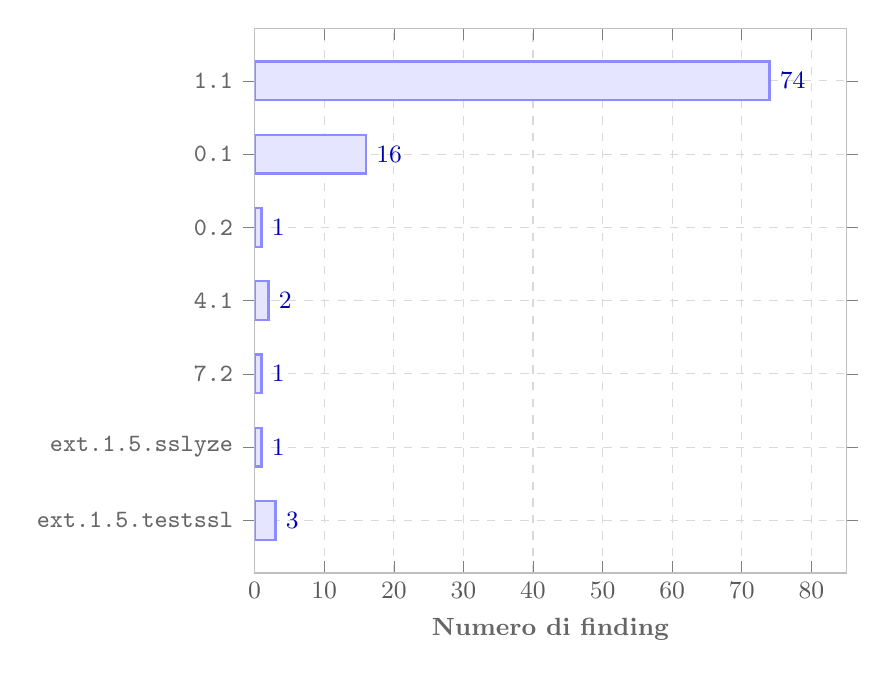
\begin{tikzpicture}
      \begin{axis}[
          xbar,
          width=0.75\textwidth, % <-- CORREZIONE: Lascia il 25% di spazio per le etichette laterali
          height=8.5cm,
          bar width=14pt,
          %
          % Setup Asse X
          xmin=0, xmax=85,
          xtick={0,10,20,30,40,50,60,70,80},
          xlabel={Numero di finding},
          xlabel style={font=\small\bfseries, text=gray!80!black},
          tick label style={font=\small, text=gray!70!black},
          %
          % Setup Asse Y
          symbolic y coords={{ext.1.5.testssl},{ext.1.5.sslyze},{7.2},{4.1},{0.2},{0.1},{1.1}},
          ytick=data,
          yticklabel style={font=\small\ttfamily, text=gray!80!black},
          enlarge y limits=0.12,
          %
          % Griglia
          grid=major,
          grid style={dashed, gray!30},
          axis line style={gray!50},
          %
          % Numeri a fianco delle barre
          nodes near coords,
          nodes near coords align={horizontal},
          every node near coord/.style={font=\small\bfseries, text=blue!70!black},
        ]

        \addplot[fill=blue!10, draw=blue!45, thick] coordinates {
            (3,{ext.1.5.testssl})
            (1,{ext.1.5.sslyze})
            (1,{7.2})
            (2,{4.1})
            (1,{0.2})
            (16,{0.1})
            (74,{1.1})
          };
      \end{axis}
    \end{tikzpicture}
  \end{adjustbox}
  \caption{Distribuzione dei 98 finding per test nell'assessment di validazione.}
  \label{fig:finding-distribution}
\end{figure}

\noindent{\small Cap.~5, §5.3, [DISCUTI] distribuzione 98 finding per test. Verificare ridondanza con tab:risultati-per-test.}
\clearpage

% ── Cap. 6 ───────────────────────────────────────────────────────────────────

% INSERIRE
% Cap. 6, §6.2.1
%
% PRIMA   : "Con codici semanticamente distinti questo routing è automatizzabile senza leggere i log."
% DOPO    : "Sistemi di \gls{CI/CD} come GitHub Actions o GitLab \gls{CI}"
% REF     : modifica frase esistente:
%   PRIMA "Con codici semanticamente distinti questo routing è automatizzabile senza leggere i log."
%   DOPO  "Con codici semanticamente distinti questo routing è automatizzabile senza leggere i log, come schematizzato nella Figura~\ref{fig:cicd-decision-tree}."
\begin{figure}[htbp]
  \centering
  \begin{adjustbox}{max width=\textwidth}
    \begin{tikzpicture}[
        % Stili Gold Standard (niente dipendenze da classi esterne)
        base/.style={draw, rounded corners=1pt, inner sep=6pt, align=center, font=\small, minimum height=3.5ex},
        cmd/.style={base, fill=blue!5, draw=blue!40, font=\small\ttfamily, minimum width=16em},
        decision/.style={draw, shape=diamond, aspect=2.5, inner sep=2pt, align=center, font=\small, fill=orange!10, draw=orange!50},
        %
        % Stili per gli Exit Codes (Larghezza fissa per allineamento a colonna)
        code0/.style={base, fill=green!10, draw=green!50!black, minimum width=8.5em},
        code1/.style={base, fill=red!10, draw=red!60!black, minimum width=8.5em},
        code2/.style={base, fill=orange!10, draw=orange!60!black, minimum width=8.5em},
        code10/.style={base, fill=gray!15, draw=gray!60!black, minimum width=8.5em},
        %
        % Stili per le Actions (Larghezza fissa e generosa)
        act0/.style={base, fill=green!5, draw=green!40, minimum width=13em},
        act1/.style={base, fill=red!5, draw=red!40, minimum width=13em},
        act2/.style={base, fill=orange!5, draw=orange!40, minimum width=13em},
        act10/.style={base, fill=gray!5, draw=gray!40, minimum width=13em},
      ]

      %% ── Asse Centrale (Runner -> Comando -> Decisione) ────────────────────
      \node[base, fill=gray!10, draw=gray!40, font=\small\bfseries] (start) {Runner CI/CD};
      \node[cmd, below=3ex of start] (cmd) {apiguard run -{}-config config.yaml};
      \node[decision, below=3ex of cmd] (dec) {exit code?};

      %% ── Colonna Exit Codes (Ancorati in alto a sx, coordinate forzate) ────
      % Il primo è spostato a destra di 4em rispetto al centro del rombo
      \path (dec.south) ++(4em, -4ex) node[code0, anchor=north west] (e0) {\textbf{\texttt{0}: CLEAN}\\{\scriptsize tutti PASS/SKIP}};
      \path (e0.south west) ++(0, -2.5ex) node[code1, anchor=north west] (e1) {\textbf{\texttt{1}: FAIL}\\{\scriptsize almeno un FAIL}};
      \path (e1.south west) ++(0, -2.5ex) node[code2, anchor=north west] (e2) {\textbf{\texttt{2}: ERROR}\\{\scriptsize ERROR senza FAIL}};
      \path (e2.south west) ++(0, -2.5ex) node[code10, anchor=north west] (e10) {\textbf{\texttt{10}: INFRA}\\{\scriptsize errore infrastrutturale}};

      %% ── Colonna Actions (Ancorate esattamente a 3em a destra dei codici) ──
      \path (e0.east) ++(3em, 0) node[act0, anchor=west] (a0) {\textbf{Pipeline prosegue}\\{\scriptsize (merge / deploy consentito)}};
      \path (e1.east) ++(3em, 0) node[act1, anchor=west] (a1) {\textbf{Blocco merge/deploy}\\{\scriptsize Report allegato come artefatto}};
      \path (e2.east) ++(3em, 0) node[act2, anchor=west] (a2) {\textbf{Alert malfunzionamento}\\{\scriptsize Revisione manuale richiesta}};
      \path (e10.east) ++(3em, 0) node[act10, anchor=west] (a10) {\textbf{Diagnosi deployment}\\{\scriptsize Verifica \texttt{config.yaml}}};

      %% ── Frecce di Flusso Principale ───────────────────────────────────────
      % Uso -latex per garantire la punta della freccia pulita senza dipendere da ag-arr
      \draw[-latex, semithick] (start) -- (cmd);
      \draw[-latex, semithick] (cmd) -- (dec);

      %% ── Routing a Bus per le condizioni (Il tronco verticale) ─────────────
      \coordinate (bus-end) at (dec.south |- e10.west);
      \draw[gray!70, semithick] (dec.south) -- (bus-end);

      % Diramazioni orizzontali verso gli Exit Code (colorate)
      \draw[-latex, semithick, green!50!black] (dec.south |- e0.west) -- (e0.west);
      \fill[gray!70] (dec.south |- e0.west) circle (1.5pt);

      \draw[-latex, semithick, red!60!black] (dec.south |- e1.west) -- (e1.west);
      \fill[gray!70] (dec.south |- e1.west) circle (1.5pt);

      \draw[-latex, semithick, orange!60!black] (dec.south |- e2.west) -- (e2.west);
      \fill[gray!70] (dec.south |- e2.west) circle (1.5pt);

      \draw[-latex, semithick, gray!60!black] (dec.south |- e10.west) -- (e10.west);
      \fill[gray!70] (dec.south |- e10.west) circle (1.5pt);

      %% ── Frecce dalle Condizioni alle Azioni (colorate in scala) ───────────
      \draw[-latex, semithick, green!50!black] (e0.east) -- (a0.west);
      \draw[-latex, semithick, red!60!black] (e1.east) -- (a1.west);
      \draw[-latex, semithick, orange!60!black] (e2.east) -- (a2.west);
      \draw[-latex, semithick, gray!60!black] (e10.east) -- (a10.west);

    \end{tikzpicture}
  \end{adjustbox}
  \caption{Routing degli exit code semantici (D6.P1) nella pipeline \gls{CI/CD}.}
  \label{fig:cicd-decision-tree}
\end{figure}

\noindent{\small Cap.~6, §6.2.1, routing exit code semantici (D6.P1): 0 clean, 1 fail, 2 error, 10 infra.}
\clearpage

% INSERIRE
% Cap. 6, §6.3.2
%
% PRIMA   : "garantendo che i finding prodotti da moduli distinti siano confrontabili nel report finale."
% DOPO    : "\paragraph{Coverage augmentation progressiva.}"
% REF     : aggiungere frase nel corpo del paragrafo prima della figura: La Figura~\ref{fig:modular-platform} illustra l'architettura a stella risultante, con il core invariato e i moduli di protocollo come unità intercambiabili.
\begin{figure}[htbp]
  \centering
  \begin{adjustbox}{max width=\textwidth}
    \begin{tikzpicture}[
        % Distanze calibrate
        node distance=4.5ex and 2.5em,
        %
        % Stili di base
        base/.style={draw, rounded corners=2pt, inner sep=8pt, align=center, font=\small},
        %
        % Core invariante leggermente allargato a 22em per accogliere la nuova riga dei contratti
        core/.style={base, fill=blue!8, draw=blue!45, minimum width=22em, thick},
        % Plugin mantenuto proporzionale (2em in meno del core)
        active/.style={base, fill=green!10, draw=green!50!black, minimum width=20em},
        %
        % Moduli Satelliti
        planned/.style={base, fill=gray!4, draw=gray!40, dashed, minimum width=8em},
        %
        % Stili Frecce
        arr-active/.style={-latex, thick, green!50!black},
        arr-planned/.style={-latex, thick, dashed, gray!50}
      ]

      %% ── Core immutabile (Centro) ──────────────────────────────────────────
      \node[core] (core) {
      \textbf{Core: infrastruttura immutabile}\\[1.5ex]
      {\footnotesize \texttt{Engine} \textbar{} \texttt{DAGScheduler} \textbar{} \texttt{EvidenceStore}}\\[0.8ex]
      {\footnotesize \texttt{TestContext} \textbar{} \texttt{TargetContext}}\\[0.8ex]
      {\footnotesize \texttt{BaseTest} \textbar{} \texttt{BaseConnector} \textbar{} \texttt{BaseGatewayAdapter}}\\[0.8ex]
      {\footnotesize \texttt{TestResult} \textbar{} \texttt{Finding} \textbar{} \texttt{EvidenceRecord}}
      };

      %% ── Moduli Satelliti (A stella) ───────────────────────────────────────
      % Modulo attivo (Sopra)
      \node[active, above=of core] (rest) {
      \textbf{Plugin REST (\gls{OAS})} \ {\footnotesize\itshape (attivo)}\\[1.5ex]
      {\footnotesize \texttt{OpenAPI discovery} \textbar{} \texttt{AttackSurface}}\\[0.8ex]
      {\footnotesize \texttt{SecurityClient} \textbar{} \texttt{KongGatewayAdapter}}\\[0.8ex]
      {\footnotesize 18 Test nativi (Domini D0--D7)}
      };

      % Moduli pianificati (Destra, Sotto, Sinistra)
      \node[planned, right=of core] (gql) {\textbf{GraphQL}\\[0.5ex]{\footnotesize\itshape (pianificato)}};
      \node[planned, below=of core] (grpc) {\textbf{gRPC}\\[0.5ex]{\footnotesize\itshape (pianificato)}};
      \node[planned, left=of core] (ws) {\textbf{WebSocket}\\[0.5ex]{\footnotesize\itshape (pianificato)}};

      %% ── Frecce di Collegamento (Convergenti verso il Core) ────────────────
      \draw[arr-active] (rest.south) -- (core.north);
      \draw[arr-planned] (gql.west) -- (core.east);
      \draw[arr-planned] (grpc.north) -- (core.south);
      \draw[arr-planned] (ws.east) -- (core.west);

      %% ── Legenda e Note ────────────────────────────────────────────────────
      \node[font=\footnotesize, text=gray!80!black, below=4ex of grpc, align=center] (note) {
      frecce continue: modulo attivo \quad frecce tratteggiate: moduli pianificati\\[1ex]
      {\itshape Il discovery dinamico via \texttt{pkgutil} permette il caricamento trasparente di moduli di terze parti}
      };

    \end{tikzpicture}
  \end{adjustbox}
  \caption{Evoluzione di APIGuard Assurance verso una piattaforma modulare: separazione netta tra il core invariante e i plugin di protocollo.}
  \label{fig:modular-platform}
\end{figure}
\noindent{\small Cap.~6, §6.3.2, piattaforma modulare: core immutabile + moduli REST/GraphQL/gRPC/WebSocket.}
\clearpage in main.tex (commentare prima della consegna).

\chapter{Asset test: figure e tabelle}

\makeatletter
\renewcommand{\fps@figure}{H}
\renewcommand{\fps@table}{H}
\makeatother

% ═══════════════════════════════════════════════════════════════════════════════
\section{Tabelle}
% ═══════════════════════════════════════════════════════════════════════════════

% ── Cap. 2 ───────────────────────────────────────────────────────────────────

% INSERIRE
% Cap. 2, §2.2.1
%
% PRIMA   : "Questa caratteristica impone vincoli specifici sulle tipologie di verifica applicabili in sede di assessment."
% DOPO    : "\subsection{Criteri di Selezione e Giustificazione Architetturale} \label{subsec:criteri-selezione}"
% REF     : aggiungere frase nuova prima della tabella: La Tabella~\ref{tab:modelli-esposizione} confronta i quattro modelli lungo le dimensioni rilevanti per il security assessment.
\begin{table}[ht]
  \centering \small
  \begin{tabularx}{\textwidth}{@{} p{3.0cm} p{1.8cm} X X X @{}}
    \toprule
    \textbf{Modello}
     & \textbf{Traffico presidiato}
     & \textbf{Enforcement policy}
     & \textbf{Accesso al piano di configurazione}
     & \textbf{Verifica \texttt{WHITE\_BOX}}           \\
    \midrule
    Gateway \gls{API} Dedicato (es.\ Kong, Apigee)
     & Nord-sud
     & Centralizzato in un unico strato ispezionabile
     & Admin \gls{API} diretta
     & Nativa                                          \\
    \addlinespace
    Kubernetes Ingress / Gateway \gls{API}
     & Nord-sud
     & Parziale: annotation controller-specifiche
     & \texttt{kubectl} / Kubernetes \gls{API}
     & Controller-dipendente                           \\
    \addlinespace
    Service Mesh (es.\ Istio)
     & Est-ovest
     & Distribuito per sidecar proxy
     & Control plane (istiod)
     & Fuori perimetro nord-sud                        \\
    \addlinespace
    Gateway Managed Cloud (AWS, Azure, GCP)
     & Nord-sud
     & Centralizzato: gestito interamente dal provider
     & \gls{SDK} / \gls{API} del cloud provider
     & Richiede adapter dedicato                       \\
    \bottomrule
  \end{tabularx}
  \caption{Confronto dei quattro modelli di esposizione in rete lungo le dimensioni rilevanti per il security assessment: il gateway \gls{API} dedicato è l'unico con Admin \gls{API} diretta e verifica \texttt{WHITE\_BOX} nativa.}
  \label{tab:modelli-esposizione}
\end{table}

\noindent{\small Cap.~2, §2.2.1, confronto modelli di esposizione: enforcement, accesso piano di configurazione, verificabilità WHITE\_BOX.}
\clearpage

% INSERIRE
% Cap. 2, §2.3.1
%
% PRIMA   : "richiesta sintatticamente corretta che viola le assunzioni del sistema sull'identità, i privilegi o il comportamento atteso del chiamante."
% DOPO    : "Colmare il semantic gap richiede che lo strumento disponga di una rappresentazione formale"
% REF     : modifica frase esistente:
%   PRIMA "...sono tutte vulnerabilità semantiche."
%   DOPO  "...sono tutte vulnerabilità semantiche, come sintetizzato nella Tabella~\ref{tab:semantic-gap}."
\begin{table}[ht]
  \centering \small
  \begin{tabularx}{\textwidth}{@{} l l C L @{}}
    \toprule
    \textbf{Vulnerabilità OWASP} & \textbf{Natura} & \textbf{Visibilità WAF/DAST} & \textbf{Prerequisito informativo} \\
    \midrule
    API1:2023: BOLA              & Semantica       & Cieca                        & Token $\geq 2$ ruoli              \\
    \addlinespace
    API2:2023: Broken Auth       & Sin./Sem.       & Parziale                     & Nessuno (BLACK\_BOX)              \\
    \addlinespace
    API3:2023: BOPLA             & Semantica       & Cieca                        & Token autenticato                 \\
    \addlinespace
    API5:2023: BFLA              & Semantica       & Cieca                        & Token $\geq 2$ ruoli              \\
    \addlinespace
    API7:2023: SSRF              & Semantica       & Parziale                     & Nessuno / token                   \\
    \bottomrule
  \end{tabularx}
  \caption{Tassonomia OWASP API Security Top~10 (2023): natura, visibilità WAF/DAST e prerequisito informativo per la rilevazione.}
  \label{tab:semantic-gap}
\end{table}
\noindent{\small Cap.~2, §2.3.1, tassonomia OWASP Top~10 (2023): natura, visibilità WAF/DAST, prerequisito informativo.}
\clearpage

% INSERIRE
% Cap. 2, §2.4.3
%
% PRIMA   : "i verdetti dipendono dalle proprietà definite dall'utente, non da un oracolo derivato dal contratto dell'endpoint."
% DOPO    : (fine del file)
% REF     : aggiungere frase nuova prima della tabella: La Tabella~\ref{tab:testing-comparison} sintetizza le differenze strutturali tra i paradigmi esaminati, riportando per ciascuno il tipo di conoscenza del contratto sfruttata, la disponibilità di un oracle formale e il livello di copertura semantica raggiungibile.
\begin{table}[ht]
  \centering \small
  \begin{tabularx}{\textwidth}{@{} l C C C C @{}}
    \toprule
    \textbf{Paradigma}                & \textbf{Conoscenza contratto} & \textbf{Oracle formale} & \textbf{Riproducibilità} & \textbf{Copertura semantica} \\
    \midrule
    SAST                              & Sorgente                      & Nessuno                 & Alta                     & Bassa                        \\
    \addlinespace
    DAST (ZAP)                        & Nessuna                       & Nessuno                 & Media                    & Bassa                        \\
    \addlinespace
    Fuzzer OAS (RESTler/Schemathesis) & Spec OAS                      & Parziale                & Media                    & Media                        \\
    \addlinespace
    \textbf{APIGuard Assurance}       & \textbf{Spec OAS + config}    & \textbf{OAS formale}    & \textbf{Alta}            & \textbf{Alta}                \\
    \bottomrule
  \end{tabularx}
  \caption{Confronto tra paradigmi di security testing per \gls{API} REST: oracle, riproducibilità e copertura semantica.}
  \label{tab:testing-comparison}
\end{table}

\noindent{\small Cap.~2, §2.4.3, confronto paradigmi: SAST, DAST, Fuzzer OAS, APIGuard (oracle, riproducibilità, copertura semantica).}
\clearpage

% ── Cap. 3 ───────────────────────────────────────────────────────────────────

% FATTO \cmark
% Cap. 3, introduzione capitolo
\begin{table}[ht]
  \centering
  \small
  % Abbandoniamo tabularx. Usiamo l l per il dominio e p{22em} per le proprietà.
  \begin{tabular}{@{} l l >{\raggedright\arraybackslash}p{22em} @{}}
    \toprule
    % Uniamo le prime due colonne solo per l'intestazione
    \multicolumn{2}{@{}l}{\textbf{Dominio}} & \textbf{Proprietà}                                                                                                                                                                                                                                                                                                                             \\
    \midrule
    \textbf{D1}                             & Architettura \& Design          &
    \hyperref[subsec:agnosticismo]{\textbf{D1.P1}}, \hyperref[subsec:dep-flow]{\textbf{D1.P2}}, \hyperref[subsec:split-state]{\textbf{D1.P3}}, \hyperref[subsec:dual-hierarchy]{D1.P4}, \hyperref[subsec:connector-hierarchy]{D1.P5}, \hyperref[subsec:gateway-adapter]{\textbf{D1.P6}}                                                                                                      \\
    \addlinespace
    \textbf{D2}                             & Estensibilità \& Manutenibilità &
    \hyperref[subsec:discovery-impl]{D2.P1}, \hyperref[subsec:dag]{\textbf{D2.P2}}, \hyperref[subsec:connector-hierarchy]{D2.P3}, \hyperref[subsec:connector-injection]{D2.P4}, \hyperref[subsec:auth-layer]{D2.P5}, \hyperref[subsec:connector-classification]{D2.P6}, \hyperref[subsec:path-seed]{D2.P7}, \hyperref[subsec:payload-catalog]{D2.P8}                                         \\
    \addlinespace
    \textbf{D3}                             & Config \& Riproducibilità       &
    \hyperref[subsec:config-driven]{\textbf{D3.P1}}, \hyperref[subsec:openapi-sot]{\textbf{D3.P2}}, \hyperref[subsec:box-gradient]{\textbf{D3.P3}}, \hyperref[subsec:reproducibility]{\textbf{D3.P4}}, \hyperref[subsec:zero-state]{\textbf{D3.P5}}                                                                                                                                          \\
    \addlinespace
    \textbf{D4}                             & Robustezza \& Sicurezza         &
    \hyperref[subsec:evidence-store]{\textbf{D4.P1}}, \hyperref[subsec:sanitization]{D4.P2}, \hyperref[subsec:fail-safe]{D4.P3}, \hyperref[subsec:exception-hierarchy]{D4.P4}, \hyperref[subsec:graceful-degradation]{D4.P5}, \hyperref[subsec:teardown]{D4.P6}, \hyperref[subsec:probing-policy]{D4.P7}, \hyperref[subsec:fail-fast]{D4.P8}, \hyperref[subsec:testresult-invariants]{D4.P9} \\
    \addlinespace
    \textbf{D5}                             & Qualità \& Osservabilità        &
    \hyperref[subsec:traceability]{D5.P1}, \hyperref[subsec:traceability]{D5.P2}, \hyperref[subsec:payload-catalog]{D5.P3}, D5.P4, \hyperref[subsec:dual-audit-trail]{D5.P5}                                                                                                                                                                                                                 \\
    \addlinespace
    \textbf{D6}                             & CI/CD \& DevEx                  &
    \hyperref[subsec:exit-codes]{D6.P1}, D6.P2, \hyperref[subsec:dual-layer-type-safety]{D6.P3}                                                                                                                                                                                                                                                                                              \\
    \addlinespace
    \textbf{D7}                             & Packaging \& Deployment         &
    \hyperref[subsec:connector-hierarchy]{D7.P1}, \hyperref[subsec:agpl-isolation]{D7.P2}, D7.P3                                                                                                                                                                                                                                                                                             \\
    \bottomrule
  \end{tabular}
  \caption{Proprietà APIGuard Assurance per dominio.}
  \label{tab:property-index}
\end{table}
\noindent{\small Cap.~3, intro, mappa delle 39 proprietà architetturali per dominio.}
\clearpage

% FATTO \cmark
% Cap. 3, §3.3.1
\begin{table}[ht]
  \centering
  \small
  % tabularx risolve l'equazione dello spazio: colonna c, colonna l, e il resto a X
  \begin{tabularx}{\textwidth}{@{} c l >{\raggedright\arraybackslash}X @{}}
    \toprule
    \textbf{Dominio} & \textbf{Titolo}                   & \textbf{Ambito di verifica}                                                                                                   \\
    \midrule
    D0               & API Discovery                     & Inventario degli endpoint esposti; rilevazione di Shadow API non documentate nella specifica.                                 \\
    \addlinespace
    D1               & Identity \& Authentication        & Meccanismi di riconoscimento del chiamante; robustezza del trasporto delle credenziali; ciclo di vita e revoca dei \gls{JWT}. \\
    \addlinespace
    D2               & Authorization                     & Logiche di controllo degli accessi; difetti di segregazione orizzontale e verticale (\gls{RBAC}, \gls{BOLA}).                 \\
    \addlinespace
    D3               & Data Integrity                    & Coerenza strutturale dei payload; implementazione delle firme crittografiche (\gls{HMAC}).                                    \\
    \addlinespace
    D4               & Availability \& Resilience        & Difese contro l'esaurimento delle risorse; audit di circuit breaker e soglie di rate limiting.                                \\
    \addlinespace
    D5               & Observability                     & Qualità e tempestività della telemetria generata dal sistema.                                                                 \\
    \addlinespace
    D6               & Configuration \& Hardening        & Rafforzamento della configurazione del gateway; policy di routing; header di sicurezza \gls{HTTP}.                            \\
    \addlinespace
    D7               & Business Logic \& Sensitive Flows & Falle semantiche complesse: elusione dei vincoli di processo, \gls{SSRF}, race condition su operazioni critiche.              \\
    \bottomrule
  \end{tabularx}
  \caption{Domini di Assurance di APIGuard Assurance.}
  \label{tab:domini}
\end{table}
\noindent{\small Cap.~3, §3.3.1, otto domini di assurance con titolo e ambito.}
\clearpage

% DISCUTI
% Cap. 3, §3.3.1
%
% Terza tabella nello stesso contesto di tab:domini e tab:box-gradient. Valutare se integrare le colonne Strategia e Implementato direttamente in tab:domini invece di aggiungere una tabella separata.
%
% PRIMA   : "Questa catena logica si riflette nelle dipendenze dichiarate dai singoli test che operano su questi domini, il cui meccanismo di risoluzione è descritto nella Sezione~\ref{subsec:dag}."
% DOPO    : "Domain-5 occupa una posizione particolare nella tassonomia: il dominio è architetturalmente predisposto"
% REF     : aggiungere frase prima della tabella: La Tabella~\ref{tab:domini-box-gradient} integra la vista precedente con la strategia operativa assegnata a ciascun dominio e lo stato di implementazione nella Milestone~1.
\begin{table}[ht]
  \centering \small
  \begin{tabularx}{\textwidth}{@{} l L C C C @{}}
    \toprule
    \textbf{Dominio}   & \textbf{Oggetto di verifica}          & \textbf{Strategia} & \textbf{Priorità} & \textbf{Implementato}  \\
    \midrule
    D0: Discovery      & Inventario endpoint, Shadow \gls{API} & BLACK/GREY         & P0--P1            & \cmark                 \\
    \addlinespace
    D1: Authentication & Autenticazione, lifecycle token       & BLACK/GREY         & P0--P1            & \cmark                 \\
    \addlinespace
    D2: Authorization  & \gls{RBAC}, \gls{BOLA}, \gls{BFLA}    & GREY               & P1--P2            & \cmark                 \\
    \addlinespace
    D3: Data Integrity & Schema, Mass Assignment               & GREY               & P2                & \cmark                 \\
    \addlinespace
    D4: Availability   & Rate limiting, circuit breaking       & GREY/WHITE         & P1--P2            & \cmark                 \\
    \addlinespace
    D5: Observability  & Log, tracing, audit trail             & WHITE              & P3                & \xmark{} (pianificato) \\
    \addlinespace
    D6: Hardening      & Security headers, config. gateway     & WHITE              & P2--P3            & \cmark                 \\
    \addlinespace
    D7: Business Logic & Flussi sensibili, \gls{SSRF}          & GREY               & P2                & \cmark                 \\
    \bottomrule
  \end{tabularx}
  \caption{Tassonomia degli otto domini di assurance: strategia di testing (Box Gradient D3.P3), priorità e stato implementativo nella versione corrente.}
  \label{tab:domini-box-gradient}
\end{table}

\noindent{\small Cap.~3, §3.3.1, [DISCUTI] domini con strategia Box Gradient e stato implementativo.}
\clearpage

% FATTO \cmark
% Cap. 3, §3.3.2
\begin{table}[ht]
  \centering
  \small
  % L'approccio ibrido perfetto: due colonne naturali e una dinamica a riempimento
  \begin{tabularx}{\textwidth}{@{} l l >{\raggedright\arraybackslash}X @{}}
    \toprule
    \textbf{Strategia}  & \textbf{Prerequisiti}               & \textbf{Razionale}                                                                                                             \\
    \midrule
    \texttt{BLACK\_BOX} & Nessuno (solo accesso di rete)      & Controlli perimetrali applicati dal gateway a qualsiasi interlocutore; simulazione di un attaccante esterno senza credenziali. \\
    \addlinespace
    \texttt{GREY\_BOX}  & Token per $\geq 2$ ruoli distinti   & Garanzie che presuppongono stato autenticato con identità di ruolo distinte; inaccessibili senza credenziali valide.           \\
    \addlinespace
    \texttt{WHITE\_BOX} & Accesso Admin \gls{API} del gateway & Configurazione statica verificabile per ispezione diretta tramite piano di controllo del gateway.                              \\
    \bottomrule
  \end{tabularx}
  \caption{Box Gradient applicato in APIGuard Assurance.}
  \label{tab:box-gradient}
\end{table}
\noindent{\small Cap.~3, §3.3.2, Box Gradient: precondizioni per strategia BLACK/GREY/WHITE.}
\clearpage

% ── Cap. 4 ───────────────────────────────────────────────────────────────────

% FATTO \cmark
% Cap. 4, §4.1
\begin{table}[ht]
  \centering
  \small
  \begin{tabular}{@{}lll@{}}
    \toprule
    \textbf{Fase}                 & \textbf{Cartella}               & \textbf{File}                         \\
    \midrule
    1. Inizializzazione           & \texttt{config/}                & \texttt{loader.py}                    \\
    \addlinespace
    2. OpenAPI Discovery          & \texttt{discovery/}             & \texttt{openapi.py}                   \\
    \addlinespace
    3. Costruzione Contesti       & \texttt{src/}                   & \texttt{engine.py}                    \\
    \addlinespace
    4. Test Discovery e \gls{DAG} & \texttt{tests/}, \texttt{core/} & \texttt{registry.py}, \texttt{dag.py} \\
    \addlinespace
    5. Esecuzione                 & \texttt{src/}                   & \texttt{engine.py}                    \\
    \addlinespace
    6. Teardown                   & \texttt{core/}                  & \texttt{context.py}                   \\
    \addlinespace
    7. Report                     & \texttt{report/}                & \texttt{renderer.py}                  \\
    \bottomrule
  \end{tabular}
  \caption{Fasi della pipeline di assessment (1-2-4 bloccanti; 5-6-7 non-bloccanti).}
  \label{tab:pipeline-fasi}
\end{table}

\noindent{\small Cap.~4, §4.1, fasi della pipeline con mapping cartella/file (1-2-4 bloccanti; 5-6-7 non-bloccanti).}
\clearpage

% FATTO \cmark
% Cap. 4, §4.1.2
%
% Nota: quando si inserisce fig:exception-hierarchy modificare anche la frase
% che introduce questa tabella nel capitolo:
%   PRIMA "...riportate nella Tabella~\ref{tab:exception-hierarchy} con la relativa fase."
%   DOPO  "...riportate nella Tabella~\ref{tab:exception-hierarchy} con la relativa fase, la cui struttura gerarchica è illustrata nella Figura~\ref{fig:exception-hierarchy}."
\begin{table}[ht]
  \centering
  \small
  \begin{tabularx}{\textwidth}{@{}llX@{}}
    \toprule
    \textbf{Classe}                   & \textbf{File}               & \textbf{Comportamento}                                                       \\
    \midrule
    \texttt{ToolBaseError}            & \texttt{exceptions.py}      & Radice della gerarchia; non si solleva direttamente                          \\
    \addlinespace
    \texttt{ConfigurationError}       & \texttt{exceptions.py}      & Fase~1: fatale, config non valida; blocca lo startup                         \\
    \addlinespace
    \texttt{OpenAPILoadError}         & \texttt{exceptions.py}      & Fase~2: fatale, spec irraggiungibile o invalida; blocca lo startup           \\
    \addlinespace
    \texttt{DAGCycleError}            & \texttt{exceptions.py}      & Fase~4: fatale, ciclo nelle dipendenze; blocca lo startup                    \\
    \addlinespace
    \texttt{AuthenticationSetupError} & \texttt{exceptions.py}      & Helper auth: fatale se le credenziali configurate sono invalide              \\
    \addlinespace
    \texttt{SecurityClientError}      & \texttt{exceptions.py}      & Fase~5: recuperata, produce \texttt{TestResult(ERROR)}                       \\
    \addlinespace
    \texttt{ExternalToolError}        & \texttt{exceptions.py}      & Fase~5: recuperata, produce \texttt{TestResult(ERROR)}                       \\
    \addlinespace
    \texttt{TeardownError}            & \texttt{exceptions.py}      & Fase~6: recuperata, registrata come \texttt{WARNING}                         \\
    \addlinespace
    \texttt{GatewayAdapterError}      & \texttt{gateway/base.py}    & Fase~5: recuperata, produce \texttt{TestResult(ERROR)}                       \\
    \addlinespace
    \texttt{SeedGeneratorFetchError}  & \texttt{seed\_generator.py} & \gls{CLI} \texttt{generate-seed}: catturata in \texttt{cli.py}, exit~code~10 \\
    \addlinespace
    \texttt{SeedGeneratorParseError}  & \texttt{seed\_generator.py} & \gls{CLI} \texttt{generate-seed}: catturata in \texttt{cli.py}, exit~code~10 \\
    \bottomrule
  \end{tabularx}
  \caption{Gerarchia delle eccezioni custom (Fasi 1--4 bloccanti; Fasi 5--6 recuperate localmente).}
  \label{tab:exception-hierarchy}
\end{table}

\noindent{\small Cap.~4, §4.1.2 11, eccezioni custom: file e comportamento (bloccanti Fasi~1--4; recuperate Fasi~5--6).}
\clearpage

% ── Cap. 5 ───────────────────────────────────────────────────────────────────

% FATTO \cmark
% Cap. 5, §5.1.1
\begin{table}[ht]
  \centering
  \small
  % Aggiunti i margini invisibili @{} e il raggedright per la colonna X
  \begin{tabularx}{\textwidth}{@{} l l >{\raggedright\arraybackslash}X @{}}
    \toprule
    \textbf{Componente}         & \textbf{Versione}     & \textbf{Ruolo nel testbed}                                                                                  \\
    \midrule
    \texttt{apiguard-assurance} & 0.1.0                 & Tool sotto validazione                                                                                      \\
    \addlinespace
    Python                      & 3.12.3                & Interprete del tool                                                                                         \\
    \addlinespace
    Forgejo                     & 14.0.3 (gitea-1.22.0) & Target applicativo: \gls{API} REST con specifica OpenAPI nativa                                             \\
    \addlinespace
    PostgreSQL                  & 15-alpine             & Backend di persistenza di Forgejo (dipendenza funzionale, non componente autonomo)                          \\
    \addlinespace
    Kong                        & 3.9 DB-less           & \gls{API} Gateway: proxy \gls{HTTP}/\gls{HTTPS}, instradamento verso Forgejo, Admin \gls{API} su porta 8001 \\
    \addlinespace
    \texttt{nuclei}             & 3.8.0                 & Tool esterno per Shadow \gls{API} discovery (test \texttt{ext.0.1})                                         \\
    \addlinespace
    \texttt{nuclei-templates}   & 10.4.3                & Base di template di scansione versioned: garantisce che lo stesso set di firme venga usato in ogni run      \\
    \addlinespace
    \texttt{testssl.sh}         & 3.2.3                 & Analisi \gls{TLS} black-box (test \texttt{ext.1.5.testssl})                                                 \\
    \addlinespace
    \texttt{sslyze}             & (libreria Python)     & Analisi \gls{TLS} via libreria Python (test \texttt{ext.1.5.sslyze})                                        \\
    \bottomrule
  \end{tabularx}
  \caption{Componenti e versioni dell'ambiente di test.}
  \label{tab:versioni-testbed}
\end{table}
\noindent{\small Cap.~5, §5.1.1, componenti e versioni dell'ambiente di test.}
\clearpage

% FATTO \cmark
% Cap. 5, §5.2.1
\begin{table}[ht]
  \centering
  \small
  \begin{tabularx}{\textwidth}{l l X}
    \toprule
    \textbf{Tool}      & \textbf{Esito}               & \textbf{Note}         \\
    \midrule
    \texttt{ruff}      & 0 errori                     &
    Ruleset \texttt{E/W/F/I/N/UP/B/S/ANN}                                     \\
    \addlinespace
    \texttt{mypy}      & 0 errori                     &
    Modalità \texttt{strict}: \texttt{no-implicit-optional},
    \texttt{disallow-untyped-defs}, \texttt{warn-return-any}                  \\
    \addlinespace
    \texttt{bandit}    & 0 finding severity medium$+$ &
    3 Low (B404, S603$\times$2) soppressi con \texttt{\#~noqa} documentati:
    invocazione subprocess controllata per design                             \\
    \addlinespace
    \texttt{vulture}   & 0 finding                    &
    Confidence $\ge$80\%; metodi a dispatching dinamico esclusi via whitelist \\
    \addlinespace
    \texttt{pip-audit} & 0 \gls{CVE}                  &
    Nessuna vulnerabilità nota nelle dipendenze dichiarate                    \\
    \bottomrule
  \end{tabularx}
  \caption{Risultati dell'analisi statica su APIGuard Assurance v0.1.0.}
  \label{tab:analisi-statica}
\end{table}

\noindent{\small Cap.~5, §5.2.1, risultati analisi statica v0.1.0 (ruff, mypy, bandit, vulture, pip-audit).}
\clearpage

% FATTO \cmark
% Cap. 5, §5.2.3
\begin{table}[ht]
  \centering
  \small
  \begin{tabularx}{\textwidth}{l l X}
    \toprule
    \textbf{Aspetto}            & \textbf{Stato} & \textbf{Dettaglio}                                                  \\
    \midrule
    Analisi statica             & \checkmark     &
    0 errori su tutti e cinque gli strumenti (Sezione~\ref{subsec:static-analysis})                                    \\
    \addlinespace
    Type safety                 & \checkmark     &
    0 errori mypy strict; validazione Pydantic attiva su tutti i confini (Sezione~\ref{subsec:dual-layer-type-safety}) \\
    \addlinespace
    Documentazione interna      & \checkmark     &
    292/292 simboli pubblici con docstring (100\%)                                                                     \\
    \addlinespace
    Riproducibilità della build & \checkmark     &
    SHA-256 identico su due build consecutive (451\,261~byte)                                                          \\
    \addlinespace
    Portabilità                 & \checkmark     &
    Cold install in ambiente pulito: \texttt{apiguard version} $\to$ \texttt{0.1.0}                                    \\
    \bottomrule
  \end{tabularx}
  \caption{Sintesi delle verifiche di qualità sulla codebase.}
  \label{tab:verdetto-release}
\end{table}

\noindent{\small Cap.~5, §5.2.3, sintesi verifiche qualità codebase.}
\clearpage

% FATTO \cmark
% Cap. 5, §5.3
\begin{table}[ht]
  \centering
  \small
  \begin{tabularx}{0.85\textwidth}{l C C C}
    \toprule
    \textbf{\gls{KPI}}                     & \textbf{Run~1}    & \textbf{Run~2}    & \textbf{$\Delta$} \\
    \midrule
    PASS / FAIL / SKIP / ERROR             & 9 / 7 / 2 / 0     & 9 / 7 / 2 / 0     & identico          \\
    \addlinespace
    Finding count totale                   & 98                & 98                & identico          \\
    \addlinespace
    \texttt{pass\_rate\_pct}               & 56.2\%            & 56.2\%            & identico          \\
    \addlinespace
    \texttt{assessment\_duration\_seconds} & 290.14\,s         & 290.81\,s         & $+$0.23\%         \\
    \addlinespace
    Exit code / label                      & 1 / \texttt{FAIL} & 1 / \texttt{FAIL} & identico          \\
    \bottomrule
  \end{tabularx}
  \caption{KPI di idempotenza su due run indipendenti.}
  \label{tab:idempotenza-kpi}
\end{table}

\noindent{\small Cap.~5, §5.3, KPI idempotenza su due run indipendenti.}
\clearpage

% FATTO \cmark
% Cap. 5, §5.3
\begin{table}[ht]
  \centering
  \small
  % Tabular puro con margini di 0.5em. Allineamenti: left, left, center, center, center
  \begin{tabular}{@{\hspace{0.5em}} l l c c c @{\hspace{0.5em}}}
    \toprule
    \textbf{Test ID}         & \textbf{Dominio}   & \textbf{Tipo} & \textbf{Status} & \textbf{Finding} \\
    \midrule
    \texttt{0.1}             & D0: Discovery      & Nativo        & \texttt{FAIL}   & 16               \\
    \texttt{0.2}             & D0: Discovery      & Nativo        & \texttt{FAIL}   & 1                \\
    \texttt{0.3}             & D0: Discovery      & Nativo        & \texttt{SKIP}   & 0                \\
    \addlinespace
    \texttt{1.1}             & D1: Auth           & Nativo        & \texttt{FAIL}   & 74               \\
    \texttt{1.4}             & D1: Auth           & Nativo        & \texttt{PASS}   & 0                \\
    \texttt{1.5}             & D1: Auth           & Nativo        & \texttt{PASS}   & 0                \\
    \texttt{1.6}             & D1: Auth           & Nativo        & \texttt{SKIP}   & 0                \\
    \addlinespace
    \texttt{2.1}             & D2: Authorization  & Nativo        & \texttt{PASS}   & 0                \\
    \addlinespace
    \texttt{3.3}             & D3: Data Integrity & Nativo        & \texttt{PASS}   & 0                \\
    \addlinespace
    \texttt{4.1}             & D4: Availability   & Nativo        & \texttt{FAIL}   & 2                \\
    \texttt{4.2}             & D4: Availability   & Nativo        & \texttt{PASS}   & 0                \\
    \texttt{4.3}             & D4: Availability   & Nativo        & \texttt{PASS}   & 0                \\
    \addlinespace
    \texttt{6.2}             & D6: Hardening      & Nativo        & \texttt{PASS}   & 0                \\
    \texttt{6.4}             & D6: Hardening      & Nativo        & \texttt{PASS}   & 0                \\
    \addlinespace
    \texttt{7.2}             & D7: Business Logic & Nativo        & \texttt{FAIL}   & 1                \\
    \addlinespace
    \texttt{ext.0.1.nuclei}  & D0: Discovery      & Esterno       & \texttt{PASS}   & 0                \\
    \texttt{ext.1.5.sslyze}  & D1: Auth           & Esterno       & \texttt{FAIL}   & 1                \\
    \texttt{ext.1.5.testssl} & D1: Auth           & Esterno       & \texttt{FAIL}   & 3                \\
    \midrule
    \textbf{Totale}          &                    &               &                 & \textbf{98}      \\
    \bottomrule
  \end{tabular}
  \caption{Status e finding count per test.}
  \label{tab:risultati-per-test}
\end{table}
\noindent{\small Cap.~5, §5.3, status e finding count per ciascuno dei 18 test.}
\clearpage

% FATTO \cmark
% Cap. 5, §5.4
\begin{table}[ht]
  \centering
  \small
  \begin{tabularx}{\textwidth}{l C C}
    \toprule
    \textbf{Metrica}       & \textbf{Run~1}      & \textbf{Run~2}      \\
    \midrule
    Wall-clock elapsed     & 290.14\,s (4:50.14) & 290.81\,s (4:50.81) \\
    \addlinespace
    User time              & 35.09\,s            & 34.67\,s            \\
    \addlinespace
    System time            & 41.51\,s            & 41.62\,s            \\
    \addlinespace
    Peak resident set size & 287\,MB             & 295\,MB             \\
    \bottomrule
  \end{tabularx}
  \caption{Metriche di sistema sui due run.}
  \label{tab:performance-baseline}
\end{table}

\noindent{\small Cap.~5, §5.4, metriche di sistema sui due run (wall-clock, CPU, memoria).}
\clearpage

% FATTO \cmark
% Cap. 5, §5.4.2
\begin{table}[ht]
  \centering
  \small
  % tabularx per mandare a capo i test.
  % Cardinalità centrata (c) e allineamento a bandiera (raggedright) per evitare spazi dilatati
  \begin{tabularx}{\textwidth}{@{\hspace{0.5em}} l c >{\raggedright\arraybackslash}X @{\hspace{0.5em}}}
    \toprule
    \textbf{Fase DAG}                        & \textbf{Cardinalità} & \textbf{Test}                                                                                                                                                                                                                                                                                           \\
    \midrule
    Phase~A (nessuna dipendenza)             & 16 test              &
    \texttt{0.1} $\cdot$ \texttt{0.2} $\cdot$ \texttt{0.3} $\cdot$ \texttt{1.1} $\cdot$ \texttt{1.5} $\cdot$ \texttt{1.6} $\cdot$ \texttt{3.3} $\cdot$ \texttt{4.1} $\cdot$ \texttt{4.2} $\cdot$ \texttt{4.3} $\cdot$ \texttt{6.2} $\cdot$ \texttt{6.4} $\cdot$ \texttt{7.2} $\cdot$ \texttt{ext.0.1.nuclei} $\cdot$ \texttt{ext.1.5.testssl} $\cdot$ \texttt{ext.1.5.sslyze} \\
    \addlinespace
    Phase~B (\texttt{depends\_on = ["1.1"]}) & 2 test               &
    \texttt{1.4} $\cdot$ \texttt{2.1}                                                                                                                                                                                                                                                                                                                                         \\
    \bottomrule
  \end{tabularx}
  \caption{Topologia del \gls{DAG} nell'assessment di validazione.}
  \label{tab:dag-topology}
\end{table}
\noindent{\small Cap.~5, §5.4.2, topologia DAG: Phase~A (16 test) e Phase~B (\texttt{depends\_on=["1.1"]}).}
\clearpage

% ═══════════════════════════════════════════════════════════════════════════════
\section{Figure}
% ═══════════════════════════════════════════════════════════════════════════════

% ── Cap. 2 ───────────────────────────────────────────────────────────────────

% INSERIRE
% Cap. 2, §2.4.1
%
% PRIMA   : "questo è il limite strutturale del fuzzing cieco applicato alle \gls{API} REST~\cite{MISSING:atlidakis:2019:restler}."
% DOPO    : "Quando invece il contratto è disponibile, la \gls{OAS} diventa la prima e più precisa fonte di conoscenza:"
% REF     : modifica frase esistente:
%   PRIMA "...il limite strutturale del fuzzing cieco applicato alle \gls{API} REST~\cite{MISSING:atlidakis:2019:restler}."
%   DOPO  "...il limite strutturale del fuzzing cieco applicato alle \gls{API} REST~\cite{MISSING:atlidakis:2019:restler}, illustrato schematicamente nella Figura~\ref{fig:combinatorial-wall}."
% ─── FIGURA B (8.1) -- Il Combinatorial Wall ─────────────────────────────────
\begin{figure}[htbp]
  \centering
  \begin{adjustbox}{max width=\textwidth}
    \begin{tikzpicture}[
        % Distanza orizzontale ridotta drasticamente per compattare
        node distance=4ex and 1em,
        %
        % STILE BASE: inner sep ridotto per non sprecare millimetri preziosi
        base/.style={draw, rounded corners=1.5pt, inner sep=3pt, align=center, font=\footnotesize, minimum height=3em},
        %
        % Larghezza colonna 1 ridotta al minimo indispensabile
        col1/.style={minimum width=7.5em},
        %
        % Stili per Via A
        viaA/.style={base, fill=red!6, draw=red!50},
        invis/.style={base, fill=gray!6, draw=gray!40, dashed, text=gray!70!black},
        %
        % Stili per Via B
        viaB/.style={base, fill=green!7, draw=green!45},
        vis/.style={base, fill=green!7, draw=green!50!black},
        %
        lbl/.style={font=\footnotesize\bfseries, inner sep=1pt},
        %
        arrA/.style={-latex, semithick, red!60!black},
        arrB/.style={-latex, semithick, green!50!black},
        arr-wall/.style={-latex, semithick, dashed, gray!60},
        %
        note/.style={font=\scriptsize\itshape, text=gray!70!black, align=center, inner sep=1.5pt}
      ]

      %% ── Via A ─────────────────────────────────────────────────────────────
      \node[viaA, col1] (a1) {Fuzzer\\sintattico};
      % Testo forzato su più righe stringendo il text width
      \node[viaA, right=of a1, text width=6.5em] (a2) {Payload casuali\\malformati};
      \node[viaA, right=of a2, text width=6.5em] (a3) {\texttt{400 Bad}\\\texttt{Request}};

      % Muro combinatorio ridotto a soli 3.5em
      \node[invis, right=3.5em of a3, text width=7em] (a4) {Logica\\applicativa\\{\scriptsize [invisibile]}};

      %% ── Via B ─────────────────────────────────────────────────────────────
      \node[viaB, col1, below=6ex of a1] (b1) {Engine\\contract-driven};

      \node[viaB] (b2) at (a2 |- b1) {Payload validi\\dalla spec \gls{OAS}};
      \node[viaB] (b3) at (a3 |- b1) {\texttt{2xx} / \texttt{4xx}\\semantici};
      \node[vis]  (b4) at (a4 |- b1) {Logica\\applicativa\\{\scriptsize [visibile]}};

      %% ── Etichette di corsia ────────────────────────────────────────────────
      % Distanza minima per recuperare spazio sul margine sinistro estremo
      \node[lbl, text=red!70!black, left=1em of a1] (lblA) {Via~A};
      \node[lbl, text=green!60!black] (lblB) at (lblA |- b1) {Via~B};

      %% ── Frecce Via A ───────────────────────────────────────────────────────
      \draw[arrA] (a1) -- (a2);
      \draw[arrA] (a2) -- (a3);
      % Scritta spostata SOTTO e abbassata leggermente con yshift
      \draw[arr-wall] (a3) -- node[midway, below, yshift=-0.5ex, note] {muro\\combinatorio} (a4);

      %% ── Frecce Via B ───────────────────────────────────────────────────────
      \draw[arrB] (b1) -- (b2);
      \draw[arrB] (b2) -- (b3);
      \draw[arrB] (b3) -- (b4);

      %% ── Linea di Separazione ───────────────────────────────────────────────
      \path (a1.south) ++(0, -3ex) coordinate (mid-y);
      \draw[gray!40, dashed, thick] ([xshift=-0.5em]lblA.west |- mid-y) -- ([xshift=0.5em]a4.east |- mid-y);

    \end{tikzpicture}%
  \end{adjustbox}
  \caption{Il \emph{combinatorial wall}: fuzzer sintattico (Via~A) vs.\ approccio contract-driven \gls{OAS} (Via~B).}
  \label{fig:combinatorial-wall}
\end{figure}
\noindent{\small Cap.~2, §2.4.1, combinatorial wall: fuzzer sintattico (Via~A) vs.\ engine contract-driven OAS (Via~B).}
\clearpage

% ── Cap. 3 ───────────────────────────────────────────────────────────────────

% INSERIRE
% Cap. 3, §3.2
%
% PRIMA   : "Le proprietà discusse nella sezione precedente costituiscono la base del sistema. Le scelte di questa sezione si aggiungono ad esse, ciascuna rispondendo a un'esigenza architetturale specifica che le proprietà fondamentali lasciano aperta."
% DOPO    : "\subsection{Flusso di Dipendenze Monodirezionale (D1.P2)} \label{subsec:dep-flow}"
% REF     : modifica prima frase di sec:architettura:
%   PRIMA "Le proprietà discusse nella sezione precedente costituiscono la base del sistema."
%   DOPO  "Le proprietà discusse nella sezione precedente costituiscono la base del sistema, i cui componenti principali e le loro relazioni sono illustrati nella Figura~\ref{fig:architettura-apiguard}."
\begin{figure}[ht]
  \centering
  % NIENTE \resizebox: il diagramma è ottimizzato per rientrare nella pagina
  % garantendo che i font \footnotesize vengano stampati alla loro vera grandezza.
  \begin{tikzpicture}[
      node distance=1.5ex and 2.5em,
      %
      % Stili di base Gold Standard
      base/.style={draw, rounded corners=1.5pt, inner sep=5pt, align=center, font=\small},
      %
      % Colonne snellite e uniformate (minimum height=3em per i blocchi principali)
      col-in/.style={base, fill=gray!10, draw=gray!50, minimum width=10em},
      col-mid-blue/.style={base, fill=blue!7, draw=blue!40, minimum width=14em, minimum height=3em},
      col-mid-green/.style={base, fill=green!7, draw=green!45, minimum width=14em, minimum height=3em},
      col-mid-gold/.style={base, fill=orange!10, draw=orange!50, minimum width=14em, minimum height=2.5em},
      col-mid-violet/.style={base, fill=violet!7, draw=violet!40, minimum width=14em, minimum height=3em},
      col-out/.style={base, fill=gray!8, draw=gray!50, minimum width=9.5em},
      %
      % Frecce ortogonali pulite
      arr/.style={-latex, semithick, gray!80!black},
      darr/.style={-latex, semithick, dashed, gray!80!black},
      barr/.style={latex-latex, semithick, gray!80!black},
      %
      % Etichette sulle frecce
      lbl/.style={font=\footnotesize\itshape, text=gray!70!black, inner sep=3pt},
      %
      % Sfondo per raggruppamento dinamico
      bg-engine/.style={draw=blue!30, fill=blue!3, dashed, rounded corners=3pt, inner sep=10pt}
    ]

    %% ── Engine (Colonna Centrale) Fissato per primo ──────────────────────
    % Altezza normalizzata tramite lo stile col-mid-blue
    \node[col-mid-blue] (tc) {\textbf{\texttt{TargetContext}} {\footnotesize[frozen]}\\{\footnotesize base\_url | attack\_surface | creds}};

    \node[col-mid-green, below=of tc] (tx) {\textbf{\texttt{TestContext}} {\footnotesize[mutable]}\\{\footnotesize token | teardown | shared\_data}};
    \node[col-mid-gold, below=of tx] (dag) {\textbf{DAG Scheduler}\\{\footnotesize ordinamento, batch sequenziali}};

    %% Box di raggruppamento dinamico (Assessment Engine)
    \begin{scope}[on background layer]
      \node[bg-engine, fit=(tc)(tx)(dag)] (engine) {};
    \end{scope}

    % Etichetta agganciata in alto a sinistra
    \node[font=\footnotesize\bfseries, text=blue!70!black, anchor=south east, shift={(-1em, 0.5ex)}]
    at (engine.north) {Assessment Engine};

    %% ── Input (Colonna Sinistra) Ancorati matematicamente ────────────────
    % Config.yaml: Allineato esattamente col tetto dell'engine (che ora si è abbassato proporzionalmente)
    \node[col-in, anchor=north east] (cfg) at ([xshift=-2.5em]tc.west |- engine.north) {\textbf{\texttt{config.yaml}}\\{\footnotesize credenziali, URL, param.}};

    % OpenAPI.yaml: Più in basso
    \node[col-in, anchor=east] (oas) at ([xshift=-2.5em, yshift=-7ex]tc.west) {\textbf{\texttt{openapi.yaml}}\\{\footnotesize spec formale target}};

    %% ── Target (Colonna Destra) ────────────────────────────────────────────
    \node[col-out, right=6em of tc] (kong) {\textbf{Kong Gateway}\\{\footnotesize :8000 / :8443 / :8001}};

    % Forgejo abbassato ulteriormente (8.5ex) per fare molto spazio all'etichetta Admin API
    \node[col-out, below=8.5ex of kong] (forgejo) {\textbf{Forgejo}\\{\footnotesize target applicativo}};

    %% ── EvidenceStore (Sotto l'Engine) ─────────────────────────────────────
    \node[col-mid-violet, below=4ex of dag] (ev) {\textbf{EvidenceStore} {\footnotesize[JSONL]}\\{\footnotesize \texttt{evidence.json} | \texttt{report.html}}};

    %% ── FRECCE E COLLEGAMENTI ──────────────────────────────────────────────

    %% Input -> Engine
    % config.yaml: Nessuna curva. Va dritto al TargetContext.
    \draw[arr] (cfg.east) -- (tc.west |- cfg.east);

    % openapi.yaml: Esce dall'alto, sale e curva entrando nella metà inferiore del TargetContext (-2ex)
    \draw[arr] (oas.north) |- ([yshift=-2ex]tc.west);

    %% Engine -> Target (Probe HTTP su due righe)
    \path (tc.east) ++(0, 1.5ex) coordinate (probe-start);
    \path (kong.west) ++(0, 1.5ex) coordinate (probe-end);
    \draw[arr] (probe-start) -- node[midway, above, align=center, lbl] {probe\\\gls{HTTP}} (probe-end);

    \draw[barr] (kong.south) -- (forgejo.north);

    %% Interne Engine -> Evidence
    \draw[arr] (dag.north) -- (tx.south);
    \draw[arr] (dag.south) -- (ev.north);

    %% Engine -> Target (Admin API - WHITE_BOX)
    \path (tx.east) ++(0, -1ex) coordinate (admin-start);
    \path (kong.west) ++(0, -1.5ex) coordinate (admin-end);

    % Punto di svolta inferiore (a 2.5em da TestContext)
    \path (admin-start) ++(2.5em, 0) coordinate (admin-turn1);

    % Punto di svolta superiore (l'angolo a 90° prima di entrare in Kong)
    \coordinate (admin-turn2) at (admin-turn1 |- admin-end);

    % Freccia strutturale pulita
    \draw[darr] (admin-start) -- (admin-turn1) -- (admin-turn2) -- (admin-end);

    % Etichetta posizionata incastonata nello spazio vuoto.
    % Spostata più in basso (yshift=-2ex) e leggermente più a sinistra (xshift=0.2em)
    \node[lbl, align=left, anchor=north west]
    at ([xshift=0.2em, yshift=-2ex]admin-turn2)
    {Admin \gls{API}\\{\footnotesize WHITE\_BOX}};

  \end{tikzpicture}
  \caption{Architettura di APIGuard Assurance: Engine, DAG Scheduler ed EvidenceStore.}
  \label{fig:architettura-apiguard}
\end{figure}

\noindent{\small Cap.~3, §3.2, architettura alto livello: input, Engine (Split State D1.P3), DAG Scheduler (D2.P2), EvidenceStore (D4.P1).}
\clearpage

% INSERIRE
% Cap. 3, §3.2.2
%
% PRIMA   : "Salvaguardia contro lo stallo: se il grafo risulta ancora attivo ma non riesce a estrarre nessun test pronto, il sistema emette un errore strutturato che elenca i test mai schedulati e interrompe l'esecuzione in modo controllato, fornendo all'operatore la diagnostica necessaria senza dover ricostruire lo stato interno del grafo."
% DOPO    : "L'ordinamento topologico puro non garantisce un ordine unico tra test pronti allo stesso livello:"
% REF     : aggiungere frase nuova dopo la chiusura del blocco itemize: La topologia del \gls{DAG} nell'assessment di validazione, con le due fasi di esecuzione risultanti, è illustrata nella Figura~\ref{fig:dag-topology}.
\begin{figure}[ht]
  \centering
  % NIENTE \resizebox: il diagramma usa font \footnotesize integrati e spazi 
  % calibrati per rientrare perfettamente nei margini mantenendo i testi nitidi.
  \begin{tikzpicture}[
      node distance=1.5ex and 1em,
      %
      % Stili dei Nodi (indipendenti dal preambolo)
      tst/.style={draw=orange!55, fill=yellow!18, rounded corners=1.5pt, minimum width=4.5em, minimum height=3.5ex, font=\footnotesize\ttfamily, align=center},
      tst-hl/.style={tst, draw=orange!70, fill=yellow!35, thick},
      ext/.style={tst, minimum width=6.5em, font=\scriptsize\ttfamily},
      %
      phB/.style={draw=blue!40, fill=blue!7, rounded corners=1.5pt, minimum width=5.5em, minimum height=3.5ex, font=\footnotesize\ttfamily, align=center},
      phC/.style={draw=gray!40, fill=gray!8, dashed, rounded corners=1.5pt, minimum width=7em, minimum height=4.5ex, font=\footnotesize, align=center},
      %
      % Stili dei Riquadri di Sfondo
      bg-A/.style={draw=orange!50, fill=yellow!6, dashed, rounded corners=3pt, inner sep=12pt},
      bg-B/.style={draw=blue!40, fill=blue!4, dashed, rounded corners=3pt, inner sep=10pt},
      %
      % Frecce native
      arr/.style={-latex, semithick, blue!60},
      darr/.style={-latex, semithick, dashed, gray!60}
    ]

    %% ── Phase A: 16 test (Griglia compatta) ───────────────────────────────
    % D0
    \node[tst] (d0a) {0.1};
    \node[tst, right=of d0a] (d0b) {0.2};
    \node[tst, right=of d0b] (d0c) {0.3};

    % D1 (ORDINE CORRETTO: 1.1 evidenziato a sinistra)
    \node[tst-hl, below=of d0a] (a11) {\textbf{1.1}};
    \node[tst, right=of a11] (d1b) {1.5};
    \node[tst, right=of d1b] (d1c) {1.6};

    % D3 (Gap maggiorato a 3.5ex per creare un "tunnel" orizzontale)
    \node[tst, below=3.5ex of a11] (d3a) {3.3};

    % D4
    \node[tst, below=of d3a] (d4a) {4.1};
    \node[tst, right=of d4a] (d4b) {4.2};
    \node[tst, right=of d4b] (d4c) {4.3};

    % D6
    \node[tst, below=of d4a] (d6a) {6.2};
    \node[tst, right=of d6a] (d6b) {6.4};

    % D7
    \node[tst, below=of d6a] (d7a) {7.2};

    % External tests: MANDATI A CAPO per contenere la larghezza totale di Phase A
    \node[ext, below=of d7a.south west, anchor=north west] (ex0) {ext.0.1.nuclei};
    \node[ext, below=of ex0.south west, anchor=north west] (ex1) {ext.1.5.sslyze};
    \node[ext, right=of ex1] (ex2) {ext.1.5.testssl};

    %% Box Phase A (Includiamo d1c per garantire che abbracci l'estrema destra)
    \begin{scope}[on background layer]
      \node[bg-A, fit=(d0a)(d0c)(a11)(d1c)(d7a)(ex1)(ex2)] (phaseA) {};
    \end{scope}

    % Etichetta Phase A ancorata sopra senza toccare il tratteggio
    \node[font=\footnotesize\bfseries, text=orange!80!black, anchor=south west]
    at ([xshift=1ex, yshift=0.5ex]phaseA.north west) {Phase A (16 test, nessuna dipendenza)};

    %% ── Snodo e Phase B (Biforcazione Simmetrica Esterna) ─────────────────
    % 1. Calcolo del tunnel: scendiamo a metà esatta del gap (1.75ex sotto a 1.1)
    \path (a11.south) ++(0, -1.75ex) coordinate (bus-y);

    % 2. Punto di uscita dal box giallo
    \path (phaseA.east |- bus-y) coordinate (exitA);

    % 3. Snodo matematico: 3.5em di distanza a destra del box giallo
    \path (exitA) ++(3.5em, 0) coordinate (split);

    % I due test di Phase B allineati verticalmente allo snodo
    \node[phB] (b14) at ([xshift=5.5em, yshift=3ex]split) {1.4};
    \node[phB] (b21) at ([xshift=5.5em, yshift=-3ex]split) {2.1};

    %% Box Phase B
    \begin{scope}[on background layer]
      \node[bg-B, fit=(b14)(b21)] (phaseB) {};
    \end{scope}

    % Etichetta Phase B ancorata pulita
    \node[font=\footnotesize\bfseries, text=blue!80!black, anchor=south west]
    at ([xshift=1ex, yshift=0.5ex]phaseB.north west) {Phase B (\texttt{depends\_on=["1.1"]})};

    %% ── Phase C: pianificata ──────────────────────────────────────────────
    % Allineata esattamente all'asse centrale del blocco Phase B
    \node[phC, right=1em of phaseB] (phaseC) at ([xshift=5em]phaseB.east |- split) {\textit{Phase C}\\{\scriptsize (pianificata)}};

    %% ── Frecce di Collegamento e Routing ──────────────────────────────────

    % Il tronco principale: da 1.1.south fa un angolo retto verso il tunnel (|-), 
    % attraversa tutto il box giallo fino all'uscita, e continua fino allo snodo.
    \draw[blue!60, semithick] (a11.south) |- (exitA) --
    node[above, font=\scriptsize\itshape, text=gray!80!black] {\texttt{1.1} $\rightarrow$} (split);

    % Biforcazioni dallo snodo verso i test in Phase B
    \draw[arr] (split) |- (b14.west);
    \draw[arr] (split) |- (b21.west);

    % Freccia verso Phase C (con etichetta generica)
    \draw[darr] (phaseB.east |- split) -- node[above, font=\scriptsize\itshape, text=gray!80!black] {dipendenze} (phaseC.west |- split);

  \end{tikzpicture}
  \caption{Topologia del \gls{DAG} nel ciclo di assessment corrente: Phase~A (nessuna dipendenza), Phase~B (\texttt{depends\_on=["1.1"]}) e Phase~C (pianificata).}
  \label{fig:dag-topology}
\end{figure}

\noindent{\small Cap.~3, §3.2.2, topologia DAG: Phase~A (16 test), Phase~B (\texttt{depends\_on=["1.1"]}), Phase~C pianificata.}
\clearpage

% ── Cap. 4 ───────────────────────────────────────────────────────────────────

% INSERIRE
% Cap. 4, §4.1
%
% PRIMA   : "nessuno di questi moduli importa da \texttt{engine.py}."
% DOPO    : "\subsection{Fail-Safe Error Isolation (D4.P3)} \label{subsec:fail-safe}"
% REF     : aggiungere frase alla fine del paragrafo su engine.py:
%   PRIMA "...nessuno di questi moduli importa da \texttt{engine.py}."
%   DOPO  "...nessuno di questi moduli importa da \texttt{engine.py}. Il flusso completo della pipeline con le condizioni di errore per ciascuna fase è sintetizzato nella Figura~\ref{fig:pipeline-flowchart}."
\begin{figure}[ht]
  \centering
  % NIENTE \resizebox: ottimizzato orizzontalmente per far rientrare la grafica 
  % nei margini e lasciare che i font \footnotesize si renderizzino alla loro grandezza reale.
  \begin{tikzpicture}[
      % Distanza orizzontale compatta per accorciare le frecce laterali
      node distance=3.5ex and 4.5em,
      %
      % Stili di base
      base/.style={draw, rounded corners=1.5pt, inner sep=5pt, align=center, font=\small, minimum height=4.5ex},
      %
      % Stili Fasi (Colonna Sinistra)
      phase-startup/.style={base, fill=blue!7, draw=blue!40, minimum width=13.5em},
      phase-exec/.style={base, fill=green!7, draw=green!45, minimum width=13.5em},
      %
      % Stili Errori (Colonna Destra)
      err-stop/.style={base, fill=red!6, draw=red!50, minimum width=12.5em},
      err-warn/.style={base, fill=orange!8, draw=orange!50, minimum width=12.5em},
      %
      % Terminali (Inizio/Fine)
      term/.style={draw=gray!50, fill=gray!15, ellipse, minimum height=3.5ex, inner sep=5pt, align=center, font=\footnotesize\ttfamily},
      %
      % Testi secondari sulle frecce (inner sep=3pt aggiunto per distaccarle dai fili)
      lbl/.style={font=\footnotesize\itshape, text=gray!70!black, inner sep=3pt},
      %
      % Frecce ortogonali
      arr-ok/.style={-latex, semithick, gray!70!black},
      arr-ko/.style={-latex, semithick, red!60!black},
      arr-warn/.style={-latex, semithick, dashed, orange!80!black},
      %
      % Sfondi per raggruppamento dinamico (Libreria fit)
      bg-startup/.style={draw=blue!30, fill=blue!3, dashed, rounded corners=3pt, inner sep=10pt},
      bg-exec/.style={draw=green!35, fill=green!2, dashed, rounded corners=3pt, inner sep=10pt}
    ]

    %% ── Terminale di avvio ─────────────────────────────────────────────────
    \node[term] (start) {apiguard run};

    %% ── Fasi 1-4 (zona startup, bloccanti) ─────────────────────────────────
    % Spazio a 8ex per creare il corridoio d'ingresso
    \node[phase-startup, below=8ex of start] (p1) {\textbf{Fase~1:} Inizializzazione\\{\footnotesize\texttt{config/loader.py}}};
    \node[phase-startup, below=of p1]    (p2) {\textbf{Fase~2:} OpenAPI Discovery\\{\footnotesize\texttt{discovery/openapi.py}}};
    \node[phase-startup, below=of p2]    (p3) {\textbf{Fase~3:} Costruzione Contesti\\{\footnotesize\texttt{engine.py}}};
    \node[phase-startup, below=of p3]    (p4) {\textbf{Fase~4:} Test Discovery e \gls{DAG}\\{\footnotesize\texttt{registry.py, dag.py}}};

    %% ── Fasi 5-7 (zona esecuzione, non bloccanti) ──────────────────────────
    % GAP ridotto: spazio a 9ex (lascia 5ex netti tra i due box di background)
    \node[phase-exec, below=9ex of p4] (p5) {\textbf{Fase~5:} Esecuzione (per test)\\{\footnotesize\texttt{engine.py}}};
    \node[phase-exec, below=of p5]   (p6) {\textbf{Fase~6:} Teardown \gls{LIFO}\\{\footnotesize\texttt{core/context.py}}};
    \node[phase-exec, below=of p6]   (p7) {\textbf{Fase~7:} Report\\{\footnotesize\texttt{report/renderer.py}}};

    %% ── Terminale di uscita ────────────────────────────────────────────────
    \node[term, below=5ex of p7] (end) {exit code: 0 / 1 / 2 / 10};

    %% ── Rami KO → STOP (fasi bloccanti) posizionati prima degli sfondi ─────
    \node[err-stop, right=4.5em of p1] (s1) {\texttt{ConfigurationError}\\{\footnotesize avvio interrotto}};
    \node[err-stop, right=4.5em of p2] (s2) {\texttt{OpenAPILoadError}\\{\footnotesize avvio interrotto}};
    \node[err-stop, right=4.5em of p4] (s4) {\texttt{DAGCycleError}\\{\footnotesize avvio interrotto}};

    %% ── Rami errore recuperabile (fasi 5, 6) ───────────────────────────────
    \node[err-warn, right=4.5em of p5] (w5) {\texttt{TestResult(ERROR)}\\{\footnotesize isolato, pipeline prosegue}};
    \node[err-warn, right=4.5em of p6] (w6) {\texttt{TeardownError}\\{\footnotesize \texttt{WARNING} strutturato}};

    %% ── Sfondi per le due zone ─────────────────────────────────────────────
    \begin{scope}[on background layer]
      \node[bg-startup, fit=(p1)(p2)(p3)(p4)] (grp-startup) {};
      \node[bg-exec, fit=(p5)(p6)(p7)] (grp-exec) {};
    \end{scope}

    %% ── ETICHETTE DI GRUPPO (Avvicinate all'asse e centrate in Y) ──────────
    % xshift=-0.6em le avvicina notevolmente alla freccia centrale
    % yshift=3ex solleva la prima etichetta al centro matematico del gap superiore.
    \node[font=\footnotesize\bfseries, text=blue!70!black, anchor=east]
    at ([xshift=-0.6em, yshift=3ex]grp-startup.north) {Fasi 1-4 (bloccanti)};

    % yshift=2.5ex solleva la seconda etichetta al centro matematico del gap centrale di 5ex netti.
    \node[font=\footnotesize\bfseries, text=green!70!black, anchor=east]
    at ([xshift=-0.6em, yshift=2.5ex]grp-exec.north) {Fasi 5-7 (non bloccanti)};

    %% ── Frecce asse principale ─────────────────────────────────────────────
    \draw[arr-ok] (start) -- (p1);
    \draw[arr-ok] (p1) -- node[midway, right, lbl] {OK} (p2);
    \draw[arr-ok] (p2) -- node[midway, right, lbl] {OK} (p3);
    \draw[arr-ok] (p3) -- node[midway, right, lbl] {OK} (p4);
    \draw[arr-ok] (p4) -- node[midway, right, lbl] {OK} (p5);
    \draw[arr-ok] (p5) -- (p6);
    \draw[arr-ok] (p6) -- node[midway, right, lbl] {OK} (p7);
    \draw[arr-ok] (p7) -- (end);

    %% ── Frecce Laterali (Centrate nello spazio vuoto ricalibrato a pos=0.55) 
    % Il valore 0.55 arretra i testi rispetto al 0.65 precedente, staccandoli dai riquadri di destra
    \draw[arr-ko] (p1.east) -- node[pos=0.55, above, lbl, text=red!70!black] {KO} (s1.west);
    \draw[arr-ko] (p2.east) -- node[pos=0.55, above, lbl, text=red!70!black] {KO} (s2.west);
    \draw[arr-ko] (p4.east) -- node[pos=0.55, above, lbl, text=red!70!black] {KO} (s4.west);

    \draw[arr-warn] (p5.east) -- node[pos=0.55, above, align=center, lbl, text=orange!80!black] {eccezione\\interna} (w5.west);
    \draw[arr-warn] (p6.east) -- node[pos=0.55, above, align=center, lbl, text=orange!80!black] {cleanup\\parziale} (w6.west);

  \end{tikzpicture}
  \caption{Flusso della pipeline a sette fasi (D4.P3, D4.P4): la zona di startup (Fasi~1-4) è bloccante, un errore in una qualsiasi di esse interrompe l'avvio; la zona di esecuzione (Fasi~5-7) è non bloccante, ogni malfunzionamento è recuperato localmente senza invalidare i risultati già prodotti. Frecce continue: percorso nominale; frecce tratteggiate: errori recuperati con \texttt{WARNING}.}
  \label{fig:pipeline-flowchart}
\end{figure}
\noindent{\small Cap.~4, §4.1, pipeline a 7 fasi: zona startup bloccante (Fasi~1--4) e zona esecuzione non bloccante (Fasi~5--7).}
\clearpage

% FATTO \cmark
% Cap. 4, §4.1
\begin{figure}[ht]
  \dirtree{%
    .1 src/.
    .2 cli.py \normalfont\textit{(entry point \gls{CLI})}.
    .2 engine.py \normalfont\textit{(orchestratore, Fasi 3 e 5)}.
    .2 config/ \normalfont\textit{(Fase 1)}.
    .3 loader.py.
    .2 discovery/ \normalfont\textit{(Fase 2)}.
    .3 openapi.py.
    .3 surface.py.
    .2 core/ \normalfont\textit{(layer fondamentale, Fasi 3--5)}.
    .3 context.py \normalfont\textit{(Fase 3)}.
    .3 evidence.py \normalfont\textit{(Fase 3)}.
    .3 dag.py \normalfont\textit{(Fase 4)}.
    .3 client.py \normalfont\textit{(Fase 5)}.
    .3 exceptions.py.
    .3 gateway/.
    .2 tests/ \normalfont\textit{(Fasi 4--5)}.
    .3 registry.py \normalfont\textit{(Fase 4)}.
    .3 base.py.
    .3 helpers/.
    .3 domain\_0/ \normalfont\textit{... domain\_7/}.
    .2 external\_tests/ \normalfont\textit{(Fasi 4--5)}.
    .3 registry.py \normalfont\textit{(Fase 4)}.
    .3 base.py.
    .2 connectors/ \normalfont\textit{(Fase 5)}.
    .2 report/ \normalfont\textit{(Fase 7)}.
    .3 builder.py.
    .3 renderer.py.
    .3 templates/.
  }
  \caption{Layout di \texttt{src/} con mapping alle fasi della pipeline.}
  \label{fig:src-layout}
\end{figure}

\noindent{\small Cap.~4, §4.1, layout \texttt{src/} con mapping di ogni modulo alla fase della pipeline.}
\clearpage

% INSERIRE
% Cap. 4, §4.1.1
%
% PRIMA   : "La solidità complessiva del sistema non è condizionata dalla correttezza di nessun singolo test."
% DOPO    : "\subsection{Gerarchia delle Eccezioni con Phase Mapping (D4.P4)} \label{subsec:exception-hierarchy}"
% REF     : modifica ultima frase di subsec:fail-safe:
%   PRIMA "La solidità complessiva del sistema non è condizionata dalla correttezza di nessun singolo test."
%   DOPO  "La solidità complessiva del sistema non è condizionata dalla correttezza di nessun singolo test, come illustrato dal sequence diagram in Figura~\ref{fig:sequence-error-isolation}."
\begin{figure}[htbp]
  \centering
  \begin{adjustbox}{max width=\textwidth}
    \begin{tikzpicture}[
        % Attori a 7em e corridoi allargati a 3.2em per riempire la larghezza della pagina
        actor/.style={ag-blue, minimum width=7em, minimum height=2.5em, align=center, font=\small},
        lifeline/.style={draw=gray!50, dashed, very thin},
        msg/.style={ag-arr, black!70},
        msg-return/.style={ag-darr, black!50},
        % Stile unificato per le scritte sulle frecce (con sfondo bianco anti-collisione)
        lbl/.style={midway, above, font=\footnotesize, fill=white, inner sep=2pt},
        % Box per le note
        note-box/.style={draw=orange!50, fill=yellow!12, rounded corners=2pt, inner sep=3pt, font=\footnotesize},
      ]

      %% Attori
      \node[actor] (Eng) {\texttt{Engine}};
      \node[actor, right=3.2em of Eng] (BT) {\texttt{BaseTest}};
      \node[actor, right=3.2em of BT] (SC) {\texttt{SecurityClient}};
      \node[actor, right=3.2em of SC] (TGT) {Target (Kong)};

      %% Lifelines (Allungate a -55ex)
      \draw[lifeline] (Eng.south) -- ++(0,-55ex);
      \draw[lifeline] (BT.south) -- ++(0,-55ex);
      \draw[lifeline] (SC.south) -- ++(0,-55ex);
      \draw[lifeline] (TGT.south) -- ++(0,-55ex);

      %% Scenario normale
      \draw[msg] ([yshift=-4ex]Eng.south) -- ([yshift=-4ex]BT.south) node[lbl] {\texttt{execute(target, ctx)}};
      \draw[msg] ([yshift=-8ex]BT.south) -- ([yshift=-8ex]SC.south) node[lbl] {\texttt{request(method, url, ...)}};
      \draw[msg] ([yshift=-12ex]SC.south) -- ([yshift=-12ex]TGT.south) node[lbl] {\gls{HTTP} request};
      \draw[msg-return] ([yshift=-16ex]TGT.south) -- ([yshift=-16ex]SC.south) node[lbl] {\gls{HTTP} response};
      \draw[msg-return] ([yshift=-20ex]SC.south) -- ([yshift=-20ex]BT.south) node[lbl] {\texttt{Response}};
      \draw[msg-return] ([yshift=-24ex]BT.south) -- ([yshift=-24ex]Eng.south) node[lbl] {\texttt{TestResult(PASS | FAIL)}};

      %% Separatore scenari
      \draw[gray!60, very thick] ([yshift=-28ex]Eng.south) -- ([yshift=-28ex]TGT.south);
      \node[fill=gray!15, draw=gray!60, rounded corners=2pt, inner sep=3pt, font=\footnotesize\itshape]
      at ($([yshift=-28ex]Eng.south)!0.5!([yshift=-28ex]TGT.south)$)
      {scenario alternativo: eccezione imprevista};

      %% Scenario eccezione
      \draw[msg] ([yshift=-34ex]Eng.south) -- ([yshift=-34ex]BT.south) node[lbl] {\texttt{execute(target, ctx)}};
      \draw[msg] ([yshift=-38ex]BT.south) -- ([yshift=-38ex]SC.south) node[lbl] {\texttt{request(method, url, ...)}};

      %% Punto di partenza eccezione
      \coordinate (err_start) at ([yshift=-42ex]SC.south);

      %% Box eccezione
      \node[note-box] (exc) at ($([yshift=-42ex]SC.south)!0.7!([yshift=-42ex]TGT.south)$) {\texttt{Exception} imprevista};

      \draw[ag-arr, orange!70] (err_start) -- (exc.west);

      %% Label catturata internamente
      \coordinate (bt_return) at ([yshift=-46ex]BT.south);
      \coordinate (elbow) at (exc.south |- bt_return);

      \draw[ag-arr, orange!70] (exc.south) -- (elbow) -- node[pos=0.6, above, ag-note, font=\footnotesize, align=center, fill=white, inner sep=2pt] {catturata internamente} (bt_return);

      %% TestResult(ERROR)
      \draw[msg-return, red!60] ([yshift=-50ex]BT.south) -- ([yshift=-50ex]Eng.south)
      node[lbl, text=red!70] {\texttt{TestResult(ERROR)}: pipeline prosegue};

    \end{tikzpicture}
  \end{adjustbox}
  \caption{Ciclo di vita di un test in Fase~5: scenario normale e scenario di eccezione con error isolation (D4.P3).}
  \label{fig:sequence-error-isolation}
\end{figure}
\noindent{\small Cap.~4, §4.1.1, ciclo di vita di un test (D4.P3): scenario nominale e scenario di eccezione con error isolation.}
\clearpage

% INSERIRE
% Cap. 4, §4.1.2
%
% PRIMA   : "\label{tab:exception-hierarchy}" "\end{table}" (Ctrl+F nel capitolo: il blocco input{...4-exception-hierarchy-tab} è già lì; inserire subito dopo)
% DOPO    : "La prima scelta che riflette una decisione di design consapevole e non un vincolo tecnico, riguarda la collocazione di \texttt{GatewayAdapterError}"
% REF     : vedi nota su tab:exception-hierarchy modificare anche quella frase quando si inserisce questa figura:
%   PRIMA "...riportate nella Tabella~\ref{tab:exception-hierarchy} con la relativa fase."
%   DOPO  "...riportate nella Tabella~\ref{tab:exception-hierarchy} con la relativa fase, la cui struttura gerarchica è illustrata nella Figura~\ref{fig:exception-hierarchy}."
\begin{figure}[ht]
  \centering
  \resizebox{\textwidth}{!}{%
    \begin{tikzpicture}[
        % Distanze ridotte: ora usiamo la larghezza per risparmiare altezza
        node distance=0.8ex and 1.5em,
        %
        % Stili di base: 19em di larghezza ci permette di tenere tutto su 1 riga
        base/.style={draw, rounded corners=1.5pt, inner sep=5pt, text width=19em, align=left, font=\small},
        %
        root/.style={draw=gray!50, fill=gray!10, rounded corners=2pt, inner sep=6pt, align=center, minimum width=9em},
        %
        blk/.style={base, fill=red!6, draw=red!50},
        rec/.style={base, fill=orange!8, draw=orange!50},
        cli/.style={base, fill=gray!8, draw=gray!50},
        %
        % Categorie snellite
        cat-lbl/.style={align=right, text width=8em},
        %
        % Fili sottili ed eleganti
        tree/.style={-latex, gray!60, semithick, rounded corners=2pt},
        fork/.style={gray!60, semithick, rounded corners=2pt}
      ]

      %% ── 1. Nodi Eccezioni a singola riga (Colonna di Destra) ──────────────

      % Bloccanti
      \node[blk] (b1) {\texttt{ConfigurationError} \hfill {\footnotesize\color{red!70!black}[Fase 1]}};
      \node[blk, below=0.8ex of b1] (b2) {\texttt{OpenAPILoadError} \hfill {\footnotesize\color{red!70!black}[Fase 2]}};
      \node[blk, below=0.8ex of b2] (b3) {\texttt{DAGCycleError} \hfill {\footnotesize\color{red!70!black}[Fase 4]}};
      \node[blk, below=0.8ex of b3] (b4) {\texttt{AuthenticationSetupError} \hfill {\footnotesize\color{red!70!black}[auth helper]}};

      % Recuperate (Staccate leggermente dal gruppo sopra)
      \node[rec, below=2.5ex of b4] (r1) {\texttt{SecurityClientError} \hfill {\footnotesize\color{orange!70!black}[Fase 5 \textrightarrow{} ERROR]}};
      \node[rec, below=0.8ex of r1] (r2) {\texttt{ExternalToolError} \hfill {\footnotesize\color{orange!70!black}[Fase 5 \textrightarrow{} ERROR]}};
      \node[rec, below=0.8ex of r2] (r3) {\texttt{TeardownError} \hfill {\footnotesize\color{orange!70!black}[Fase 6 \textrightarrow{} WARN]}};
      \node[rec, below=0.8ex of r3] (r4) {\texttt{GatewayAdapterError} \hfill {\footnotesize\color{orange!70!black}[gateway/base.py]}};

      % CLI (Staccate leggermente)
      \node[cli, below=2.5ex of r4] (c1) {\texttt{SeedGeneratorFetchError} \hfill {\footnotesize\color{gray!70!black}[exit code 10]}};
      \node[cli, below=0.8ex of c1] (c2) {\texttt{SeedGeneratorParseError} \hfill {\footnotesize\color{gray!70!black}[exit code 10]}};

      %% ── 2. Etichette Categorie (Colonna Centrale) ─────────────────────────
      % Ancorate matematicamente a metà altezza dei rispettivi gruppi

      \path (b1.north west) -- (b4.south west) node[midway, left=1.5em, anchor=east, cat-lbl, text=red!70!black] (lbl-blk) {
      \textbf{Bloccanti}\\ {\footnotesize (Fasi 1--4)}\\[1pt] {\footnotesize\normalfont\color{gray!70!black} bloccano l'avvio}
      };

      \path (r1.north west) -- (r4.south west) node[midway, left=1.5em, anchor=east, cat-lbl, text=orange!70!black] (lbl-rec) {
      \textbf{Recuperate}\\ {\footnotesize (Fasi 5--6)}\\[1pt] {\footnotesize\normalfont\color{gray!70!black} ERROR / WARNING}
      };

      \path (c1.north west) -- (c2.south west) node[midway, left=1.5em, anchor=east, cat-lbl, text=gray!60!black] (lbl-cli) {
      \textbf{CLI}\\ {\footnotesize \texttt{generate-seed}}\\[1pt] {\footnotesize\normalfont\color{gray!70!black} standalone}
      };

      %% ── 3. Radice (Colonna Sinistra) ──────────────────────────────────────
      \path (lbl-blk.north west) -- (lbl-cli.south west) node[midway, left=1.5em, anchor=east, root] (root) {
      \textbf{\texttt{ToolBaseError}}\\[2pt]{\footnotesize\itshape(classe astratta)}
      };

      %% ── 4. Geometrie dei Cavi (Routing) ───────────────────────────────────

      % Dal padre alle 3 categorie
      \draw[tree] (root.east) -- ++(0.75em, 0) |- (lbl-blk.west);
      \draw[tree] (root.east) -- ++(0.75em, 0) |- (lbl-rec.west);
      \draw[tree] (root.east) -- ++(0.75em, 0) |- (lbl-cli.west);

      % Dal nodo "Bloccanti" ai 4 figli
      \coordinate (Fblk) at ([xshift=0.75em]lbl-blk.east);
      \draw[fork] (lbl-blk.east) -- (Fblk);
      \draw[tree] (Fblk) |- (b1.west);
      \draw[tree] (Fblk) |- (b2.west);
      \draw[tree] (Fblk) |- (b3.west);
      \draw[tree] (Fblk) |- (b4.west);

      % Dal nodo "Recuperate" ai 4 figli
      \coordinate (Frec) at ([xshift=0.75em]lbl-rec.east);
      \draw[fork] (lbl-rec.east) -- (Frec);
      \draw[tree] (Frec) |- (r1.west);
      \draw[tree] (Frec) |- (r2.west);
      \draw[tree] (Frec) |- (r3.west);
      \draw[tree] (Frec) |- (r4.west);

      % Dal nodo "CLI" ai 2 figli
      \coordinate (Fcli) at ([xshift=0.75em]lbl-cli.east);
      \draw[fork] (lbl-cli.east) -- (Fcli);
      \draw[tree] (Fcli) |- (c1.west);
      \draw[tree] (Fcli) |- (c2.west);

    \end{tikzpicture}
  }%
  \caption{Gerarchia delle 11 eccezioni custom di APIGuard Assurance (D4.P4): eccezioni bloccanti che interrompono lo startup (Fasi~1--4, rosso), eccezioni recuperate localmente che producono \texttt{TestResult(ERROR/WARNING)} (Fasi~5--6, oro), e classi specifiche del comando \gls{CLI} \texttt{generate-seed} (grigio). Tutte ereditano da \texttt{ToolBaseError}.}
  \label{fig:exception-hierarchy}
\end{figure}

\noindent{\small Cap.~4, §4.1.2, gerarchia ad albero delle 11 eccezioni (D4.P4): bloccanti, recuperate, CLI.}
\clearpage

% INSERIRE
% Cap. 4, §4.3.1
%
% PRIMA   : "Il campo \texttt{TestResult.source} con tipo \texttt{Literal[\"native\",~\"external\"]} propaga la distinzione fino al report, dove i risultati nativi e quelli di tool specializzati vengono riportati con sezioni visivamente distinte all'interno dello stesso dominio."
% DOPO    : "\subsection{Invarianti di \texttt{TestResult} a Livello di Tipo (D4.P9)}\label{subsec:testresult-invariants}"
% REF     : aggiungere frase nuova prima della figura: La struttura complessiva delle tre gerarchie è illustrata nel diagramma di Figura~\ref{fig:class-hierarchy}.
\begin{figure}[htbp]
  \centering
  \begin{adjustbox}{max width=\textwidth}
    \begin{tikzpicture}[
        % Base: riquadri attillati
        cls/.style={draw, rectangle, rounded corners=1pt, inner sep=5pt, align=center, font=\small, minimum height=2.4em},
        %
        % Famiglia 1 (Nativi)
        abs/.style={cls, fill=blue!7, draw=blue!40, font=\small\itshape, minimum width=7.5em},
        conc/.style={cls, fill=gray!8, draw=gray!50, minimum width=6em},
        %
        % Famiglia 2 (Esterni)
        ext-abs/.style={cls, fill=green!7, draw=green!45, font=\small\itshape, minimum width=10.5em},
        ext-conc/.style={cls, fill=gray!8, draw=gray!50, minimum width=9em},
        %
        % Famiglia 3 (Connettori) - CLASSI ASTRATTE
        conn-abs/.style={cls, fill=violet!7, draw=violet!40, font=\small\itshape, minimum width=13em},
        conn-abs-child/.style={cls, fill=violet!7, draw=violet!40, font=\small\itshape, minimum width=13em},
        %
        % Famiglia 3 (Connettori) - CLASSI CONCRETE
        % Larghezza e altezza forzate a 10em e 2.4em per uniformità totale
        conn-conc/.style={cls, fill=gray!8, draw=gray!50, minimum width=10em, minimum height=2.4em},
      ]

      %% ── 0. Gabbia di Impaginazione ──────────────────────────────────────────
      \path (1.5em, 0) coordinate (LEFT);
      \path (\textwidth, 0) ++(-1.5em, 0) coordinate (RIGHT);

      %% ── 1. Gerarchia Nativa (SINISTRA) ──────────────────────────────────────
      \node[abs, anchor=north west] (BT) at (LEFT) {\texttt{BaseTest}\\{\scriptsize (abstract)}};
      %
      \coordinate (busNat) at ([xshift=0.8em, yshift=-1.5ex]BT.south west);
      \draw[uml-inherit] (busNat) -- ([xshift=0.8em]BT.south west);
      %
      \node[conc, below=2ex of BT.south west, anchor=north west, xshift=1.5em] (T01) {\texttt{test\_0\_1}};
      \node[conc, below=0.5ex of T01.south west, anchor=north west] (T11) {\texttt{test\_1\_1}};
      \node[conc, below=0.5ex of T11.south west, anchor=north west] (T21) {\texttt{test\_2\_1}};
      \node[conc, below=0.5ex of T21.south west, anchor=north west] (Tdot) {\texttt{...\ D0--D7}};
      %
      \draw[gray!60, semithick] (busNat) -- (busNat |- Tdot.west);
      \draw[gray!60, semithick] (busNat |- T01.west) -- (T01.west);
      \draw[gray!60, semithick] (busNat |- T11.west) -- (T11.west);
      \draw[gray!60, semithick] (busNat |- T21.west) -- (T21.west);
      \draw[gray!60, semithick] (busNat |- Tdot.west) -- (Tdot.west);
      %
      %% ── 3. Gerarchia Connector (DESTRA) ─────────────────────────────────────
      \node[conn-abs, anchor=north east] (BC) at (RIGHT) {\texttt{BaseConnector}\\{\scriptsize (abstract)}};
      %
      \coordinate (busBC) at ([xshift=0.8em, yshift=-1.5ex]BC.south west);
      \draw[uml-inherit] (busBC) -- ([xshift=0.8em]BC.south west);
      %
      \node[conn-abs-child, below=2ex of BC.south west, anchor=north west, xshift=1.5em] (BLC) {\texttt{BaseLibraryConnector}\\{\scriptsize (abstract)}};
      \coordinate (busBLC) at ([xshift=0.8em, yshift=-1.5ex]BLC.south west);
      \draw[uml-inherit] (busBLC) -- ([xshift=0.8em]BLC.south west);
      %
      \node[conn-conc, below=1.5ex of BLC.south west, anchor=north west, xshift=1.5em] (SSL) {\texttt{SslyzeConnector}};
      %
      \coordinate (refBSC) at (BLC.west |- SSL.south);
      \node[conn-abs-child, below=1.5ex of refBSC, anchor=north west] (BSC) {\texttt{BaseSubprocessConnector}\\{\scriptsize (abstract)}};
      \coordinate (busBSC) at ([xshift=0.8em, yshift=-1.5ex]BSC.south west);
      \draw[uml-inherit] (busBSC) -- ([xshift=0.8em]BSC.south west);
      %
      \node[conn-conc, below=1.5ex of BSC.south west, anchor=north west, xshift=1.5em] (NUC) {\texttt{NucleiConnector}};
      \node[conn-conc, below=0.5ex of NUC.south west, anchor=north west] (TSL) {\texttt{TestsslConnector}};
      %
      \draw[gray!60, semithick] (busBC) -- (busBC |- BSC.west);
      \draw[gray!60, semithick] (busBC |- BLC.west) -- (BLC.west);
      \draw[gray!60, semithick] (busBC |- BSC.west) -- (BSC.west);
      %
      \draw[gray!60, semithick] (busBLC) -- (busBLC |- SSL.west);
      \draw[gray!60, semithick] (busBLC |- SSL.west) -- (SSL.west);
      %
      \draw[gray!60, semithick] (busBSC) -- (busBSC |- TSL.west);
      \draw[gray!60, semithick] (busBSC |- NUC.west) -- (NUC.west);
      \draw[gray!60, semithick] (busBSC |- TSL.west) -- (TSL.west);
      %
      %% ── 2. Gerarchia Esterna (CENTRO) ───────────────────────────────────────
      \path (BT.north east) -- (BC.north west) coordinate[midway] (FREE-CENTER);
      %
      \node[ext-abs, anchor=north] (ETT) at (FREE-CENTER |- BT.north) {\texttt{ExternalToolTest}\\{\scriptsize (abstract)}};
      %
      \coordinate (busExt) at ([xshift=0.8em, yshift=-1.5ex]ETT.south west);
      \draw[uml-inherit] (busExt) -- ([xshift=0.8em]ETT.south west);
      %
      \node[ext-conc, below=2ex of ETT.south west, anchor=north west, xshift=1.5em] (E01) {\texttt{ext\_0\_1\_nuclei}};
      \node[ext-conc, below=0.5ex of E01.south west, anchor=north west] (E15s) {\texttt{ext\_1\_5\_sslyze}};
      \node[ext-conc, below=0.5ex of E15s.south west, anchor=north west] (E15t) {\texttt{ext\_1\_5\_testssl}};
      %
      \draw[gray!60, semithick] (busExt) -- (busExt |- E15t.west);
      \draw[gray!60, semithick] (busExt |- E01.west) -- (E01.west);
      \draw[gray!60, semithick] (busExt |- E15s.west) -- (E15s.west);
      \draw[gray!60, semithick] (busExt |- E15t.west) -- (E15t.west);
      %
      %% ── Relazioni ─────────────────────────────────────────────────────────
      \draw[uml-compose, dashed, gray!60] (ETT.east) -- (BC.west) node[midway, above, font=\scriptsize\itshape, gray!70] {usa};
      %
      %% ── Etichette ─────────────────────────────────────────────────────────
      \node[font=\small\bfseries, blue!60!black, above=1.5ex of BT] {Test nativi (D0--D7)};
      \node[font=\small\bfseries, green!55!black, above=1.5ex of ETT] {Test esterni};
      \node[font=\small\bfseries, violet!60!black, above=1.5ex of BC] {Connettori};
    \end{tikzpicture}
  \end{adjustbox}
  \caption{Gerarchia duale \texttt{BaseTest}/\texttt{ExternalToolTest} e gerarchia dei connettori Library/Subprocess.}
  \label{fig:class-hierarchy}
\end{figure}
\noindent{\small Cap.~4, §4.3.1, gerarchia duale \texttt{BaseTest}/ \texttt{ExternalToolTest} (D1.P4) e connettori Library/Subprocess (D1.P5).}
\clearpage

% INSERIRE
% Cap. 4, §4.1.3
%
% PRIMA   : "con la convenzione \texttt{\"\{test\_id\}.\{nome\_dato\}\"} che rende esplicito quale test ha prodotto ogni valore."
% DOPO    : "\section{Discovery Dinamico e Risoluzione del Grafo} \label{sec:discovery-dag}"
% REF     : aggiungere frase nuova prima della figura: La Figura~\ref{fig:testcontext-channels} illustra la struttura interna del \texttt{TestContext} con i tre canali tipizzati, le rispettive \gls{API} di accesso e la corrispondenza con le fasi del ciclo di vita dell'engine.
\begin{figure}[htbp]
  \centering
  \begin{adjustbox}{max width=\textwidth}
    \begin{tikzpicture}[
        % Gap ristretto a 0.8em
        node distance=1.2ex and 0.8em,
        %
        % Intestazione del canale
        ch-hdr/.style={draw=green!60!black, fill=green!18, rounded corners=1.5pt,
            minimum width=11.5em, minimum height=2.5em, font=\small\bfseries, align=center},
        %
        % Riga di metodo/dato dentro il canale
        ch-row/.style={draw=green!50!black, fill=green!7, rounded corners=1.5pt,
            minimum width=11.5em, minimum height=18pt,
            inner sep=4pt, font=\footnotesize\ttfamily, align=left},
        %
        % Blocco API
        ch-api/.style={draw=gray!40, fill=gray!10, rounded corners=1.5pt,
            minimum width=11.5em, minimum height=3.8em, inner sep=3pt, font=\footnotesize, align=left},
        %
        % Badge di fase
        ph-badge/.style={draw=gray!50, fill=gray!15, rounded corners=1.5pt,
            minimum width=11.5em, minimum height=3.5em, inner sep=3pt, font=\small, align=center},
      ]

      %% ─────────────────────────────────────────────────────────────────────
      %% Canale Token (sinistra)
      %% ─────────────────────────────────────────────────────────────────────
      \node[ch-hdr] (tok-hdr) {Canale Token};

      \node[ch-row, below=0.6ex of tok-hdr] (tok-r1) {\texttt{ROLE\_ADMIN}};
      \node[ch-row, below=0.6ex of tok-r1]  (tok-r2) {\texttt{ROLE\_USER\_A}};
      \node[ch-row, below=0.6ex of tok-r2]  (tok-r3) {\texttt{ROLE\_USER\_B}};

      \node[ch-api, below=0.6ex of tok-r3] (tok-api) {
        \texttt{set\_token(role, tok)}\\[1pt]
        \texttt{get\_token(role) \textrightarrow{} tok}\\[1pt]
        \texttt{has\_token(role) \textrightarrow{} bool}
      };

      \node[ph-badge, below=1.2ex of tok-api] (tok-ph) {\textbf{Fase~5:} test autenticati\\scrivono e leggono};

      %% ─────────────────────────────────────────────────────────────────────
      %% Canale Teardown LIFO (centro)
      %% ─────────────────────────────────────────────────────────────────────
      \node[ch-hdr, right=of tok-hdr] (td-hdr) {Canale Teardown \footnotesize[LIFO]};

      \node[ch-row, below=0.6ex of td-hdr] (td-r1) {push(fn\_C)};
      \node[ch-row, below=0.6ex of td-r1]  (td-r2) {push(fn\_B)};
      \node[ch-row, below=0.6ex of td-r2]  (td-r3) {push(fn\_A)};

      \node[ch-api, below=0.6ex of td-r3] (td-api) {
      \texttt{push\_teardown(callable)}\\[1pt]
      {\itshape drain order:}\\[1pt]
      \texttt{fn\_A \textrightarrow{} fn\_B \textrightarrow{} fn\_C}
      };

      \node[ph-badge, below=1.2ex of td-api] (td-ph) {\textbf{Fase~5:} push\\\textbf{Fase~6:} drain inv.};

      %% ─────────────────────────────────────────────────────────────────────
      %% Canale Shared Data (destra)
      %% ─────────────────────────────────────────────────────────────────────
      \node[ch-hdr, right=of td-hdr] (sh-hdr) {Canale Shared Data};

      \node[ch-row, below=0.6ex of sh-hdr] (sh-r1) {\texttt{"1.1.token"}};
      \node[ch-row, below=0.6ex of sh-r1]  (sh-r2) {\texttt{"1.1.repos"}};
      \node[ch-row, below=0.6ex of sh-r2]  (sh-r3) {\texttt{"ext.0.1.hits"}};

      \node[ch-api, below=0.6ex of sh-r3] (sh-api) {
        \texttt{set\_shared("{id}.{k}", v)}\\[1pt]
        \texttt{get\_shared("{id}.{k}")}\\[1pt]
        \texttt{~~\textrightarrow{} v}
      };

      \node[ph-badge, below=1.2ex of sh-api] (sh-ph) {\textbf{Fase~5:} produttore scrive\\batch successivi leggono};

      %% ── Sfondo per i tre canali ──────────────────────────────────────────
      \begin{scope}[on background layer]
        % Impostando inner sep=0.4em (esattamente la metà di 0.8em), 
        % i bordi delle colonne si toccano geometricamente senza sovrapporsi.
        \node[draw=green!50!black, fill=green!3, rounded corners=3pt, inner sep=0.4em,
          fit=(tok-hdr)(tok-r1)(tok-r2)(tok-r3)(tok-api)(tok-ph)] {};
        \node[draw=green!50!black, fill=green!3, rounded corners=3pt, inner sep=0.4em,
          fit=(td-hdr)(td-r1)(td-r2)(td-r3)(td-api)(td-ph)] {};
        \node[draw=green!50!black, fill=green!3, rounded corners=3pt, inner sep=0.4em,
          fit=(sh-hdr)(sh-r1)(sh-r2)(sh-r3)(sh-api)(sh-ph)] {};
      \end{scope}

      %% ── Intestazione globale (TestContext) ───────────────────────────────
      % La larghezza è esattamente 36.1em + 0.8em (margini esterni) = 36.9em.
      \node[draw=green!60!black, fill=green!25, rounded corners=2pt,
        minimum width=36.9em, font=\small\bfseries, align=center,
        above=3ex of td-hdr.north] (tc-master)
      {\texttt{TestContext} [mutable]: tre canali tipizzati con responsabilità distinte};

    \end{tikzpicture}
  \end{adjustbox}
  \caption{Struttura interna del \texttt{TestContext}: canali Token, Teardown \gls{LIFO} e Shared Data.}
  \label{fig:testcontext-channels}
\end{figure}
\noindent{\small Cap.~4, §4.1.3 \texttt{TestContext} (D1.P3): canali Token, Teardown LIFO e Shared Data.}
\clearpage

% INSERIRE
% Cap. 4, §4.6.2
%
% PRIMA   : "intercettando i token che compaiono nei valori di header \gls{HTTP} inclusi nei record di evidenza."
% DOPO    : "La sovrapposizione dei tre meccanismi copre scenari che nessuno dei tre individualmente intercetterebbe:"
% REF     : modifica frase che introduce l'enumerate:
%   PRIMA "...applica tre tecniche in sequenza sul dizionario \texttt{raw\_output} grezzo :"
%   DOPO  "...applica tre tecniche in sequenza sul dizionario \texttt{raw\_output} grezzo, illustrate nella Figura~\ref{fig:sanitization-funnel}:"
\begin{figure}[htb]
  \centering
  \begin{adjustbox}{max width=\textwidth}
    \begin{tikzpicture}[
        % Stili Gold Standard: proporzioni uniformi e testi centrati
        base/.style={draw, rounded corners=1pt, inner sep=6pt, align=center, font=\small},%
        stage/.style={base, ag-blue, minimum width=15em, minimum height=3.5ex},%
        redact/.style={base, ag-red, minimum width=7em, minimum height=3.5ex},%
        pass/.style={base, ag-green, minimum width=7em, minimum height=3.5ex},%
        % Il rombo viene allargato leggermente per far respirare il testo senza esplodere in altezza
        decision/.style={ag-diamond, minimum width=5em, align=center, inner sep=2pt, font=\small},%
      ]
      %
      %% ── Asse Centrale (Dati in ingresso e Stadi) ──────────────────────────
      \node[base, ag-gray, minimum width=15em] (inp) {Record grezzo (\texttt{dict})\\{\scriptsize output connector / transazione HTTP}};
      %
      \node[stage, below=4ex of inp] (s1) {Stadio~1: Key-pattern regex\\{\scriptsize 11 pattern: password, token, api\_key, ...}};
      \node[stage, below=11ex of s1] (s2) {Stadio~2: \gls{JWT} heuristic\\{\scriptsize stringa con 2 punti + base64}};
      \node[stage, below=11ex of s2] (s3) {Stadio~3: Header prefix\\{\scriptsize Authorization, X-API-Key, ...}};
      \node[base, ag-violet, minimum width=15em, below=11ex of s3] (out) {\texttt{EvidenceStore.pin\_artifact()}\\{\scriptsize record sanitizzato scritto su JSONL}};
      %
      %% ── Diramazioni Stadio 1 ──────────────────────────────────────────────
      \node[decision, right=3em of s1] (d1) {match?};
      \node[redact, right=2.5em of d1] (r1) {\texttt{[REDACTED]}};
      \node[pass, below=2.5ex of d1] (p1) {chiave pulita};
      %
      %% ── Diramazioni Stadio 2 ──────────────────────────────────────────────
      \node[decision, right=3em of s2] (d2) {match?};
      \node[redact, right=2.5em of d2] (r2) {\texttt{[REDACTED]}};
      \node[pass, below=2.5ex of d2] (p2) {valore pulito};
      %
      %% ── Diramazioni Stadio 3 ──────────────────────────────────────────────
      \node[decision, right=3em of s3] (d3) {match?};
      \node[redact, right=2.5em of d3] (r3) {\texttt{[REDACTED]}};
      \node[pass, below=2.5ex of d3] (p3) {header pulito};
      %
      %% ── Routing Input -> S1 ───────────────────────────────────────────────
      \draw[ag-arr] (inp) -- (s1);
      %
      %% ── Routing Logico Stadio 1 ───────────────────────────────────────────
      \draw[ag-arr] (s1.east) -- (d1.west);
      \draw[ag-arr] (d1.east) -- node[midway, above, font=\scriptsize, red!70!black] {sì} (r1.west);
      \draw[ag-arr] (d1.south) -- node[midway, right, font=\scriptsize, green!50!black] {no} (p1.north);
      % Ritorno a Bus per alimentare lo Stadio 2
      \coordinate (m1) at ([yshift=2ex]s2.north);
      \draw[gray!70, semithick] (r1.south) |- (m1);
      \draw[gray!70, semithick] (p1.south) |- (m1);
      \fill[gray!70] (m1) circle (1.5pt);
      \draw[ag-arr] (m1) -- (s2.north);
      %
      %% ── Routing Logico Stadio 2 ───────────────────────────────────────────
      \draw[ag-arr] (s2.east) -- (d2.west);
      \draw[ag-arr] (d2.east) -- node[midway, above, font=\scriptsize, red!70!black] {sì} (r2.west);
      \draw[ag-arr] (d2.south) -- node[midway, right, font=\scriptsize, green!50!black] {no} (p2.north);
      % Ritorno a Bus per alimentare lo Stadio 3
      \coordinate (m2) at ([yshift=2ex]s3.north);
      \draw[gray!70, semithick] (r2.south) |- (m2);
      \draw[gray!70, semithick] (p2.south) |- (m2);
      \fill[gray!70] (m2) circle (1.5pt);
      \draw[ag-arr] (m2) -- (s3.north);
      %
      %% ── Routing Logico Stadio 3 ───────────────────────────────────────────
      \draw[ag-arr] (s3.east) -- (d3.west);
      \draw[ag-arr] (d3.east) -- node[midway, above, font=\scriptsize, red!70!black] {sì} (r3.west);
      \draw[ag-arr] (d3.south) -- node[midway, right, font=\scriptsize, green!50!black] {no} (p3.north);
      % Ritorno a Bus per l'Output finale
      \coordinate (m3) at ([yshift=2ex]out.north);
      \draw[gray!70, semithick] (r3.south) |- (m3);
      \draw[gray!70, semithick] (p3.south) |- (m3);
      \fill[gray!70] (m3) circle (1.5pt);
      \draw[ag-arr] (m3) -- (out.north);
      %
    \end{tikzpicture}
  \end{adjustbox}
  \caption{Sanitizzazione a imbuto dell'evidenza: key-pattern, \gls{JWT} heuristic e header prefix in sequenza.}
  \label{fig:sanitization-funnel}
\end{figure}

\noindent{\small Cap.~4, §4.6.2, sanitizzazione a imbuto (D4.P2): key-pattern regex, JWT heuristic, header prefix in sequenza.}
\clearpage

% ── Cap. 5 ───────────────────────────────────────────────────────────────────

% INSERIRE
% Cap. 5, §5.1.1
%
% PRIMA   : "% TODO: inserire figura con diagramma architetturale del testbed (Kong, Forgejo, PostgreSQL, tool, lab-net, porte)" (riga 44 del file sostituire il commento TODO con l'\input{})
% DOPO    : "\begin{table}[ht]
  \centering
  \small
  % Aggiunti i margini invisibili @{} e il raggedright per la colonna X
  \begin{tabularx}{\textwidth}{@{} l l >{\raggedright\arraybackslash}X @{}}
    \toprule
    \textbf{Componente}         & \textbf{Versione}     & \textbf{Ruolo nel testbed}                                                                                  \\
    \midrule
    \texttt{apiguard-assurance} & 0.1.0                 & Tool sotto validazione                                                                                      \\
    \addlinespace
    Python                      & 3.12.3                & Interprete del tool                                                                                         \\
    \addlinespace
    Forgejo                     & 14.0.3 (gitea-1.22.0) & Target applicativo: \gls{API} REST con specifica OpenAPI nativa                                             \\
    \addlinespace
    PostgreSQL                  & 15-alpine             & Backend di persistenza di Forgejo (dipendenza funzionale, non componente autonomo)                          \\
    \addlinespace
    Kong                        & 3.9 DB-less           & \gls{API} Gateway: proxy \gls{HTTP}/\gls{HTTPS}, instradamento verso Forgejo, Admin \gls{API} su porta 8001 \\
    \addlinespace
    \texttt{nuclei}             & 3.8.0                 & Tool esterno per Shadow \gls{API} discovery (test \texttt{ext.0.1})                                         \\
    \addlinespace
    \texttt{nuclei-templates}   & 10.4.3                & Base di template di scansione versioned: garantisce che lo stesso set di firme venga usato in ogni run      \\
    \addlinespace
    \texttt{testssl.sh}         & 3.2.3                 & Analisi \gls{TLS} black-box (test \texttt{ext.1.5.testssl})                                                 \\
    \addlinespace
    \texttt{sslyze}             & (libreria Python)     & Analisi \gls{TLS} via libreria Python (test \texttt{ext.1.5.sslyze})                                        \\
    \bottomrule
  \end{tabularx}
  \caption{Componenti e versioni dell'ambiente di test.}
  \label{tab:versioni-testbed}
\end{table}"
% REF     : modifica frase in subsec:architettura-testbed (riga 42):
%   PRIMA "L'ambiente di test è composto da quattro servizi che comunicano all'interno di un network Docker dedicato (\texttt{lab-net}):"
%   DOPO  "L'ambiente di test è composto da quattro servizi che comunicano all'interno di un network Docker dedicato (\texttt{lab-net}), come illustrato nella Figura~\ref{fig:testbed-topology}:"
\begin{figure}[ht]
  \centering
  % NIENTE \resizebox: larghezze calibrate per impedire il downscaling ottico
  \begin{tikzpicture}[
      % Stili Gold Standard
      node distance=4ex and 2.5em,
      %
      cls/.style={draw, rounded corners=1pt, inner sep=5pt, align=center, font=\small, minimum height=3.5ex},
      %
      % Larghezze ottimizzate (13.5em per i centrali, 9.5em per i laterali)
      host/.style={cls, fill=orange!10, draw=orange!50, minimum width=13.5em},
      infra/.style={cls, fill=blue!7, draw=blue!40, minimum width=13.5em},
      %
      app/.style={cls, fill=green!7, draw=green!45, minimum width=9.5em},
      backend/.style={cls, fill=gray!8, draw=gray!50, minimum width=9.5em},
      users/.style={cls, fill=gray!8, draw=gray!50, minimum width=9.5em},
      %
      group/.style={draw=gray!60, fill=gray!3, dashed, inner sep=12pt, rounded corners=3pt},
      %
      % Frecce native
      arr/.style={-latex, semithick, gray!80!black},
      darr/.style={-latex, semithick, dashed, gray!80!black},
      barr/.style={latex-latex, semithick, gray!80!black},
    ]

    %% ── Asse Centrale ─────────────────────────────────────────────────────
    \node[host] (host) {\textbf{Host: apiguard-assurance}\\{\footnotesize Python process, \texttt{apiguard run}}};

    % Spazio verticale ridotto a 7ex per compattare
    \node[infra, below=7ex of host] (kong) {\textbf{Kong~3.9 DB-less}\\{\footnotesize :8000 (HTTP proxy)}\\{\footnotesize :8443 (HTTPS proxy)}\\{\footnotesize :8001 (Admin \gls{API})}};

    %% ── Ali Laterali (Distanza 2.5em per restare nei margini) ─────────────
    \node[app, right=2.5em of kong] (forgejo) {\textbf{Forgejo~14.0.3}\\{\footnotesize target applicativo}};

    \node[users, left=2.5em of kong] (rbac) {\textbf{Utenti RBAC}\\{\footnotesize thesis-admin}\\{\footnotesize user-a (std.)}\\{\footnotesize user-b (GREY\_BOX~\#2)}};

    %% ── Backend ───────────────────────────────────────────────────────────
    \node[backend, below=4ex of forgejo] (pg) {\textbf{PostgreSQL}\\{\footnotesize backend Forgejo}};

    %% ── Container Group (Docker Compose network) ──────────────────────────
    \begin{scope}[on background layer]
      \node[group, fit=(kong)(forgejo)(pg)] (compose) {};
    \end{scope}
    \node[font=\footnotesize\bfseries, text=gray!70!black, anchor=south west, xshift=1ex, yshift=0.5ex] at (compose.south west) {Docker Compose network};

    %% ── Frecce ────────────────────────────────────────────────────────────
    \draw[arr] (host.south) -- node[pos=0.35, right, align=left, font=\footnotesize\itshape, text=gray!70!black] {:8000/:8443 probe \\ :8001 Admin API} (kong.north);

    % Testo spezzato su due righe tramite align=center e \\
    \draw[arr] (kong.east) -- node[midway, above, align=center, font=\footnotesize\itshape, text=gray!70!black] {proxy/ \\route} (forgejo.west);

    \draw[barr] (forgejo.south) -- node[midway, right, font=\footnotesize\itshape, text=gray!70!black] {SQL} (pg.north);

    \draw[darr] (rbac.east) -- node[midway, above, font=\footnotesize\itshape, text=gray!70!black] {token} (kong.west);

  \end{tikzpicture}
  \caption{Topologia dell'ambiente di validazione sperimentale (Forgejo~14.0.3 + Kong~3.9 DB-less, Docker Compose).}
  \label{fig:testbed-topology}
\end{figure}

\noindent{\small Cap.~5, §5.1.1, topologia testbed: Forgejo~14.0.3, Kong~3.9 DB-less, Docker Compose, porte :8000/:8443/:8001.}
\clearpage

% INSERIRE
% Cap. 5, §5.3.1
%
% PRIMA   : "\subsection{Analisi dei Risultati per Dominio} \label{subsec:analisi-domini}"
% DOPO    : "L'assessment ha prodotto 98 finding distribuiti su 7 \texttt{FAIL}"
% REF     : aggiungere come prima frase della sottosezione: La Figura~\ref{fig:coverage-map} riporta la mappa di copertura dell'assessment di validazione, con il raggruppamento per dominio, la strategia Box Gradient associata e l'esito di ciascun test.
\begin{figure}[htbp]
  \centering
  \begin{adjustbox}{max width=\textwidth}
    \begin{tikzpicture}[
        % Spaziatura compatta
        node distance=1.5ex and 0.4em,
        %
        % Stili di base: inner sep portato a 4pt per allontanare il testo dai bordi
        base/.style={draw, rounded corners=1.5pt, align=center, inner sep=4pt},
        %
        % Etichetta di dominio: Altezza aumentata a 5.2ex
        dom/.style={base, fill=gray!10, draw=gray!50, minimum width=10em, minimum height=5.2ex, font=\footnotesize\bfseries},
        %
        % Stili Esiti
        pass/.style={fill=green!10, draw=green!50!black},
        fail/.style={fill=red!10, draw=red!60!black},
        skip/.style={fill=gray!15, draw=gray!50},
        %
        % Nodi test nativi: Altezza aumentata per mantenere l'allineamento a griglia
        tst/.style={base, minimum width=3.5em, minimum height=5.2ex, font=\footnotesize\ttfamily},
        %
        % Nodi test esterni: Altezza aumentata a 5.2ex
        ext/.style={base, minimum width=5em, minimum height=5.2ex, font=\footnotesize\ttfamily\itshape},
        %
        % Placeholder per D5
        inact/.style={base, draw=gray!35, dashed, fill=gray!4, minimum width=8em, minimum height=5.2ex, font=\footnotesize\itshape, text=gray!70!black},
      ]

      %% ── D0: Discovery ─────────────────────────────────────────────────────
      \node[dom] (d0) {D0: Discovery\\[-1pt]{\scriptsize B\,|\,G\quad P0--P1}};

      \node[tst, fail, right=1.5em of d0] (t01)  {\texttt{0.1}};
      \node[tst, fail, right=of t01]      (t02)  {\texttt{0.2}};
      \node[tst, skip, right=of t02]      (t03)  {\texttt{0.3}};
      \node[ext, pass, right=of t03]      (te01) {\texttt{ext.0.1}\\[-2pt]{\scriptsize nuclei}};

      %% ── D1: Authentication ────────────────────────────────────────────────
      \node[dom, below=1.5ex of d0.south west, anchor=north west] (d1)
      {D1: Authentication\\[-1pt]{\scriptsize B\,|\,G\quad P0--P1}};

      \node[tst, fail, right=1.5em of d1] (t11)   {\texttt{1.1}};
      \node[tst, pass, right=of t11]      (t14)   {\texttt{1.4}};
      \node[tst, pass, right=of t14]      (t15)   {\texttt{1.5}};
      \node[tst, skip, right=of t15]      (t16)   {\texttt{1.6}};
      \node[ext, fail, right=of t16]      (te15s) {\texttt{ext.1.5}\\[-2pt]{\scriptsize sslyze}};
      \node[ext, fail, right=of te15s]    (te15t) {\texttt{ext.1.5}\\[-2pt]{\scriptsize testssl}};

      %% ── D2: Authorization ─────────────────────────────────────────────────
      \node[dom, below=1.5ex of d1.south west, anchor=north west] (d2)
      {D2: Authorization\\[-1pt]{\scriptsize G\quad P1--P2}};

      \node[tst, pass, right=1.5em of d2] (t21) {\texttt{2.1}};

      %% ── D3: Data Integrity ────────────────────────────────────────────────
      \node[dom, below=1.5ex of d2.south west, anchor=north west] (d3)
      {D3: Data Integrity\\[-1pt]{\scriptsize G\quad P2}};

      \node[tst, pass, right=1.5em of d3] (t33) {\texttt{3.3}};

      %% ── D4: Availability ──────────────────────────────────────────────────
      \node[dom, below=1.5ex of d3.south west, anchor=north west] (d4)
      {D4: Availability\\[-1pt]{\scriptsize G\,|\,W\quad P1--P2}};

      \node[tst, fail, right=1.5em of d4] (t41) {\texttt{4.1}};
      \node[tst, pass, right=of t41]      (t42) {\texttt{4.2}};
      \node[tst, pass, right=of t42]      (t43) {\texttt{4.3}};

      %% ── D5: Observability — nessun test attivo (Milestone 2) ──────────────
      \node[dom, fill=gray!4, draw=gray!35, below=1.5ex of d4.south west, anchor=north west] (d5)
      {D5: Observability\\[-1pt]{\scriptsize W\quad P3\quad\textit{(M2)}}};

      \node[inact, right=1.5em of d5] (td5) {nessun test attivo};

      %% ── D6: Hardening ─────────────────────────────────────────────────────
      \node[dom, below=1.5ex of d5.south west, anchor=north west] (d6)
      {D6: Hardening\\[-1pt]{\scriptsize W\quad P2--P3}};

      \node[tst, pass, right=1.5em of d6] (t62) {\texttt{6.2}};
      \node[tst, pass, right=of t62]      (t64) {\texttt{6.4}};

      %% ── D7: Business Logic ────────────────────────────────────────────────
      \node[dom, below=1.5ex of d6.south west, anchor=north west] (d7)
      {D7: Business Logic\\[-1pt]{\scriptsize G\quad P2}};

      \node[tst, fail, right=1.5em of d7] (t72) {\texttt{7.2}};

      %% ── Legenda ──────────────────────────────────────────────────────────
      \node[tst, pass, below=3.5ex of d7.south west, anchor=north west] (lg-pass) {\texttt{PASS}};
      \node[tst, fail, right=0.8em of lg-pass] (lg-fail) {\texttt{FAIL}};
      \node[tst, skip, right=0.8em of lg-fail] (lg-skip) {\texttt{SKIP}};
      \node[ext, pass, right=0.8em of lg-skip] (lg-ext)  {\textit{Esterno}};
      \node[font=\footnotesize\itshape, text=gray!70!black, right=0.8em of lg-ext] {corsivo = test esterno tramite connector};

    \end{tikzpicture}
  \end{adjustbox}
  \caption{Mappa di copertura (v0.1.0): test attivi per dominio, strategia Box Gradient e esiti \texttt{PASS}/\texttt{FAIL}/\texttt{SKIP}.}
  \label{fig:coverage-map}
\end{figure}

\noindent{\small Cap.~5, §5.3.1, mappa di copertura (v0.1.0): test per dominio, Box Gradient (D3.P3), esiti PASS/FAIL/SKIP.}
\clearpage

% DISCUTI
% Cap. 5, §5.3
%
% Ridondante con tab:risultati-per-test già presente. Il grafico visualizza la distribuzione disomogenea (test~1.1 produce 74/98 finding), ma questo dato è già espresso in prosa e in tabella.
%
% PRIMA   : "Prima di analizzare i risultati per dominio, è utile presentare una lettura trasversale dei tre esiti."
% DOPO    : "I 7 \texttt{FAIL}, con il dettaglio dei finding per test nella Tabella~\ref{tab:risultati-per-test}"
% REF     : aggiungere frase prima della figura: La Figura~\ref{fig:finding-distribution} illustra la distribuzione disomogenea dei 98 finding: il test~1.1 da solo ne produce 74 (75,5\%), una concentrazione che la lettura per dominio nella Sezione~\ref{subsec:analisi-domini} interpreta nel contesto del contratto OpenAPI di Forgejo.
\begin{figure}[htbp]
  \centering
  \begin{adjustbox}{max width=\textwidth}
    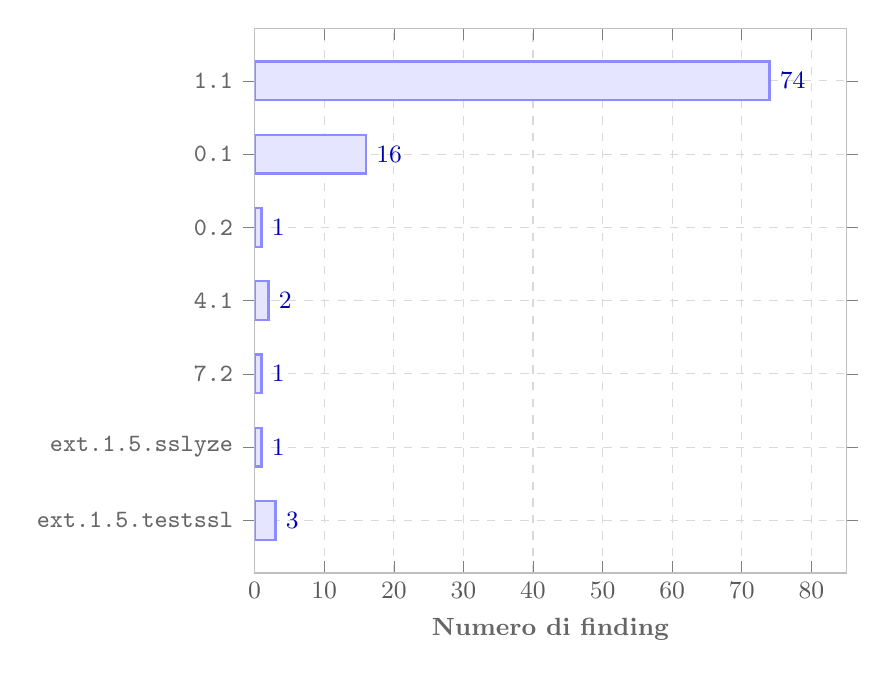
\begin{tikzpicture}
      \begin{axis}[
          xbar,
          width=0.75\textwidth, % <-- CORREZIONE: Lascia il 25% di spazio per le etichette laterali
          height=8.5cm,
          bar width=14pt,
          %
          % Setup Asse X
          xmin=0, xmax=85,
          xtick={0,10,20,30,40,50,60,70,80},
          xlabel={Numero di finding},
          xlabel style={font=\small\bfseries, text=gray!80!black},
          tick label style={font=\small, text=gray!70!black},
          %
          % Setup Asse Y
          symbolic y coords={{ext.1.5.testssl},{ext.1.5.sslyze},{7.2},{4.1},{0.2},{0.1},{1.1}},
          ytick=data,
          yticklabel style={font=\small\ttfamily, text=gray!80!black},
          enlarge y limits=0.12,
          %
          % Griglia
          grid=major,
          grid style={dashed, gray!30},
          axis line style={gray!50},
          %
          % Numeri a fianco delle barre
          nodes near coords,
          nodes near coords align={horizontal},
          every node near coord/.style={font=\small\bfseries, text=blue!70!black},
        ]

        \addplot[fill=blue!10, draw=blue!45, thick] coordinates {
            (3,{ext.1.5.testssl})
            (1,{ext.1.5.sslyze})
            (1,{7.2})
            (2,{4.1})
            (1,{0.2})
            (16,{0.1})
            (74,{1.1})
          };
      \end{axis}
    \end{tikzpicture}
  \end{adjustbox}
  \caption{Distribuzione dei 98 finding per test nell'assessment di validazione.}
  \label{fig:finding-distribution}
\end{figure}

\noindent{\small Cap.~5, §5.3, [DISCUTI] distribuzione 98 finding per test. Verificare ridondanza con tab:risultati-per-test.}
\clearpage

% ── Cap. 6 ───────────────────────────────────────────────────────────────────

% INSERIRE
% Cap. 6, §6.2.1
%
% PRIMA   : "Con codici semanticamente distinti questo routing è automatizzabile senza leggere i log."
% DOPO    : "Sistemi di \gls{CI/CD} come GitHub Actions o GitLab \gls{CI}"
% REF     : modifica frase esistente:
%   PRIMA "Con codici semanticamente distinti questo routing è automatizzabile senza leggere i log."
%   DOPO  "Con codici semanticamente distinti questo routing è automatizzabile senza leggere i log, come schematizzato nella Figura~\ref{fig:cicd-decision-tree}."
\begin{figure}[htbp]
  \centering
  \begin{adjustbox}{max width=\textwidth}
    \begin{tikzpicture}[
        % Stili Gold Standard (niente dipendenze da classi esterne)
        base/.style={draw, rounded corners=1pt, inner sep=6pt, align=center, font=\small, minimum height=3.5ex},
        cmd/.style={base, fill=blue!5, draw=blue!40, font=\small\ttfamily, minimum width=16em},
        decision/.style={draw, shape=diamond, aspect=2.5, inner sep=2pt, align=center, font=\small, fill=orange!10, draw=orange!50},
        %
        % Stili per gli Exit Codes (Larghezza fissa per allineamento a colonna)
        code0/.style={base, fill=green!10, draw=green!50!black, minimum width=8.5em},
        code1/.style={base, fill=red!10, draw=red!60!black, minimum width=8.5em},
        code2/.style={base, fill=orange!10, draw=orange!60!black, minimum width=8.5em},
        code10/.style={base, fill=gray!15, draw=gray!60!black, minimum width=8.5em},
        %
        % Stili per le Actions (Larghezza fissa e generosa)
        act0/.style={base, fill=green!5, draw=green!40, minimum width=13em},
        act1/.style={base, fill=red!5, draw=red!40, minimum width=13em},
        act2/.style={base, fill=orange!5, draw=orange!40, minimum width=13em},
        act10/.style={base, fill=gray!5, draw=gray!40, minimum width=13em},
      ]

      %% ── Asse Centrale (Runner -> Comando -> Decisione) ────────────────────
      \node[base, fill=gray!10, draw=gray!40, font=\small\bfseries] (start) {Runner CI/CD};
      \node[cmd, below=3ex of start] (cmd) {apiguard run -{}-config config.yaml};
      \node[decision, below=3ex of cmd] (dec) {exit code?};

      %% ── Colonna Exit Codes (Ancorati in alto a sx, coordinate forzate) ────
      % Il primo è spostato a destra di 4em rispetto al centro del rombo
      \path (dec.south) ++(4em, -4ex) node[code0, anchor=north west] (e0) {\textbf{\texttt{0}: CLEAN}\\{\scriptsize tutti PASS/SKIP}};
      \path (e0.south west) ++(0, -2.5ex) node[code1, anchor=north west] (e1) {\textbf{\texttt{1}: FAIL}\\{\scriptsize almeno un FAIL}};
      \path (e1.south west) ++(0, -2.5ex) node[code2, anchor=north west] (e2) {\textbf{\texttt{2}: ERROR}\\{\scriptsize ERROR senza FAIL}};
      \path (e2.south west) ++(0, -2.5ex) node[code10, anchor=north west] (e10) {\textbf{\texttt{10}: INFRA}\\{\scriptsize errore infrastrutturale}};

      %% ── Colonna Actions (Ancorate esattamente a 3em a destra dei codici) ──
      \path (e0.east) ++(3em, 0) node[act0, anchor=west] (a0) {\textbf{Pipeline prosegue}\\{\scriptsize (merge / deploy consentito)}};
      \path (e1.east) ++(3em, 0) node[act1, anchor=west] (a1) {\textbf{Blocco merge/deploy}\\{\scriptsize Report allegato come artefatto}};
      \path (e2.east) ++(3em, 0) node[act2, anchor=west] (a2) {\textbf{Alert malfunzionamento}\\{\scriptsize Revisione manuale richiesta}};
      \path (e10.east) ++(3em, 0) node[act10, anchor=west] (a10) {\textbf{Diagnosi deployment}\\{\scriptsize Verifica \texttt{config.yaml}}};

      %% ── Frecce di Flusso Principale ───────────────────────────────────────
      % Uso -latex per garantire la punta della freccia pulita senza dipendere da ag-arr
      \draw[-latex, semithick] (start) -- (cmd);
      \draw[-latex, semithick] (cmd) -- (dec);

      %% ── Routing a Bus per le condizioni (Il tronco verticale) ─────────────
      \coordinate (bus-end) at (dec.south |- e10.west);
      \draw[gray!70, semithick] (dec.south) -- (bus-end);

      % Diramazioni orizzontali verso gli Exit Code (colorate)
      \draw[-latex, semithick, green!50!black] (dec.south |- e0.west) -- (e0.west);
      \fill[gray!70] (dec.south |- e0.west) circle (1.5pt);

      \draw[-latex, semithick, red!60!black] (dec.south |- e1.west) -- (e1.west);
      \fill[gray!70] (dec.south |- e1.west) circle (1.5pt);

      \draw[-latex, semithick, orange!60!black] (dec.south |- e2.west) -- (e2.west);
      \fill[gray!70] (dec.south |- e2.west) circle (1.5pt);

      \draw[-latex, semithick, gray!60!black] (dec.south |- e10.west) -- (e10.west);
      \fill[gray!70] (dec.south |- e10.west) circle (1.5pt);

      %% ── Frecce dalle Condizioni alle Azioni (colorate in scala) ───────────
      \draw[-latex, semithick, green!50!black] (e0.east) -- (a0.west);
      \draw[-latex, semithick, red!60!black] (e1.east) -- (a1.west);
      \draw[-latex, semithick, orange!60!black] (e2.east) -- (a2.west);
      \draw[-latex, semithick, gray!60!black] (e10.east) -- (a10.west);

    \end{tikzpicture}
  \end{adjustbox}
  \caption{Routing degli exit code semantici (D6.P1) nella pipeline \gls{CI/CD}.}
  \label{fig:cicd-decision-tree}
\end{figure}

\noindent{\small Cap.~6, §6.2.1, routing exit code semantici (D6.P1): 0 clean, 1 fail, 2 error, 10 infra.}
\clearpage

% INSERIRE
% Cap. 6, §6.3.2
%
% PRIMA   : "garantendo che i finding prodotti da moduli distinti siano confrontabili nel report finale."
% DOPO    : "\paragraph{Coverage augmentation progressiva.}"
% REF     : aggiungere frase nel corpo del paragrafo prima della figura: La Figura~\ref{fig:modular-platform} illustra l'architettura a stella risultante, con il core invariato e i moduli di protocollo come unità intercambiabili.
\begin{figure}[htbp]
  \centering
  \begin{adjustbox}{max width=\textwidth}
    \begin{tikzpicture}[
        % Distanze calibrate
        node distance=4.5ex and 2.5em,
        %
        % Stili di base
        base/.style={draw, rounded corners=2pt, inner sep=8pt, align=center, font=\small},
        %
        % Core invariante leggermente allargato a 22em per accogliere la nuova riga dei contratti
        core/.style={base, fill=blue!8, draw=blue!45, minimum width=22em, thick},
        % Plugin mantenuto proporzionale (2em in meno del core)
        active/.style={base, fill=green!10, draw=green!50!black, minimum width=20em},
        %
        % Moduli Satelliti
        planned/.style={base, fill=gray!4, draw=gray!40, dashed, minimum width=8em},
        %
        % Stili Frecce
        arr-active/.style={-latex, thick, green!50!black},
        arr-planned/.style={-latex, thick, dashed, gray!50}
      ]

      %% ── Core immutabile (Centro) ──────────────────────────────────────────
      \node[core] (core) {
      \textbf{Core: infrastruttura immutabile}\\[1.5ex]
      {\footnotesize \texttt{Engine} \textbar{} \texttt{DAGScheduler} \textbar{} \texttt{EvidenceStore}}\\[0.8ex]
      {\footnotesize \texttt{TestContext} \textbar{} \texttt{TargetContext}}\\[0.8ex]
      {\footnotesize \texttt{BaseTest} \textbar{} \texttt{BaseConnector} \textbar{} \texttt{BaseGatewayAdapter}}\\[0.8ex]
      {\footnotesize \texttt{TestResult} \textbar{} \texttt{Finding} \textbar{} \texttt{EvidenceRecord}}
      };

      %% ── Moduli Satelliti (A stella) ───────────────────────────────────────
      % Modulo attivo (Sopra)
      \node[active, above=of core] (rest) {
      \textbf{Plugin REST (\gls{OAS})} \ {\footnotesize\itshape (attivo)}\\[1.5ex]
      {\footnotesize \texttt{OpenAPI discovery} \textbar{} \texttt{AttackSurface}}\\[0.8ex]
      {\footnotesize \texttt{SecurityClient} \textbar{} \texttt{KongGatewayAdapter}}\\[0.8ex]
      {\footnotesize 18 Test nativi (Domini D0--D7)}
      };

      % Moduli pianificati (Destra, Sotto, Sinistra)
      \node[planned, right=of core] (gql) {\textbf{GraphQL}\\[0.5ex]{\footnotesize\itshape (pianificato)}};
      \node[planned, below=of core] (grpc) {\textbf{gRPC}\\[0.5ex]{\footnotesize\itshape (pianificato)}};
      \node[planned, left=of core] (ws) {\textbf{WebSocket}\\[0.5ex]{\footnotesize\itshape (pianificato)}};

      %% ── Frecce di Collegamento (Convergenti verso il Core) ────────────────
      \draw[arr-active] (rest.south) -- (core.north);
      \draw[arr-planned] (gql.west) -- (core.east);
      \draw[arr-planned] (grpc.north) -- (core.south);
      \draw[arr-planned] (ws.east) -- (core.west);

      %% ── Legenda e Note ────────────────────────────────────────────────────
      \node[font=\footnotesize, text=gray!80!black, below=4ex of grpc, align=center] (note) {
      frecce continue: modulo attivo \quad frecce tratteggiate: moduli pianificati\\[1ex]
      {\itshape Il discovery dinamico via \texttt{pkgutil} permette il caricamento trasparente di moduli di terze parti}
      };

    \end{tikzpicture}
  \end{adjustbox}
  \caption{Evoluzione di APIGuard Assurance verso una piattaforma modulare: separazione netta tra il core invariante e i plugin di protocollo.}
  \label{fig:modular-platform}
\end{figure}
\noindent{\small Cap.~6, §6.3.2, piattaforma modulare: core immutabile + moduli REST/GraphQL/gRPC/WebSocket.}
\clearpage in main.tex (commentare prima della consegna).

\chapter{Asset test: figure e tabelle}

\makeatletter
\renewcommand{\fps@figure}{H}
\renewcommand{\fps@table}{H}
\makeatother

% ═══════════════════════════════════════════════════════════════════════════════
\section{Tabelle}
% ═══════════════════════════════════════════════════════════════════════════════

% ── Cap. 2 ───────────────────────────────────────────────────────────────────

% INSERIRE
% Cap. 2, §2.2.1
%
% PRIMA   : "Questa caratteristica impone vincoli specifici sulle tipologie di verifica applicabili in sede di assessment."
% DOPO    : "\subsection{Criteri di Selezione e Giustificazione Architetturale} \label{subsec:criteri-selezione}"
% REF     : aggiungere frase nuova prima della tabella: La Tabella~\ref{tab:modelli-esposizione} confronta i quattro modelli lungo le dimensioni rilevanti per il security assessment.
\begin{table}[ht]
  \centering \small
  \begin{tabularx}{\textwidth}{@{} p{3.0cm} p{1.8cm} X X X @{}}
    \toprule
    \textbf{Modello}
     & \textbf{Traffico presidiato}
     & \textbf{Enforcement policy}
     & \textbf{Accesso al piano di configurazione}
     & \textbf{Verifica \texttt{WHITE\_BOX}}           \\
    \midrule
    Gateway \gls{API} Dedicato (es.\ Kong, Apigee)
     & Nord-sud
     & Centralizzato in un unico strato ispezionabile
     & Admin \gls{API} diretta
     & Nativa                                          \\
    \addlinespace
    Kubernetes Ingress / Gateway \gls{API}
     & Nord-sud
     & Parziale: annotation controller-specifiche
     & \texttt{kubectl} / Kubernetes \gls{API}
     & Controller-dipendente                           \\
    \addlinespace
    Service Mesh (es.\ Istio)
     & Est-ovest
     & Distribuito per sidecar proxy
     & Control plane (istiod)
     & Fuori perimetro nord-sud                        \\
    \addlinespace
    Gateway Managed Cloud (AWS, Azure, GCP)
     & Nord-sud
     & Centralizzato: gestito interamente dal provider
     & \gls{SDK} / \gls{API} del cloud provider
     & Richiede adapter dedicato                       \\
    \bottomrule
  \end{tabularx}
  \caption{Confronto dei quattro modelli di esposizione in rete lungo le dimensioni rilevanti per il security assessment: il gateway \gls{API} dedicato è l'unico con Admin \gls{API} diretta e verifica \texttt{WHITE\_BOX} nativa.}
  \label{tab:modelli-esposizione}
\end{table}

\noindent{\small Cap.~2, §2.2.1, confronto modelli di esposizione: enforcement, accesso piano di configurazione, verificabilità WHITE\_BOX.}
\clearpage

% INSERIRE
% Cap. 2, §2.3.1
%
% PRIMA   : "richiesta sintatticamente corretta che viola le assunzioni del sistema sull'identità, i privilegi o il comportamento atteso del chiamante."
% DOPO    : "Colmare il semantic gap richiede che lo strumento disponga di una rappresentazione formale"
% REF     : modifica frase esistente:
%   PRIMA "...sono tutte vulnerabilità semantiche."
%   DOPO  "...sono tutte vulnerabilità semantiche, come sintetizzato nella Tabella~\ref{tab:semantic-gap}."
\begin{table}[ht]
  \centering \small
  \begin{tabularx}{\textwidth}{@{} l l C L @{}}
    \toprule
    \textbf{Vulnerabilità OWASP} & \textbf{Natura} & \textbf{Visibilità WAF/DAST} & \textbf{Prerequisito informativo} \\
    \midrule
    API1:2023: BOLA              & Semantica       & Cieca                        & Token $\geq 2$ ruoli              \\
    \addlinespace
    API2:2023: Broken Auth       & Sin./Sem.       & Parziale                     & Nessuno (BLACK\_BOX)              \\
    \addlinespace
    API3:2023: BOPLA             & Semantica       & Cieca                        & Token autenticato                 \\
    \addlinespace
    API5:2023: BFLA              & Semantica       & Cieca                        & Token $\geq 2$ ruoli              \\
    \addlinespace
    API7:2023: SSRF              & Semantica       & Parziale                     & Nessuno / token                   \\
    \bottomrule
  \end{tabularx}
  \caption{Tassonomia OWASP API Security Top~10 (2023): natura, visibilità WAF/DAST e prerequisito informativo per la rilevazione.}
  \label{tab:semantic-gap}
\end{table}
\noindent{\small Cap.~2, §2.3.1, tassonomia OWASP Top~10 (2023): natura, visibilità WAF/DAST, prerequisito informativo.}
\clearpage

% INSERIRE
% Cap. 2, §2.4.3
%
% PRIMA   : "i verdetti dipendono dalle proprietà definite dall'utente, non da un oracolo derivato dal contratto dell'endpoint."
% DOPO    : (fine del file)
% REF     : aggiungere frase nuova prima della tabella: La Tabella~\ref{tab:testing-comparison} sintetizza le differenze strutturali tra i paradigmi esaminati, riportando per ciascuno il tipo di conoscenza del contratto sfruttata, la disponibilità di un oracle formale e il livello di copertura semantica raggiungibile.
\begin{table}[ht]
  \centering \small
  \begin{tabularx}{\textwidth}{@{} l C C C C @{}}
    \toprule
    \textbf{Paradigma}                & \textbf{Conoscenza contratto} & \textbf{Oracle formale} & \textbf{Riproducibilità} & \textbf{Copertura semantica} \\
    \midrule
    SAST                              & Sorgente                      & Nessuno                 & Alta                     & Bassa                        \\
    \addlinespace
    DAST (ZAP)                        & Nessuna                       & Nessuno                 & Media                    & Bassa                        \\
    \addlinespace
    Fuzzer OAS (RESTler/Schemathesis) & Spec OAS                      & Parziale                & Media                    & Media                        \\
    \addlinespace
    \textbf{APIGuard Assurance}       & \textbf{Spec OAS + config}    & \textbf{OAS formale}    & \textbf{Alta}            & \textbf{Alta}                \\
    \bottomrule
  \end{tabularx}
  \caption{Confronto tra paradigmi di security testing per \gls{API} REST: oracle, riproducibilità e copertura semantica.}
  \label{tab:testing-comparison}
\end{table}

\noindent{\small Cap.~2, §2.4.3, confronto paradigmi: SAST, DAST, Fuzzer OAS, APIGuard (oracle, riproducibilità, copertura semantica).}
\clearpage

% ── Cap. 3 ───────────────────────────────────────────────────────────────────

% FATTO \cmark
% Cap. 3, introduzione capitolo
\begin{table}[ht]
  \centering
  \small
  % Abbandoniamo tabularx. Usiamo l l per il dominio e p{22em} per le proprietà.
  \begin{tabular}{@{} l l >{\raggedright\arraybackslash}p{22em} @{}}
    \toprule
    % Uniamo le prime due colonne solo per l'intestazione
    \multicolumn{2}{@{}l}{\textbf{Dominio}} & \textbf{Proprietà}                                                                                                                                                                                                                                                                                                                             \\
    \midrule
    \textbf{D1}                             & Architettura \& Design          &
    \hyperref[subsec:agnosticismo]{\textbf{D1.P1}}, \hyperref[subsec:dep-flow]{\textbf{D1.P2}}, \hyperref[subsec:split-state]{\textbf{D1.P3}}, \hyperref[subsec:dual-hierarchy]{D1.P4}, \hyperref[subsec:connector-hierarchy]{D1.P5}, \hyperref[subsec:gateway-adapter]{\textbf{D1.P6}}                                                                                                      \\
    \addlinespace
    \textbf{D2}                             & Estensibilità \& Manutenibilità &
    \hyperref[subsec:discovery-impl]{D2.P1}, \hyperref[subsec:dag]{\textbf{D2.P2}}, \hyperref[subsec:connector-hierarchy]{D2.P3}, \hyperref[subsec:connector-injection]{D2.P4}, \hyperref[subsec:auth-layer]{D2.P5}, \hyperref[subsec:connector-classification]{D2.P6}, \hyperref[subsec:path-seed]{D2.P7}, \hyperref[subsec:payload-catalog]{D2.P8}                                         \\
    \addlinespace
    \textbf{D3}                             & Config \& Riproducibilità       &
    \hyperref[subsec:config-driven]{\textbf{D3.P1}}, \hyperref[subsec:openapi-sot]{\textbf{D3.P2}}, \hyperref[subsec:box-gradient]{\textbf{D3.P3}}, \hyperref[subsec:reproducibility]{\textbf{D3.P4}}, \hyperref[subsec:zero-state]{\textbf{D3.P5}}                                                                                                                                          \\
    \addlinespace
    \textbf{D4}                             & Robustezza \& Sicurezza         &
    \hyperref[subsec:evidence-store]{\textbf{D4.P1}}, \hyperref[subsec:sanitization]{D4.P2}, \hyperref[subsec:fail-safe]{D4.P3}, \hyperref[subsec:exception-hierarchy]{D4.P4}, \hyperref[subsec:graceful-degradation]{D4.P5}, \hyperref[subsec:teardown]{D4.P6}, \hyperref[subsec:probing-policy]{D4.P7}, \hyperref[subsec:fail-fast]{D4.P8}, \hyperref[subsec:testresult-invariants]{D4.P9} \\
    \addlinespace
    \textbf{D5}                             & Qualità \& Osservabilità        &
    \hyperref[subsec:traceability]{D5.P1}, \hyperref[subsec:traceability]{D5.P2}, \hyperref[subsec:payload-catalog]{D5.P3}, D5.P4, \hyperref[subsec:dual-audit-trail]{D5.P5}                                                                                                                                                                                                                 \\
    \addlinespace
    \textbf{D6}                             & CI/CD \& DevEx                  &
    \hyperref[subsec:exit-codes]{D6.P1}, D6.P2, \hyperref[subsec:dual-layer-type-safety]{D6.P3}                                                                                                                                                                                                                                                                                              \\
    \addlinespace
    \textbf{D7}                             & Packaging \& Deployment         &
    \hyperref[subsec:connector-hierarchy]{D7.P1}, \hyperref[subsec:agpl-isolation]{D7.P2}, D7.P3                                                                                                                                                                                                                                                                                             \\
    \bottomrule
  \end{tabular}
  \caption{Proprietà APIGuard Assurance per dominio.}
  \label{tab:property-index}
\end{table}
\noindent{\small Cap.~3, intro, mappa delle 39 proprietà architetturali per dominio.}
\clearpage

% FATTO \cmark
% Cap. 3, §3.3.1
\begin{table}[ht]
  \centering
  \small
  % tabularx risolve l'equazione dello spazio: colonna c, colonna l, e il resto a X
  \begin{tabularx}{\textwidth}{@{} c l >{\raggedright\arraybackslash}X @{}}
    \toprule
    \textbf{Dominio} & \textbf{Titolo}                   & \textbf{Ambito di verifica}                                                                                                   \\
    \midrule
    D0               & API Discovery                     & Inventario degli endpoint esposti; rilevazione di Shadow API non documentate nella specifica.                                 \\
    \addlinespace
    D1               & Identity \& Authentication        & Meccanismi di riconoscimento del chiamante; robustezza del trasporto delle credenziali; ciclo di vita e revoca dei \gls{JWT}. \\
    \addlinespace
    D2               & Authorization                     & Logiche di controllo degli accessi; difetti di segregazione orizzontale e verticale (\gls{RBAC}, \gls{BOLA}).                 \\
    \addlinespace
    D3               & Data Integrity                    & Coerenza strutturale dei payload; implementazione delle firme crittografiche (\gls{HMAC}).                                    \\
    \addlinespace
    D4               & Availability \& Resilience        & Difese contro l'esaurimento delle risorse; audit di circuit breaker e soglie di rate limiting.                                \\
    \addlinespace
    D5               & Observability                     & Qualità e tempestività della telemetria generata dal sistema.                                                                 \\
    \addlinespace
    D6               & Configuration \& Hardening        & Rafforzamento della configurazione del gateway; policy di routing; header di sicurezza \gls{HTTP}.                            \\
    \addlinespace
    D7               & Business Logic \& Sensitive Flows & Falle semantiche complesse: elusione dei vincoli di processo, \gls{SSRF}, race condition su operazioni critiche.              \\
    \bottomrule
  \end{tabularx}
  \caption{Domini di Assurance di APIGuard Assurance.}
  \label{tab:domini}
\end{table}
\noindent{\small Cap.~3, §3.3.1, otto domini di assurance con titolo e ambito.}
\clearpage

% DISCUTI
% Cap. 3, §3.3.1
%
% Terza tabella nello stesso contesto di tab:domini e tab:box-gradient. Valutare se integrare le colonne Strategia e Implementato direttamente in tab:domini invece di aggiungere una tabella separata.
%
% PRIMA   : "Questa catena logica si riflette nelle dipendenze dichiarate dai singoli test che operano su questi domini, il cui meccanismo di risoluzione è descritto nella Sezione~\ref{subsec:dag}."
% DOPO    : "Domain-5 occupa una posizione particolare nella tassonomia: il dominio è architetturalmente predisposto"
% REF     : aggiungere frase prima della tabella: La Tabella~\ref{tab:domini-box-gradient} integra la vista precedente con la strategia operativa assegnata a ciascun dominio e lo stato di implementazione nella Milestone~1.
\begin{table}[ht]
  \centering \small
  \begin{tabularx}{\textwidth}{@{} l L C C C @{}}
    \toprule
    \textbf{Dominio}   & \textbf{Oggetto di verifica}          & \textbf{Strategia} & \textbf{Priorità} & \textbf{Implementato}  \\
    \midrule
    D0: Discovery      & Inventario endpoint, Shadow \gls{API} & BLACK/GREY         & P0--P1            & \cmark                 \\
    \addlinespace
    D1: Authentication & Autenticazione, lifecycle token       & BLACK/GREY         & P0--P1            & \cmark                 \\
    \addlinespace
    D2: Authorization  & \gls{RBAC}, \gls{BOLA}, \gls{BFLA}    & GREY               & P1--P2            & \cmark                 \\
    \addlinespace
    D3: Data Integrity & Schema, Mass Assignment               & GREY               & P2                & \cmark                 \\
    \addlinespace
    D4: Availability   & Rate limiting, circuit breaking       & GREY/WHITE         & P1--P2            & \cmark                 \\
    \addlinespace
    D5: Observability  & Log, tracing, audit trail             & WHITE              & P3                & \xmark{} (pianificato) \\
    \addlinespace
    D6: Hardening      & Security headers, config. gateway     & WHITE              & P2--P3            & \cmark                 \\
    \addlinespace
    D7: Business Logic & Flussi sensibili, \gls{SSRF}          & GREY               & P2                & \cmark                 \\
    \bottomrule
  \end{tabularx}
  \caption{Tassonomia degli otto domini di assurance: strategia di testing (Box Gradient D3.P3), priorità e stato implementativo nella versione corrente.}
  \label{tab:domini-box-gradient}
\end{table}

\noindent{\small Cap.~3, §3.3.1, [DISCUTI] domini con strategia Box Gradient e stato implementativo.}
\clearpage

% FATTO \cmark
% Cap. 3, §3.3.2
\begin{table}[ht]
  \centering
  \small
  % L'approccio ibrido perfetto: due colonne naturali e una dinamica a riempimento
  \begin{tabularx}{\textwidth}{@{} l l >{\raggedright\arraybackslash}X @{}}
    \toprule
    \textbf{Strategia}  & \textbf{Prerequisiti}               & \textbf{Razionale}                                                                                                             \\
    \midrule
    \texttt{BLACK\_BOX} & Nessuno (solo accesso di rete)      & Controlli perimetrali applicati dal gateway a qualsiasi interlocutore; simulazione di un attaccante esterno senza credenziali. \\
    \addlinespace
    \texttt{GREY\_BOX}  & Token per $\geq 2$ ruoli distinti   & Garanzie che presuppongono stato autenticato con identità di ruolo distinte; inaccessibili senza credenziali valide.           \\
    \addlinespace
    \texttt{WHITE\_BOX} & Accesso Admin \gls{API} del gateway & Configurazione statica verificabile per ispezione diretta tramite piano di controllo del gateway.                              \\
    \bottomrule
  \end{tabularx}
  \caption{Box Gradient applicato in APIGuard Assurance.}
  \label{tab:box-gradient}
\end{table}
\noindent{\small Cap.~3, §3.3.2, Box Gradient: precondizioni per strategia BLACK/GREY/WHITE.}
\clearpage

% ── Cap. 4 ───────────────────────────────────────────────────────────────────

% FATTO \cmark
% Cap. 4, §4.1
\begin{table}[ht]
  \centering
  \small
  \begin{tabular}{@{}lll@{}}
    \toprule
    \textbf{Fase}                 & \textbf{Cartella}               & \textbf{File}                         \\
    \midrule
    1. Inizializzazione           & \texttt{config/}                & \texttt{loader.py}                    \\
    \addlinespace
    2. OpenAPI Discovery          & \texttt{discovery/}             & \texttt{openapi.py}                   \\
    \addlinespace
    3. Costruzione Contesti       & \texttt{src/}                   & \texttt{engine.py}                    \\
    \addlinespace
    4. Test Discovery e \gls{DAG} & \texttt{tests/}, \texttt{core/} & \texttt{registry.py}, \texttt{dag.py} \\
    \addlinespace
    5. Esecuzione                 & \texttt{src/}                   & \texttt{engine.py}                    \\
    \addlinespace
    6. Teardown                   & \texttt{core/}                  & \texttt{context.py}                   \\
    \addlinespace
    7. Report                     & \texttt{report/}                & \texttt{renderer.py}                  \\
    \bottomrule
  \end{tabular}
  \caption{Fasi della pipeline di assessment (1-2-4 bloccanti; 5-6-7 non-bloccanti).}
  \label{tab:pipeline-fasi}
\end{table}

\noindent{\small Cap.~4, §4.1, fasi della pipeline con mapping cartella/file (1-2-4 bloccanti; 5-6-7 non-bloccanti).}
\clearpage

% FATTO \cmark
% Cap. 4, §4.1.2
%
% Nota: quando si inserisce fig:exception-hierarchy modificare anche la frase
% che introduce questa tabella nel capitolo:
%   PRIMA "...riportate nella Tabella~\ref{tab:exception-hierarchy} con la relativa fase."
%   DOPO  "...riportate nella Tabella~\ref{tab:exception-hierarchy} con la relativa fase, la cui struttura gerarchica è illustrata nella Figura~\ref{fig:exception-hierarchy}."
\begin{table}[ht]
  \centering
  \small
  \begin{tabularx}{\textwidth}{@{}llX@{}}
    \toprule
    \textbf{Classe}                   & \textbf{File}               & \textbf{Comportamento}                                                       \\
    \midrule
    \texttt{ToolBaseError}            & \texttt{exceptions.py}      & Radice della gerarchia; non si solleva direttamente                          \\
    \addlinespace
    \texttt{ConfigurationError}       & \texttt{exceptions.py}      & Fase~1: fatale, config non valida; blocca lo startup                         \\
    \addlinespace
    \texttt{OpenAPILoadError}         & \texttt{exceptions.py}      & Fase~2: fatale, spec irraggiungibile o invalida; blocca lo startup           \\
    \addlinespace
    \texttt{DAGCycleError}            & \texttt{exceptions.py}      & Fase~4: fatale, ciclo nelle dipendenze; blocca lo startup                    \\
    \addlinespace
    \texttt{AuthenticationSetupError} & \texttt{exceptions.py}      & Helper auth: fatale se le credenziali configurate sono invalide              \\
    \addlinespace
    \texttt{SecurityClientError}      & \texttt{exceptions.py}      & Fase~5: recuperata, produce \texttt{TestResult(ERROR)}                       \\
    \addlinespace
    \texttt{ExternalToolError}        & \texttt{exceptions.py}      & Fase~5: recuperata, produce \texttt{TestResult(ERROR)}                       \\
    \addlinespace
    \texttt{TeardownError}            & \texttt{exceptions.py}      & Fase~6: recuperata, registrata come \texttt{WARNING}                         \\
    \addlinespace
    \texttt{GatewayAdapterError}      & \texttt{gateway/base.py}    & Fase~5: recuperata, produce \texttt{TestResult(ERROR)}                       \\
    \addlinespace
    \texttt{SeedGeneratorFetchError}  & \texttt{seed\_generator.py} & \gls{CLI} \texttt{generate-seed}: catturata in \texttt{cli.py}, exit~code~10 \\
    \addlinespace
    \texttt{SeedGeneratorParseError}  & \texttt{seed\_generator.py} & \gls{CLI} \texttt{generate-seed}: catturata in \texttt{cli.py}, exit~code~10 \\
    \bottomrule
  \end{tabularx}
  \caption{Gerarchia delle eccezioni custom (Fasi 1--4 bloccanti; Fasi 5--6 recuperate localmente).}
  \label{tab:exception-hierarchy}
\end{table}

\noindent{\small Cap.~4, §4.1.2 11, eccezioni custom: file e comportamento (bloccanti Fasi~1--4; recuperate Fasi~5--6).}
\clearpage

% ── Cap. 5 ───────────────────────────────────────────────────────────────────

% FATTO \cmark
% Cap. 5, §5.1.1
\begin{table}[ht]
  \centering
  \small
  % Aggiunti i margini invisibili @{} e il raggedright per la colonna X
  \begin{tabularx}{\textwidth}{@{} l l >{\raggedright\arraybackslash}X @{}}
    \toprule
    \textbf{Componente}         & \textbf{Versione}     & \textbf{Ruolo nel testbed}                                                                                  \\
    \midrule
    \texttt{apiguard-assurance} & 0.1.0                 & Tool sotto validazione                                                                                      \\
    \addlinespace
    Python                      & 3.12.3                & Interprete del tool                                                                                         \\
    \addlinespace
    Forgejo                     & 14.0.3 (gitea-1.22.0) & Target applicativo: \gls{API} REST con specifica OpenAPI nativa                                             \\
    \addlinespace
    PostgreSQL                  & 15-alpine             & Backend di persistenza di Forgejo (dipendenza funzionale, non componente autonomo)                          \\
    \addlinespace
    Kong                        & 3.9 DB-less           & \gls{API} Gateway: proxy \gls{HTTP}/\gls{HTTPS}, instradamento verso Forgejo, Admin \gls{API} su porta 8001 \\
    \addlinespace
    \texttt{nuclei}             & 3.8.0                 & Tool esterno per Shadow \gls{API} discovery (test \texttt{ext.0.1})                                         \\
    \addlinespace
    \texttt{nuclei-templates}   & 10.4.3                & Base di template di scansione versioned: garantisce che lo stesso set di firme venga usato in ogni run      \\
    \addlinespace
    \texttt{testssl.sh}         & 3.2.3                 & Analisi \gls{TLS} black-box (test \texttt{ext.1.5.testssl})                                                 \\
    \addlinespace
    \texttt{sslyze}             & (libreria Python)     & Analisi \gls{TLS} via libreria Python (test \texttt{ext.1.5.sslyze})                                        \\
    \bottomrule
  \end{tabularx}
  \caption{Componenti e versioni dell'ambiente di test.}
  \label{tab:versioni-testbed}
\end{table}
\noindent{\small Cap.~5, §5.1.1, componenti e versioni dell'ambiente di test.}
\clearpage

% FATTO \cmark
% Cap. 5, §5.2.1
\begin{table}[ht]
  \centering
  \small
  \begin{tabularx}{\textwidth}{l l X}
    \toprule
    \textbf{Tool}      & \textbf{Esito}               & \textbf{Note}         \\
    \midrule
    \texttt{ruff}      & 0 errori                     &
    Ruleset \texttt{E/W/F/I/N/UP/B/S/ANN}                                     \\
    \addlinespace
    \texttt{mypy}      & 0 errori                     &
    Modalità \texttt{strict}: \texttt{no-implicit-optional},
    \texttt{disallow-untyped-defs}, \texttt{warn-return-any}                  \\
    \addlinespace
    \texttt{bandit}    & 0 finding severity medium$+$ &
    3 Low (B404, S603$\times$2) soppressi con \texttt{\#~noqa} documentati:
    invocazione subprocess controllata per design                             \\
    \addlinespace
    \texttt{vulture}   & 0 finding                    &
    Confidence $\ge$80\%; metodi a dispatching dinamico esclusi via whitelist \\
    \addlinespace
    \texttt{pip-audit} & 0 \gls{CVE}                  &
    Nessuna vulnerabilità nota nelle dipendenze dichiarate                    \\
    \bottomrule
  \end{tabularx}
  \caption{Risultati dell'analisi statica su APIGuard Assurance v0.1.0.}
  \label{tab:analisi-statica}
\end{table}

\noindent{\small Cap.~5, §5.2.1, risultati analisi statica v0.1.0 (ruff, mypy, bandit, vulture, pip-audit).}
\clearpage

% FATTO \cmark
% Cap. 5, §5.2.3
\begin{table}[ht]
  \centering
  \small
  \begin{tabularx}{\textwidth}{l l X}
    \toprule
    \textbf{Aspetto}            & \textbf{Stato} & \textbf{Dettaglio}                                                  \\
    \midrule
    Analisi statica             & \checkmark     &
    0 errori su tutti e cinque gli strumenti (Sezione~\ref{subsec:static-analysis})                                    \\
    \addlinespace
    Type safety                 & \checkmark     &
    0 errori mypy strict; validazione Pydantic attiva su tutti i confini (Sezione~\ref{subsec:dual-layer-type-safety}) \\
    \addlinespace
    Documentazione interna      & \checkmark     &
    292/292 simboli pubblici con docstring (100\%)                                                                     \\
    \addlinespace
    Riproducibilità della build & \checkmark     &
    SHA-256 identico su due build consecutive (451\,261~byte)                                                          \\
    \addlinespace
    Portabilità                 & \checkmark     &
    Cold install in ambiente pulito: \texttt{apiguard version} $\to$ \texttt{0.1.0}                                    \\
    \bottomrule
  \end{tabularx}
  \caption{Sintesi delle verifiche di qualità sulla codebase.}
  \label{tab:verdetto-release}
\end{table}

\noindent{\small Cap.~5, §5.2.3, sintesi verifiche qualità codebase.}
\clearpage

% FATTO \cmark
% Cap. 5, §5.3
\begin{table}[ht]
  \centering
  \small
  \begin{tabularx}{0.85\textwidth}{l C C C}
    \toprule
    \textbf{\gls{KPI}}                     & \textbf{Run~1}    & \textbf{Run~2}    & \textbf{$\Delta$} \\
    \midrule
    PASS / FAIL / SKIP / ERROR             & 9 / 7 / 2 / 0     & 9 / 7 / 2 / 0     & identico          \\
    \addlinespace
    Finding count totale                   & 98                & 98                & identico          \\
    \addlinespace
    \texttt{pass\_rate\_pct}               & 56.2\%            & 56.2\%            & identico          \\
    \addlinespace
    \texttt{assessment\_duration\_seconds} & 290.14\,s         & 290.81\,s         & $+$0.23\%         \\
    \addlinespace
    Exit code / label                      & 1 / \texttt{FAIL} & 1 / \texttt{FAIL} & identico          \\
    \bottomrule
  \end{tabularx}
  \caption{KPI di idempotenza su due run indipendenti.}
  \label{tab:idempotenza-kpi}
\end{table}

\noindent{\small Cap.~5, §5.3, KPI idempotenza su due run indipendenti.}
\clearpage

% FATTO \cmark
% Cap. 5, §5.3
\begin{table}[ht]
  \centering
  \small
  % Tabular puro con margini di 0.5em. Allineamenti: left, left, center, center, center
  \begin{tabular}{@{\hspace{0.5em}} l l c c c @{\hspace{0.5em}}}
    \toprule
    \textbf{Test ID}         & \textbf{Dominio}   & \textbf{Tipo} & \textbf{Status} & \textbf{Finding} \\
    \midrule
    \texttt{0.1}             & D0: Discovery      & Nativo        & \texttt{FAIL}   & 16               \\
    \texttt{0.2}             & D0: Discovery      & Nativo        & \texttt{FAIL}   & 1                \\
    \texttt{0.3}             & D0: Discovery      & Nativo        & \texttt{SKIP}   & 0                \\
    \addlinespace
    \texttt{1.1}             & D1: Auth           & Nativo        & \texttt{FAIL}   & 74               \\
    \texttt{1.4}             & D1: Auth           & Nativo        & \texttt{PASS}   & 0                \\
    \texttt{1.5}             & D1: Auth           & Nativo        & \texttt{PASS}   & 0                \\
    \texttt{1.6}             & D1: Auth           & Nativo        & \texttt{SKIP}   & 0                \\
    \addlinespace
    \texttt{2.1}             & D2: Authorization  & Nativo        & \texttt{PASS}   & 0                \\
    \addlinespace
    \texttt{3.3}             & D3: Data Integrity & Nativo        & \texttt{PASS}   & 0                \\
    \addlinespace
    \texttt{4.1}             & D4: Availability   & Nativo        & \texttt{FAIL}   & 2                \\
    \texttt{4.2}             & D4: Availability   & Nativo        & \texttt{PASS}   & 0                \\
    \texttt{4.3}             & D4: Availability   & Nativo        & \texttt{PASS}   & 0                \\
    \addlinespace
    \texttt{6.2}             & D6: Hardening      & Nativo        & \texttt{PASS}   & 0                \\
    \texttt{6.4}             & D6: Hardening      & Nativo        & \texttt{PASS}   & 0                \\
    \addlinespace
    \texttt{7.2}             & D7: Business Logic & Nativo        & \texttt{FAIL}   & 1                \\
    \addlinespace
    \texttt{ext.0.1.nuclei}  & D0: Discovery      & Esterno       & \texttt{PASS}   & 0                \\
    \texttt{ext.1.5.sslyze}  & D1: Auth           & Esterno       & \texttt{FAIL}   & 1                \\
    \texttt{ext.1.5.testssl} & D1: Auth           & Esterno       & \texttt{FAIL}   & 3                \\
    \midrule
    \textbf{Totale}          &                    &               &                 & \textbf{98}      \\
    \bottomrule
  \end{tabular}
  \caption{Status e finding count per test.}
  \label{tab:risultati-per-test}
\end{table}
\noindent{\small Cap.~5, §5.3, status e finding count per ciascuno dei 18 test.}
\clearpage

% FATTO \cmark
% Cap. 5, §5.4
\begin{table}[ht]
  \centering
  \small
  \begin{tabularx}{\textwidth}{l C C}
    \toprule
    \textbf{Metrica}       & \textbf{Run~1}      & \textbf{Run~2}      \\
    \midrule
    Wall-clock elapsed     & 290.14\,s (4:50.14) & 290.81\,s (4:50.81) \\
    \addlinespace
    User time              & 35.09\,s            & 34.67\,s            \\
    \addlinespace
    System time            & 41.51\,s            & 41.62\,s            \\
    \addlinespace
    Peak resident set size & 287\,MB             & 295\,MB             \\
    \bottomrule
  \end{tabularx}
  \caption{Metriche di sistema sui due run.}
  \label{tab:performance-baseline}
\end{table}

\noindent{\small Cap.~5, §5.4, metriche di sistema sui due run (wall-clock, CPU, memoria).}
\clearpage

% FATTO \cmark
% Cap. 5, §5.4.2
\begin{table}[ht]
  \centering
  \small
  % tabularx per mandare a capo i test.
  % Cardinalità centrata (c) e allineamento a bandiera (raggedright) per evitare spazi dilatati
  \begin{tabularx}{\textwidth}{@{\hspace{0.5em}} l c >{\raggedright\arraybackslash}X @{\hspace{0.5em}}}
    \toprule
    \textbf{Fase DAG}                        & \textbf{Cardinalità} & \textbf{Test}                                                                                                                                                                                                                                                                                           \\
    \midrule
    Phase~A (nessuna dipendenza)             & 16 test              &
    \texttt{0.1} $\cdot$ \texttt{0.2} $\cdot$ \texttt{0.3} $\cdot$ \texttt{1.1} $\cdot$ \texttt{1.5} $\cdot$ \texttt{1.6} $\cdot$ \texttt{3.3} $\cdot$ \texttt{4.1} $\cdot$ \texttt{4.2} $\cdot$ \texttt{4.3} $\cdot$ \texttt{6.2} $\cdot$ \texttt{6.4} $\cdot$ \texttt{7.2} $\cdot$ \texttt{ext.0.1.nuclei} $\cdot$ \texttt{ext.1.5.testssl} $\cdot$ \texttt{ext.1.5.sslyze} \\
    \addlinespace
    Phase~B (\texttt{depends\_on = ["1.1"]}) & 2 test               &
    \texttt{1.4} $\cdot$ \texttt{2.1}                                                                                                                                                                                                                                                                                                                                         \\
    \bottomrule
  \end{tabularx}
  \caption{Topologia del \gls{DAG} nell'assessment di validazione.}
  \label{tab:dag-topology}
\end{table}
\noindent{\small Cap.~5, §5.4.2, topologia DAG: Phase~A (16 test) e Phase~B (\texttt{depends\_on=["1.1"]}).}
\clearpage

% ═══════════════════════════════════════════════════════════════════════════════
\section{Figure}
% ═══════════════════════════════════════════════════════════════════════════════

% ── Cap. 2 ───────────────────────────────────────────────────────────────────

% INSERIRE
% Cap. 2, §2.4.1
%
% PRIMA   : "questo è il limite strutturale del fuzzing cieco applicato alle \gls{API} REST~\cite{MISSING:atlidakis:2019:restler}."
% DOPO    : "Quando invece il contratto è disponibile, la \gls{OAS} diventa la prima e più precisa fonte di conoscenza:"
% REF     : modifica frase esistente:
%   PRIMA "...il limite strutturale del fuzzing cieco applicato alle \gls{API} REST~\cite{MISSING:atlidakis:2019:restler}."
%   DOPO  "...il limite strutturale del fuzzing cieco applicato alle \gls{API} REST~\cite{MISSING:atlidakis:2019:restler}, illustrato schematicamente nella Figura~\ref{fig:combinatorial-wall}."
% ─── FIGURA B (8.1) -- Il Combinatorial Wall ─────────────────────────────────
\begin{figure}[htbp]
  \centering
  \begin{adjustbox}{max width=\textwidth}
    \begin{tikzpicture}[
        % Distanza orizzontale ridotta drasticamente per compattare
        node distance=4ex and 1em,
        %
        % STILE BASE: inner sep ridotto per non sprecare millimetri preziosi
        base/.style={draw, rounded corners=1.5pt, inner sep=3pt, align=center, font=\footnotesize, minimum height=3em},
        %
        % Larghezza colonna 1 ridotta al minimo indispensabile
        col1/.style={minimum width=7.5em},
        %
        % Stili per Via A
        viaA/.style={base, fill=red!6, draw=red!50},
        invis/.style={base, fill=gray!6, draw=gray!40, dashed, text=gray!70!black},
        %
        % Stili per Via B
        viaB/.style={base, fill=green!7, draw=green!45},
        vis/.style={base, fill=green!7, draw=green!50!black},
        %
        lbl/.style={font=\footnotesize\bfseries, inner sep=1pt},
        %
        arrA/.style={-latex, semithick, red!60!black},
        arrB/.style={-latex, semithick, green!50!black},
        arr-wall/.style={-latex, semithick, dashed, gray!60},
        %
        note/.style={font=\scriptsize\itshape, text=gray!70!black, align=center, inner sep=1.5pt}
      ]

      %% ── Via A ─────────────────────────────────────────────────────────────
      \node[viaA, col1] (a1) {Fuzzer\\sintattico};
      % Testo forzato su più righe stringendo il text width
      \node[viaA, right=of a1, text width=6.5em] (a2) {Payload casuali\\malformati};
      \node[viaA, right=of a2, text width=6.5em] (a3) {\texttt{400 Bad}\\\texttt{Request}};

      % Muro combinatorio ridotto a soli 3.5em
      \node[invis, right=3.5em of a3, text width=7em] (a4) {Logica\\applicativa\\{\scriptsize [invisibile]}};

      %% ── Via B ─────────────────────────────────────────────────────────────
      \node[viaB, col1, below=6ex of a1] (b1) {Engine\\contract-driven};

      \node[viaB] (b2) at (a2 |- b1) {Payload validi\\dalla spec \gls{OAS}};
      \node[viaB] (b3) at (a3 |- b1) {\texttt{2xx} / \texttt{4xx}\\semantici};
      \node[vis]  (b4) at (a4 |- b1) {Logica\\applicativa\\{\scriptsize [visibile]}};

      %% ── Etichette di corsia ────────────────────────────────────────────────
      % Distanza minima per recuperare spazio sul margine sinistro estremo
      \node[lbl, text=red!70!black, left=1em of a1] (lblA) {Via~A};
      \node[lbl, text=green!60!black] (lblB) at (lblA |- b1) {Via~B};

      %% ── Frecce Via A ───────────────────────────────────────────────────────
      \draw[arrA] (a1) -- (a2);
      \draw[arrA] (a2) -- (a3);
      % Scritta spostata SOTTO e abbassata leggermente con yshift
      \draw[arr-wall] (a3) -- node[midway, below, yshift=-0.5ex, note] {muro\\combinatorio} (a4);

      %% ── Frecce Via B ───────────────────────────────────────────────────────
      \draw[arrB] (b1) -- (b2);
      \draw[arrB] (b2) -- (b3);
      \draw[arrB] (b3) -- (b4);

      %% ── Linea di Separazione ───────────────────────────────────────────────
      \path (a1.south) ++(0, -3ex) coordinate (mid-y);
      \draw[gray!40, dashed, thick] ([xshift=-0.5em]lblA.west |- mid-y) -- ([xshift=0.5em]a4.east |- mid-y);

    \end{tikzpicture}%
  \end{adjustbox}
  \caption{Il \emph{combinatorial wall}: fuzzer sintattico (Via~A) vs.\ approccio contract-driven \gls{OAS} (Via~B).}
  \label{fig:combinatorial-wall}
\end{figure}
\noindent{\small Cap.~2, §2.4.1, combinatorial wall: fuzzer sintattico (Via~A) vs.\ engine contract-driven OAS (Via~B).}
\clearpage

% ── Cap. 3 ───────────────────────────────────────────────────────────────────

% INSERIRE
% Cap. 3, §3.2
%
% PRIMA   : "Le proprietà discusse nella sezione precedente costituiscono la base del sistema. Le scelte di questa sezione si aggiungono ad esse, ciascuna rispondendo a un'esigenza architetturale specifica che le proprietà fondamentali lasciano aperta."
% DOPO    : "\subsection{Flusso di Dipendenze Monodirezionale (D1.P2)} \label{subsec:dep-flow}"
% REF     : modifica prima frase di sec:architettura:
%   PRIMA "Le proprietà discusse nella sezione precedente costituiscono la base del sistema."
%   DOPO  "Le proprietà discusse nella sezione precedente costituiscono la base del sistema, i cui componenti principali e le loro relazioni sono illustrati nella Figura~\ref{fig:architettura-apiguard}."
\begin{figure}[ht]
  \centering
  % NIENTE \resizebox: il diagramma è ottimizzato per rientrare nella pagina
  % garantendo che i font \footnotesize vengano stampati alla loro vera grandezza.
  \begin{tikzpicture}[
      node distance=1.5ex and 2.5em,
      %
      % Stili di base Gold Standard
      base/.style={draw, rounded corners=1.5pt, inner sep=5pt, align=center, font=\small},
      %
      % Colonne snellite e uniformate (minimum height=3em per i blocchi principali)
      col-in/.style={base, fill=gray!10, draw=gray!50, minimum width=10em},
      col-mid-blue/.style={base, fill=blue!7, draw=blue!40, minimum width=14em, minimum height=3em},
      col-mid-green/.style={base, fill=green!7, draw=green!45, minimum width=14em, minimum height=3em},
      col-mid-gold/.style={base, fill=orange!10, draw=orange!50, minimum width=14em, minimum height=2.5em},
      col-mid-violet/.style={base, fill=violet!7, draw=violet!40, minimum width=14em, minimum height=3em},
      col-out/.style={base, fill=gray!8, draw=gray!50, minimum width=9.5em},
      %
      % Frecce ortogonali pulite
      arr/.style={-latex, semithick, gray!80!black},
      darr/.style={-latex, semithick, dashed, gray!80!black},
      barr/.style={latex-latex, semithick, gray!80!black},
      %
      % Etichette sulle frecce
      lbl/.style={font=\footnotesize\itshape, text=gray!70!black, inner sep=3pt},
      %
      % Sfondo per raggruppamento dinamico
      bg-engine/.style={draw=blue!30, fill=blue!3, dashed, rounded corners=3pt, inner sep=10pt}
    ]

    %% ── Engine (Colonna Centrale) Fissato per primo ──────────────────────
    % Altezza normalizzata tramite lo stile col-mid-blue
    \node[col-mid-blue] (tc) {\textbf{\texttt{TargetContext}} {\footnotesize[frozen]}\\{\footnotesize base\_url | attack\_surface | creds}};

    \node[col-mid-green, below=of tc] (tx) {\textbf{\texttt{TestContext}} {\footnotesize[mutable]}\\{\footnotesize token | teardown | shared\_data}};
    \node[col-mid-gold, below=of tx] (dag) {\textbf{DAG Scheduler}\\{\footnotesize ordinamento, batch sequenziali}};

    %% Box di raggruppamento dinamico (Assessment Engine)
    \begin{scope}[on background layer]
      \node[bg-engine, fit=(tc)(tx)(dag)] (engine) {};
    \end{scope}

    % Etichetta agganciata in alto a sinistra
    \node[font=\footnotesize\bfseries, text=blue!70!black, anchor=south east, shift={(-1em, 0.5ex)}]
    at (engine.north) {Assessment Engine};

    %% ── Input (Colonna Sinistra) Ancorati matematicamente ────────────────
    % Config.yaml: Allineato esattamente col tetto dell'engine (che ora si è abbassato proporzionalmente)
    \node[col-in, anchor=north east] (cfg) at ([xshift=-2.5em]tc.west |- engine.north) {\textbf{\texttt{config.yaml}}\\{\footnotesize credenziali, URL, param.}};

    % OpenAPI.yaml: Più in basso
    \node[col-in, anchor=east] (oas) at ([xshift=-2.5em, yshift=-7ex]tc.west) {\textbf{\texttt{openapi.yaml}}\\{\footnotesize spec formale target}};

    %% ── Target (Colonna Destra) ────────────────────────────────────────────
    \node[col-out, right=6em of tc] (kong) {\textbf{Kong Gateway}\\{\footnotesize :8000 / :8443 / :8001}};

    % Forgejo abbassato ulteriormente (8.5ex) per fare molto spazio all'etichetta Admin API
    \node[col-out, below=8.5ex of kong] (forgejo) {\textbf{Forgejo}\\{\footnotesize target applicativo}};

    %% ── EvidenceStore (Sotto l'Engine) ─────────────────────────────────────
    \node[col-mid-violet, below=4ex of dag] (ev) {\textbf{EvidenceStore} {\footnotesize[JSONL]}\\{\footnotesize \texttt{evidence.json} | \texttt{report.html}}};

    %% ── FRECCE E COLLEGAMENTI ──────────────────────────────────────────────

    %% Input -> Engine
    % config.yaml: Nessuna curva. Va dritto al TargetContext.
    \draw[arr] (cfg.east) -- (tc.west |- cfg.east);

    % openapi.yaml: Esce dall'alto, sale e curva entrando nella metà inferiore del TargetContext (-2ex)
    \draw[arr] (oas.north) |- ([yshift=-2ex]tc.west);

    %% Engine -> Target (Probe HTTP su due righe)
    \path (tc.east) ++(0, 1.5ex) coordinate (probe-start);
    \path (kong.west) ++(0, 1.5ex) coordinate (probe-end);
    \draw[arr] (probe-start) -- node[midway, above, align=center, lbl] {probe\\\gls{HTTP}} (probe-end);

    \draw[barr] (kong.south) -- (forgejo.north);

    %% Interne Engine -> Evidence
    \draw[arr] (dag.north) -- (tx.south);
    \draw[arr] (dag.south) -- (ev.north);

    %% Engine -> Target (Admin API - WHITE_BOX)
    \path (tx.east) ++(0, -1ex) coordinate (admin-start);
    \path (kong.west) ++(0, -1.5ex) coordinate (admin-end);

    % Punto di svolta inferiore (a 2.5em da TestContext)
    \path (admin-start) ++(2.5em, 0) coordinate (admin-turn1);

    % Punto di svolta superiore (l'angolo a 90° prima di entrare in Kong)
    \coordinate (admin-turn2) at (admin-turn1 |- admin-end);

    % Freccia strutturale pulita
    \draw[darr] (admin-start) -- (admin-turn1) -- (admin-turn2) -- (admin-end);

    % Etichetta posizionata incastonata nello spazio vuoto.
    % Spostata più in basso (yshift=-2ex) e leggermente più a sinistra (xshift=0.2em)
    \node[lbl, align=left, anchor=north west]
    at ([xshift=0.2em, yshift=-2ex]admin-turn2)
    {Admin \gls{API}\\{\footnotesize WHITE\_BOX}};

  \end{tikzpicture}
  \caption{Architettura di APIGuard Assurance: Engine, DAG Scheduler ed EvidenceStore.}
  \label{fig:architettura-apiguard}
\end{figure}

\noindent{\small Cap.~3, §3.2, architettura alto livello: input, Engine (Split State D1.P3), DAG Scheduler (D2.P2), EvidenceStore (D4.P1).}
\clearpage

% INSERIRE
% Cap. 3, §3.2.2
%
% PRIMA   : "Salvaguardia contro lo stallo: se il grafo risulta ancora attivo ma non riesce a estrarre nessun test pronto, il sistema emette un errore strutturato che elenca i test mai schedulati e interrompe l'esecuzione in modo controllato, fornendo all'operatore la diagnostica necessaria senza dover ricostruire lo stato interno del grafo."
% DOPO    : "L'ordinamento topologico puro non garantisce un ordine unico tra test pronti allo stesso livello:"
% REF     : aggiungere frase nuova dopo la chiusura del blocco itemize: La topologia del \gls{DAG} nell'assessment di validazione, con le due fasi di esecuzione risultanti, è illustrata nella Figura~\ref{fig:dag-topology}.
\begin{figure}[ht]
  \centering
  % NIENTE \resizebox: il diagramma usa font \footnotesize integrati e spazi 
  % calibrati per rientrare perfettamente nei margini mantenendo i testi nitidi.
  \begin{tikzpicture}[
      node distance=1.5ex and 1em,
      %
      % Stili dei Nodi (indipendenti dal preambolo)
      tst/.style={draw=orange!55, fill=yellow!18, rounded corners=1.5pt, minimum width=4.5em, minimum height=3.5ex, font=\footnotesize\ttfamily, align=center},
      tst-hl/.style={tst, draw=orange!70, fill=yellow!35, thick},
      ext/.style={tst, minimum width=6.5em, font=\scriptsize\ttfamily},
      %
      phB/.style={draw=blue!40, fill=blue!7, rounded corners=1.5pt, minimum width=5.5em, minimum height=3.5ex, font=\footnotesize\ttfamily, align=center},
      phC/.style={draw=gray!40, fill=gray!8, dashed, rounded corners=1.5pt, minimum width=7em, minimum height=4.5ex, font=\footnotesize, align=center},
      %
      % Stili dei Riquadri di Sfondo
      bg-A/.style={draw=orange!50, fill=yellow!6, dashed, rounded corners=3pt, inner sep=12pt},
      bg-B/.style={draw=blue!40, fill=blue!4, dashed, rounded corners=3pt, inner sep=10pt},
      %
      % Frecce native
      arr/.style={-latex, semithick, blue!60},
      darr/.style={-latex, semithick, dashed, gray!60}
    ]

    %% ── Phase A: 16 test (Griglia compatta) ───────────────────────────────
    % D0
    \node[tst] (d0a) {0.1};
    \node[tst, right=of d0a] (d0b) {0.2};
    \node[tst, right=of d0b] (d0c) {0.3};

    % D1 (ORDINE CORRETTO: 1.1 evidenziato a sinistra)
    \node[tst-hl, below=of d0a] (a11) {\textbf{1.1}};
    \node[tst, right=of a11] (d1b) {1.5};
    \node[tst, right=of d1b] (d1c) {1.6};

    % D3 (Gap maggiorato a 3.5ex per creare un "tunnel" orizzontale)
    \node[tst, below=3.5ex of a11] (d3a) {3.3};

    % D4
    \node[tst, below=of d3a] (d4a) {4.1};
    \node[tst, right=of d4a] (d4b) {4.2};
    \node[tst, right=of d4b] (d4c) {4.3};

    % D6
    \node[tst, below=of d4a] (d6a) {6.2};
    \node[tst, right=of d6a] (d6b) {6.4};

    % D7
    \node[tst, below=of d6a] (d7a) {7.2};

    % External tests: MANDATI A CAPO per contenere la larghezza totale di Phase A
    \node[ext, below=of d7a.south west, anchor=north west] (ex0) {ext.0.1.nuclei};
    \node[ext, below=of ex0.south west, anchor=north west] (ex1) {ext.1.5.sslyze};
    \node[ext, right=of ex1] (ex2) {ext.1.5.testssl};

    %% Box Phase A (Includiamo d1c per garantire che abbracci l'estrema destra)
    \begin{scope}[on background layer]
      \node[bg-A, fit=(d0a)(d0c)(a11)(d1c)(d7a)(ex1)(ex2)] (phaseA) {};
    \end{scope}

    % Etichetta Phase A ancorata sopra senza toccare il tratteggio
    \node[font=\footnotesize\bfseries, text=orange!80!black, anchor=south west]
    at ([xshift=1ex, yshift=0.5ex]phaseA.north west) {Phase A (16 test, nessuna dipendenza)};

    %% ── Snodo e Phase B (Biforcazione Simmetrica Esterna) ─────────────────
    % 1. Calcolo del tunnel: scendiamo a metà esatta del gap (1.75ex sotto a 1.1)
    \path (a11.south) ++(0, -1.75ex) coordinate (bus-y);

    % 2. Punto di uscita dal box giallo
    \path (phaseA.east |- bus-y) coordinate (exitA);

    % 3. Snodo matematico: 3.5em di distanza a destra del box giallo
    \path (exitA) ++(3.5em, 0) coordinate (split);

    % I due test di Phase B allineati verticalmente allo snodo
    \node[phB] (b14) at ([xshift=5.5em, yshift=3ex]split) {1.4};
    \node[phB] (b21) at ([xshift=5.5em, yshift=-3ex]split) {2.1};

    %% Box Phase B
    \begin{scope}[on background layer]
      \node[bg-B, fit=(b14)(b21)] (phaseB) {};
    \end{scope}

    % Etichetta Phase B ancorata pulita
    \node[font=\footnotesize\bfseries, text=blue!80!black, anchor=south west]
    at ([xshift=1ex, yshift=0.5ex]phaseB.north west) {Phase B (\texttt{depends\_on=["1.1"]})};

    %% ── Phase C: pianificata ──────────────────────────────────────────────
    % Allineata esattamente all'asse centrale del blocco Phase B
    \node[phC, right=1em of phaseB] (phaseC) at ([xshift=5em]phaseB.east |- split) {\textit{Phase C}\\{\scriptsize (pianificata)}};

    %% ── Frecce di Collegamento e Routing ──────────────────────────────────

    % Il tronco principale: da 1.1.south fa un angolo retto verso il tunnel (|-), 
    % attraversa tutto il box giallo fino all'uscita, e continua fino allo snodo.
    \draw[blue!60, semithick] (a11.south) |- (exitA) --
    node[above, font=\scriptsize\itshape, text=gray!80!black] {\texttt{1.1} $\rightarrow$} (split);

    % Biforcazioni dallo snodo verso i test in Phase B
    \draw[arr] (split) |- (b14.west);
    \draw[arr] (split) |- (b21.west);

    % Freccia verso Phase C (con etichetta generica)
    \draw[darr] (phaseB.east |- split) -- node[above, font=\scriptsize\itshape, text=gray!80!black] {dipendenze} (phaseC.west |- split);

  \end{tikzpicture}
  \caption{Topologia del \gls{DAG} nel ciclo di assessment corrente: Phase~A (nessuna dipendenza), Phase~B (\texttt{depends\_on=["1.1"]}) e Phase~C (pianificata).}
  \label{fig:dag-topology}
\end{figure}

\noindent{\small Cap.~3, §3.2.2, topologia DAG: Phase~A (16 test), Phase~B (\texttt{depends\_on=["1.1"]}), Phase~C pianificata.}
\clearpage

% ── Cap. 4 ───────────────────────────────────────────────────────────────────

% INSERIRE
% Cap. 4, §4.1
%
% PRIMA   : "nessuno di questi moduli importa da \texttt{engine.py}."
% DOPO    : "\subsection{Fail-Safe Error Isolation (D4.P3)} \label{subsec:fail-safe}"
% REF     : aggiungere frase alla fine del paragrafo su engine.py:
%   PRIMA "...nessuno di questi moduli importa da \texttt{engine.py}."
%   DOPO  "...nessuno di questi moduli importa da \texttt{engine.py}. Il flusso completo della pipeline con le condizioni di errore per ciascuna fase è sintetizzato nella Figura~\ref{fig:pipeline-flowchart}."
\begin{figure}[ht]
  \centering
  % NIENTE \resizebox: ottimizzato orizzontalmente per far rientrare la grafica 
  % nei margini e lasciare che i font \footnotesize si renderizzino alla loro grandezza reale.
  \begin{tikzpicture}[
      % Distanza orizzontale compatta per accorciare le frecce laterali
      node distance=3.5ex and 4.5em,
      %
      % Stili di base
      base/.style={draw, rounded corners=1.5pt, inner sep=5pt, align=center, font=\small, minimum height=4.5ex},
      %
      % Stili Fasi (Colonna Sinistra)
      phase-startup/.style={base, fill=blue!7, draw=blue!40, minimum width=13.5em},
      phase-exec/.style={base, fill=green!7, draw=green!45, minimum width=13.5em},
      %
      % Stili Errori (Colonna Destra)
      err-stop/.style={base, fill=red!6, draw=red!50, minimum width=12.5em},
      err-warn/.style={base, fill=orange!8, draw=orange!50, minimum width=12.5em},
      %
      % Terminali (Inizio/Fine)
      term/.style={draw=gray!50, fill=gray!15, ellipse, minimum height=3.5ex, inner sep=5pt, align=center, font=\footnotesize\ttfamily},
      %
      % Testi secondari sulle frecce (inner sep=3pt aggiunto per distaccarle dai fili)
      lbl/.style={font=\footnotesize\itshape, text=gray!70!black, inner sep=3pt},
      %
      % Frecce ortogonali
      arr-ok/.style={-latex, semithick, gray!70!black},
      arr-ko/.style={-latex, semithick, red!60!black},
      arr-warn/.style={-latex, semithick, dashed, orange!80!black},
      %
      % Sfondi per raggruppamento dinamico (Libreria fit)
      bg-startup/.style={draw=blue!30, fill=blue!3, dashed, rounded corners=3pt, inner sep=10pt},
      bg-exec/.style={draw=green!35, fill=green!2, dashed, rounded corners=3pt, inner sep=10pt}
    ]

    %% ── Terminale di avvio ─────────────────────────────────────────────────
    \node[term] (start) {apiguard run};

    %% ── Fasi 1-4 (zona startup, bloccanti) ─────────────────────────────────
    % Spazio a 8ex per creare il corridoio d'ingresso
    \node[phase-startup, below=8ex of start] (p1) {\textbf{Fase~1:} Inizializzazione\\{\footnotesize\texttt{config/loader.py}}};
    \node[phase-startup, below=of p1]    (p2) {\textbf{Fase~2:} OpenAPI Discovery\\{\footnotesize\texttt{discovery/openapi.py}}};
    \node[phase-startup, below=of p2]    (p3) {\textbf{Fase~3:} Costruzione Contesti\\{\footnotesize\texttt{engine.py}}};
    \node[phase-startup, below=of p3]    (p4) {\textbf{Fase~4:} Test Discovery e \gls{DAG}\\{\footnotesize\texttt{registry.py, dag.py}}};

    %% ── Fasi 5-7 (zona esecuzione, non bloccanti) ──────────────────────────
    % GAP ridotto: spazio a 9ex (lascia 5ex netti tra i due box di background)
    \node[phase-exec, below=9ex of p4] (p5) {\textbf{Fase~5:} Esecuzione (per test)\\{\footnotesize\texttt{engine.py}}};
    \node[phase-exec, below=of p5]   (p6) {\textbf{Fase~6:} Teardown \gls{LIFO}\\{\footnotesize\texttt{core/context.py}}};
    \node[phase-exec, below=of p6]   (p7) {\textbf{Fase~7:} Report\\{\footnotesize\texttt{report/renderer.py}}};

    %% ── Terminale di uscita ────────────────────────────────────────────────
    \node[term, below=5ex of p7] (end) {exit code: 0 / 1 / 2 / 10};

    %% ── Rami KO → STOP (fasi bloccanti) posizionati prima degli sfondi ─────
    \node[err-stop, right=4.5em of p1] (s1) {\texttt{ConfigurationError}\\{\footnotesize avvio interrotto}};
    \node[err-stop, right=4.5em of p2] (s2) {\texttt{OpenAPILoadError}\\{\footnotesize avvio interrotto}};
    \node[err-stop, right=4.5em of p4] (s4) {\texttt{DAGCycleError}\\{\footnotesize avvio interrotto}};

    %% ── Rami errore recuperabile (fasi 5, 6) ───────────────────────────────
    \node[err-warn, right=4.5em of p5] (w5) {\texttt{TestResult(ERROR)}\\{\footnotesize isolato, pipeline prosegue}};
    \node[err-warn, right=4.5em of p6] (w6) {\texttt{TeardownError}\\{\footnotesize \texttt{WARNING} strutturato}};

    %% ── Sfondi per le due zone ─────────────────────────────────────────────
    \begin{scope}[on background layer]
      \node[bg-startup, fit=(p1)(p2)(p3)(p4)] (grp-startup) {};
      \node[bg-exec, fit=(p5)(p6)(p7)] (grp-exec) {};
    \end{scope}

    %% ── ETICHETTE DI GRUPPO (Avvicinate all'asse e centrate in Y) ──────────
    % xshift=-0.6em le avvicina notevolmente alla freccia centrale
    % yshift=3ex solleva la prima etichetta al centro matematico del gap superiore.
    \node[font=\footnotesize\bfseries, text=blue!70!black, anchor=east]
    at ([xshift=-0.6em, yshift=3ex]grp-startup.north) {Fasi 1-4 (bloccanti)};

    % yshift=2.5ex solleva la seconda etichetta al centro matematico del gap centrale di 5ex netti.
    \node[font=\footnotesize\bfseries, text=green!70!black, anchor=east]
    at ([xshift=-0.6em, yshift=2.5ex]grp-exec.north) {Fasi 5-7 (non bloccanti)};

    %% ── Frecce asse principale ─────────────────────────────────────────────
    \draw[arr-ok] (start) -- (p1);
    \draw[arr-ok] (p1) -- node[midway, right, lbl] {OK} (p2);
    \draw[arr-ok] (p2) -- node[midway, right, lbl] {OK} (p3);
    \draw[arr-ok] (p3) -- node[midway, right, lbl] {OK} (p4);
    \draw[arr-ok] (p4) -- node[midway, right, lbl] {OK} (p5);
    \draw[arr-ok] (p5) -- (p6);
    \draw[arr-ok] (p6) -- node[midway, right, lbl] {OK} (p7);
    \draw[arr-ok] (p7) -- (end);

    %% ── Frecce Laterali (Centrate nello spazio vuoto ricalibrato a pos=0.55) 
    % Il valore 0.55 arretra i testi rispetto al 0.65 precedente, staccandoli dai riquadri di destra
    \draw[arr-ko] (p1.east) -- node[pos=0.55, above, lbl, text=red!70!black] {KO} (s1.west);
    \draw[arr-ko] (p2.east) -- node[pos=0.55, above, lbl, text=red!70!black] {KO} (s2.west);
    \draw[arr-ko] (p4.east) -- node[pos=0.55, above, lbl, text=red!70!black] {KO} (s4.west);

    \draw[arr-warn] (p5.east) -- node[pos=0.55, above, align=center, lbl, text=orange!80!black] {eccezione\\interna} (w5.west);
    \draw[arr-warn] (p6.east) -- node[pos=0.55, above, align=center, lbl, text=orange!80!black] {cleanup\\parziale} (w6.west);

  \end{tikzpicture}
  \caption{Flusso della pipeline a sette fasi (D4.P3, D4.P4): la zona di startup (Fasi~1-4) è bloccante, un errore in una qualsiasi di esse interrompe l'avvio; la zona di esecuzione (Fasi~5-7) è non bloccante, ogni malfunzionamento è recuperato localmente senza invalidare i risultati già prodotti. Frecce continue: percorso nominale; frecce tratteggiate: errori recuperati con \texttt{WARNING}.}
  \label{fig:pipeline-flowchart}
\end{figure}
\noindent{\small Cap.~4, §4.1, pipeline a 7 fasi: zona startup bloccante (Fasi~1--4) e zona esecuzione non bloccante (Fasi~5--7).}
\clearpage

% FATTO \cmark
% Cap. 4, §4.1
\begin{figure}[ht]
  \dirtree{%
    .1 src/.
    .2 cli.py \normalfont\textit{(entry point \gls{CLI})}.
    .2 engine.py \normalfont\textit{(orchestratore, Fasi 3 e 5)}.
    .2 config/ \normalfont\textit{(Fase 1)}.
    .3 loader.py.
    .2 discovery/ \normalfont\textit{(Fase 2)}.
    .3 openapi.py.
    .3 surface.py.
    .2 core/ \normalfont\textit{(layer fondamentale, Fasi 3--5)}.
    .3 context.py \normalfont\textit{(Fase 3)}.
    .3 evidence.py \normalfont\textit{(Fase 3)}.
    .3 dag.py \normalfont\textit{(Fase 4)}.
    .3 client.py \normalfont\textit{(Fase 5)}.
    .3 exceptions.py.
    .3 gateway/.
    .2 tests/ \normalfont\textit{(Fasi 4--5)}.
    .3 registry.py \normalfont\textit{(Fase 4)}.
    .3 base.py.
    .3 helpers/.
    .3 domain\_0/ \normalfont\textit{... domain\_7/}.
    .2 external\_tests/ \normalfont\textit{(Fasi 4--5)}.
    .3 registry.py \normalfont\textit{(Fase 4)}.
    .3 base.py.
    .2 connectors/ \normalfont\textit{(Fase 5)}.
    .2 report/ \normalfont\textit{(Fase 7)}.
    .3 builder.py.
    .3 renderer.py.
    .3 templates/.
  }
  \caption{Layout di \texttt{src/} con mapping alle fasi della pipeline.}
  \label{fig:src-layout}
\end{figure}

\noindent{\small Cap.~4, §4.1, layout \texttt{src/} con mapping di ogni modulo alla fase della pipeline.}
\clearpage

% INSERIRE
% Cap. 4, §4.1.1
%
% PRIMA   : "La solidità complessiva del sistema non è condizionata dalla correttezza di nessun singolo test."
% DOPO    : "\subsection{Gerarchia delle Eccezioni con Phase Mapping (D4.P4)} \label{subsec:exception-hierarchy}"
% REF     : modifica ultima frase di subsec:fail-safe:
%   PRIMA "La solidità complessiva del sistema non è condizionata dalla correttezza di nessun singolo test."
%   DOPO  "La solidità complessiva del sistema non è condizionata dalla correttezza di nessun singolo test, come illustrato dal sequence diagram in Figura~\ref{fig:sequence-error-isolation}."
\begin{figure}[htbp]
  \centering
  \begin{adjustbox}{max width=\textwidth}
    \begin{tikzpicture}[
        % Attori a 7em e corridoi allargati a 3.2em per riempire la larghezza della pagina
        actor/.style={ag-blue, minimum width=7em, minimum height=2.5em, align=center, font=\small},
        lifeline/.style={draw=gray!50, dashed, very thin},
        msg/.style={ag-arr, black!70},
        msg-return/.style={ag-darr, black!50},
        % Stile unificato per le scritte sulle frecce (con sfondo bianco anti-collisione)
        lbl/.style={midway, above, font=\footnotesize, fill=white, inner sep=2pt},
        % Box per le note
        note-box/.style={draw=orange!50, fill=yellow!12, rounded corners=2pt, inner sep=3pt, font=\footnotesize},
      ]

      %% Attori
      \node[actor] (Eng) {\texttt{Engine}};
      \node[actor, right=3.2em of Eng] (BT) {\texttt{BaseTest}};
      \node[actor, right=3.2em of BT] (SC) {\texttt{SecurityClient}};
      \node[actor, right=3.2em of SC] (TGT) {Target (Kong)};

      %% Lifelines (Allungate a -55ex)
      \draw[lifeline] (Eng.south) -- ++(0,-55ex);
      \draw[lifeline] (BT.south) -- ++(0,-55ex);
      \draw[lifeline] (SC.south) -- ++(0,-55ex);
      \draw[lifeline] (TGT.south) -- ++(0,-55ex);

      %% Scenario normale
      \draw[msg] ([yshift=-4ex]Eng.south) -- ([yshift=-4ex]BT.south) node[lbl] {\texttt{execute(target, ctx)}};
      \draw[msg] ([yshift=-8ex]BT.south) -- ([yshift=-8ex]SC.south) node[lbl] {\texttt{request(method, url, ...)}};
      \draw[msg] ([yshift=-12ex]SC.south) -- ([yshift=-12ex]TGT.south) node[lbl] {\gls{HTTP} request};
      \draw[msg-return] ([yshift=-16ex]TGT.south) -- ([yshift=-16ex]SC.south) node[lbl] {\gls{HTTP} response};
      \draw[msg-return] ([yshift=-20ex]SC.south) -- ([yshift=-20ex]BT.south) node[lbl] {\texttt{Response}};
      \draw[msg-return] ([yshift=-24ex]BT.south) -- ([yshift=-24ex]Eng.south) node[lbl] {\texttt{TestResult(PASS | FAIL)}};

      %% Separatore scenari
      \draw[gray!60, very thick] ([yshift=-28ex]Eng.south) -- ([yshift=-28ex]TGT.south);
      \node[fill=gray!15, draw=gray!60, rounded corners=2pt, inner sep=3pt, font=\footnotesize\itshape]
      at ($([yshift=-28ex]Eng.south)!0.5!([yshift=-28ex]TGT.south)$)
      {scenario alternativo: eccezione imprevista};

      %% Scenario eccezione
      \draw[msg] ([yshift=-34ex]Eng.south) -- ([yshift=-34ex]BT.south) node[lbl] {\texttt{execute(target, ctx)}};
      \draw[msg] ([yshift=-38ex]BT.south) -- ([yshift=-38ex]SC.south) node[lbl] {\texttt{request(method, url, ...)}};

      %% Punto di partenza eccezione
      \coordinate (err_start) at ([yshift=-42ex]SC.south);

      %% Box eccezione
      \node[note-box] (exc) at ($([yshift=-42ex]SC.south)!0.7!([yshift=-42ex]TGT.south)$) {\texttt{Exception} imprevista};

      \draw[ag-arr, orange!70] (err_start) -- (exc.west);

      %% Label catturata internamente
      \coordinate (bt_return) at ([yshift=-46ex]BT.south);
      \coordinate (elbow) at (exc.south |- bt_return);

      \draw[ag-arr, orange!70] (exc.south) -- (elbow) -- node[pos=0.6, above, ag-note, font=\footnotesize, align=center, fill=white, inner sep=2pt] {catturata internamente} (bt_return);

      %% TestResult(ERROR)
      \draw[msg-return, red!60] ([yshift=-50ex]BT.south) -- ([yshift=-50ex]Eng.south)
      node[lbl, text=red!70] {\texttt{TestResult(ERROR)}: pipeline prosegue};

    \end{tikzpicture}
  \end{adjustbox}
  \caption{Ciclo di vita di un test in Fase~5: scenario normale e scenario di eccezione con error isolation (D4.P3).}
  \label{fig:sequence-error-isolation}
\end{figure}
\noindent{\small Cap.~4, §4.1.1, ciclo di vita di un test (D4.P3): scenario nominale e scenario di eccezione con error isolation.}
\clearpage

% INSERIRE
% Cap. 4, §4.1.2
%
% PRIMA   : "\label{tab:exception-hierarchy}" "\end{table}" (Ctrl+F nel capitolo: il blocco input{...4-exception-hierarchy-tab} è già lì; inserire subito dopo)
% DOPO    : "La prima scelta che riflette una decisione di design consapevole e non un vincolo tecnico, riguarda la collocazione di \texttt{GatewayAdapterError}"
% REF     : vedi nota su tab:exception-hierarchy modificare anche quella frase quando si inserisce questa figura:
%   PRIMA "...riportate nella Tabella~\ref{tab:exception-hierarchy} con la relativa fase."
%   DOPO  "...riportate nella Tabella~\ref{tab:exception-hierarchy} con la relativa fase, la cui struttura gerarchica è illustrata nella Figura~\ref{fig:exception-hierarchy}."
\begin{figure}[ht]
  \centering
  \resizebox{\textwidth}{!}{%
    \begin{tikzpicture}[
        % Distanze ridotte: ora usiamo la larghezza per risparmiare altezza
        node distance=0.8ex and 1.5em,
        %
        % Stili di base: 19em di larghezza ci permette di tenere tutto su 1 riga
        base/.style={draw, rounded corners=1.5pt, inner sep=5pt, text width=19em, align=left, font=\small},
        %
        root/.style={draw=gray!50, fill=gray!10, rounded corners=2pt, inner sep=6pt, align=center, minimum width=9em},
        %
        blk/.style={base, fill=red!6, draw=red!50},
        rec/.style={base, fill=orange!8, draw=orange!50},
        cli/.style={base, fill=gray!8, draw=gray!50},
        %
        % Categorie snellite
        cat-lbl/.style={align=right, text width=8em},
        %
        % Fili sottili ed eleganti
        tree/.style={-latex, gray!60, semithick, rounded corners=2pt},
        fork/.style={gray!60, semithick, rounded corners=2pt}
      ]

      %% ── 1. Nodi Eccezioni a singola riga (Colonna di Destra) ──────────────

      % Bloccanti
      \node[blk] (b1) {\texttt{ConfigurationError} \hfill {\footnotesize\color{red!70!black}[Fase 1]}};
      \node[blk, below=0.8ex of b1] (b2) {\texttt{OpenAPILoadError} \hfill {\footnotesize\color{red!70!black}[Fase 2]}};
      \node[blk, below=0.8ex of b2] (b3) {\texttt{DAGCycleError} \hfill {\footnotesize\color{red!70!black}[Fase 4]}};
      \node[blk, below=0.8ex of b3] (b4) {\texttt{AuthenticationSetupError} \hfill {\footnotesize\color{red!70!black}[auth helper]}};

      % Recuperate (Staccate leggermente dal gruppo sopra)
      \node[rec, below=2.5ex of b4] (r1) {\texttt{SecurityClientError} \hfill {\footnotesize\color{orange!70!black}[Fase 5 \textrightarrow{} ERROR]}};
      \node[rec, below=0.8ex of r1] (r2) {\texttt{ExternalToolError} \hfill {\footnotesize\color{orange!70!black}[Fase 5 \textrightarrow{} ERROR]}};
      \node[rec, below=0.8ex of r2] (r3) {\texttt{TeardownError} \hfill {\footnotesize\color{orange!70!black}[Fase 6 \textrightarrow{} WARN]}};
      \node[rec, below=0.8ex of r3] (r4) {\texttt{GatewayAdapterError} \hfill {\footnotesize\color{orange!70!black}[gateway/base.py]}};

      % CLI (Staccate leggermente)
      \node[cli, below=2.5ex of r4] (c1) {\texttt{SeedGeneratorFetchError} \hfill {\footnotesize\color{gray!70!black}[exit code 10]}};
      \node[cli, below=0.8ex of c1] (c2) {\texttt{SeedGeneratorParseError} \hfill {\footnotesize\color{gray!70!black}[exit code 10]}};

      %% ── 2. Etichette Categorie (Colonna Centrale) ─────────────────────────
      % Ancorate matematicamente a metà altezza dei rispettivi gruppi

      \path (b1.north west) -- (b4.south west) node[midway, left=1.5em, anchor=east, cat-lbl, text=red!70!black] (lbl-blk) {
      \textbf{Bloccanti}\\ {\footnotesize (Fasi 1--4)}\\[1pt] {\footnotesize\normalfont\color{gray!70!black} bloccano l'avvio}
      };

      \path (r1.north west) -- (r4.south west) node[midway, left=1.5em, anchor=east, cat-lbl, text=orange!70!black] (lbl-rec) {
      \textbf{Recuperate}\\ {\footnotesize (Fasi 5--6)}\\[1pt] {\footnotesize\normalfont\color{gray!70!black} ERROR / WARNING}
      };

      \path (c1.north west) -- (c2.south west) node[midway, left=1.5em, anchor=east, cat-lbl, text=gray!60!black] (lbl-cli) {
      \textbf{CLI}\\ {\footnotesize \texttt{generate-seed}}\\[1pt] {\footnotesize\normalfont\color{gray!70!black} standalone}
      };

      %% ── 3. Radice (Colonna Sinistra) ──────────────────────────────────────
      \path (lbl-blk.north west) -- (lbl-cli.south west) node[midway, left=1.5em, anchor=east, root] (root) {
      \textbf{\texttt{ToolBaseError}}\\[2pt]{\footnotesize\itshape(classe astratta)}
      };

      %% ── 4. Geometrie dei Cavi (Routing) ───────────────────────────────────

      % Dal padre alle 3 categorie
      \draw[tree] (root.east) -- ++(0.75em, 0) |- (lbl-blk.west);
      \draw[tree] (root.east) -- ++(0.75em, 0) |- (lbl-rec.west);
      \draw[tree] (root.east) -- ++(0.75em, 0) |- (lbl-cli.west);

      % Dal nodo "Bloccanti" ai 4 figli
      \coordinate (Fblk) at ([xshift=0.75em]lbl-blk.east);
      \draw[fork] (lbl-blk.east) -- (Fblk);
      \draw[tree] (Fblk) |- (b1.west);
      \draw[tree] (Fblk) |- (b2.west);
      \draw[tree] (Fblk) |- (b3.west);
      \draw[tree] (Fblk) |- (b4.west);

      % Dal nodo "Recuperate" ai 4 figli
      \coordinate (Frec) at ([xshift=0.75em]lbl-rec.east);
      \draw[fork] (lbl-rec.east) -- (Frec);
      \draw[tree] (Frec) |- (r1.west);
      \draw[tree] (Frec) |- (r2.west);
      \draw[tree] (Frec) |- (r3.west);
      \draw[tree] (Frec) |- (r4.west);

      % Dal nodo "CLI" ai 2 figli
      \coordinate (Fcli) at ([xshift=0.75em]lbl-cli.east);
      \draw[fork] (lbl-cli.east) -- (Fcli);
      \draw[tree] (Fcli) |- (c1.west);
      \draw[tree] (Fcli) |- (c2.west);

    \end{tikzpicture}
  }%
  \caption{Gerarchia delle 11 eccezioni custom di APIGuard Assurance (D4.P4): eccezioni bloccanti che interrompono lo startup (Fasi~1--4, rosso), eccezioni recuperate localmente che producono \texttt{TestResult(ERROR/WARNING)} (Fasi~5--6, oro), e classi specifiche del comando \gls{CLI} \texttt{generate-seed} (grigio). Tutte ereditano da \texttt{ToolBaseError}.}
  \label{fig:exception-hierarchy}
\end{figure}

\noindent{\small Cap.~4, §4.1.2, gerarchia ad albero delle 11 eccezioni (D4.P4): bloccanti, recuperate, CLI.}
\clearpage

% INSERIRE
% Cap. 4, §4.3.1
%
% PRIMA   : "Il campo \texttt{TestResult.source} con tipo \texttt{Literal[\"native\",~\"external\"]} propaga la distinzione fino al report, dove i risultati nativi e quelli di tool specializzati vengono riportati con sezioni visivamente distinte all'interno dello stesso dominio."
% DOPO    : "\subsection{Invarianti di \texttt{TestResult} a Livello di Tipo (D4.P9)}\label{subsec:testresult-invariants}"
% REF     : aggiungere frase nuova prima della figura: La struttura complessiva delle tre gerarchie è illustrata nel diagramma di Figura~\ref{fig:class-hierarchy}.
\begin{figure}[htbp]
  \centering
  \begin{adjustbox}{max width=\textwidth}
    \begin{tikzpicture}[
        % Base: riquadri attillati
        cls/.style={draw, rectangle, rounded corners=1pt, inner sep=5pt, align=center, font=\small, minimum height=2.4em},
        %
        % Famiglia 1 (Nativi)
        abs/.style={cls, fill=blue!7, draw=blue!40, font=\small\itshape, minimum width=7.5em},
        conc/.style={cls, fill=gray!8, draw=gray!50, minimum width=6em},
        %
        % Famiglia 2 (Esterni)
        ext-abs/.style={cls, fill=green!7, draw=green!45, font=\small\itshape, minimum width=10.5em},
        ext-conc/.style={cls, fill=gray!8, draw=gray!50, minimum width=9em},
        %
        % Famiglia 3 (Connettori) - CLASSI ASTRATTE
        conn-abs/.style={cls, fill=violet!7, draw=violet!40, font=\small\itshape, minimum width=13em},
        conn-abs-child/.style={cls, fill=violet!7, draw=violet!40, font=\small\itshape, minimum width=13em},
        %
        % Famiglia 3 (Connettori) - CLASSI CONCRETE
        % Larghezza e altezza forzate a 10em e 2.4em per uniformità totale
        conn-conc/.style={cls, fill=gray!8, draw=gray!50, minimum width=10em, minimum height=2.4em},
      ]

      %% ── 0. Gabbia di Impaginazione ──────────────────────────────────────────
      \path (1.5em, 0) coordinate (LEFT);
      \path (\textwidth, 0) ++(-1.5em, 0) coordinate (RIGHT);

      %% ── 1. Gerarchia Nativa (SINISTRA) ──────────────────────────────────────
      \node[abs, anchor=north west] (BT) at (LEFT) {\texttt{BaseTest}\\{\scriptsize (abstract)}};
      %
      \coordinate (busNat) at ([xshift=0.8em, yshift=-1.5ex]BT.south west);
      \draw[uml-inherit] (busNat) -- ([xshift=0.8em]BT.south west);
      %
      \node[conc, below=2ex of BT.south west, anchor=north west, xshift=1.5em] (T01) {\texttt{test\_0\_1}};
      \node[conc, below=0.5ex of T01.south west, anchor=north west] (T11) {\texttt{test\_1\_1}};
      \node[conc, below=0.5ex of T11.south west, anchor=north west] (T21) {\texttt{test\_2\_1}};
      \node[conc, below=0.5ex of T21.south west, anchor=north west] (Tdot) {\texttt{...\ D0--D7}};
      %
      \draw[gray!60, semithick] (busNat) -- (busNat |- Tdot.west);
      \draw[gray!60, semithick] (busNat |- T01.west) -- (T01.west);
      \draw[gray!60, semithick] (busNat |- T11.west) -- (T11.west);
      \draw[gray!60, semithick] (busNat |- T21.west) -- (T21.west);
      \draw[gray!60, semithick] (busNat |- Tdot.west) -- (Tdot.west);
      %
      %% ── 3. Gerarchia Connector (DESTRA) ─────────────────────────────────────
      \node[conn-abs, anchor=north east] (BC) at (RIGHT) {\texttt{BaseConnector}\\{\scriptsize (abstract)}};
      %
      \coordinate (busBC) at ([xshift=0.8em, yshift=-1.5ex]BC.south west);
      \draw[uml-inherit] (busBC) -- ([xshift=0.8em]BC.south west);
      %
      \node[conn-abs-child, below=2ex of BC.south west, anchor=north west, xshift=1.5em] (BLC) {\texttt{BaseLibraryConnector}\\{\scriptsize (abstract)}};
      \coordinate (busBLC) at ([xshift=0.8em, yshift=-1.5ex]BLC.south west);
      \draw[uml-inherit] (busBLC) -- ([xshift=0.8em]BLC.south west);
      %
      \node[conn-conc, below=1.5ex of BLC.south west, anchor=north west, xshift=1.5em] (SSL) {\texttt{SslyzeConnector}};
      %
      \coordinate (refBSC) at (BLC.west |- SSL.south);
      \node[conn-abs-child, below=1.5ex of refBSC, anchor=north west] (BSC) {\texttt{BaseSubprocessConnector}\\{\scriptsize (abstract)}};
      \coordinate (busBSC) at ([xshift=0.8em, yshift=-1.5ex]BSC.south west);
      \draw[uml-inherit] (busBSC) -- ([xshift=0.8em]BSC.south west);
      %
      \node[conn-conc, below=1.5ex of BSC.south west, anchor=north west, xshift=1.5em] (NUC) {\texttt{NucleiConnector}};
      \node[conn-conc, below=0.5ex of NUC.south west, anchor=north west] (TSL) {\texttt{TestsslConnector}};
      %
      \draw[gray!60, semithick] (busBC) -- (busBC |- BSC.west);
      \draw[gray!60, semithick] (busBC |- BLC.west) -- (BLC.west);
      \draw[gray!60, semithick] (busBC |- BSC.west) -- (BSC.west);
      %
      \draw[gray!60, semithick] (busBLC) -- (busBLC |- SSL.west);
      \draw[gray!60, semithick] (busBLC |- SSL.west) -- (SSL.west);
      %
      \draw[gray!60, semithick] (busBSC) -- (busBSC |- TSL.west);
      \draw[gray!60, semithick] (busBSC |- NUC.west) -- (NUC.west);
      \draw[gray!60, semithick] (busBSC |- TSL.west) -- (TSL.west);
      %
      %% ── 2. Gerarchia Esterna (CENTRO) ───────────────────────────────────────
      \path (BT.north east) -- (BC.north west) coordinate[midway] (FREE-CENTER);
      %
      \node[ext-abs, anchor=north] (ETT) at (FREE-CENTER |- BT.north) {\texttt{ExternalToolTest}\\{\scriptsize (abstract)}};
      %
      \coordinate (busExt) at ([xshift=0.8em, yshift=-1.5ex]ETT.south west);
      \draw[uml-inherit] (busExt) -- ([xshift=0.8em]ETT.south west);
      %
      \node[ext-conc, below=2ex of ETT.south west, anchor=north west, xshift=1.5em] (E01) {\texttt{ext\_0\_1\_nuclei}};
      \node[ext-conc, below=0.5ex of E01.south west, anchor=north west] (E15s) {\texttt{ext\_1\_5\_sslyze}};
      \node[ext-conc, below=0.5ex of E15s.south west, anchor=north west] (E15t) {\texttt{ext\_1\_5\_testssl}};
      %
      \draw[gray!60, semithick] (busExt) -- (busExt |- E15t.west);
      \draw[gray!60, semithick] (busExt |- E01.west) -- (E01.west);
      \draw[gray!60, semithick] (busExt |- E15s.west) -- (E15s.west);
      \draw[gray!60, semithick] (busExt |- E15t.west) -- (E15t.west);
      %
      %% ── Relazioni ─────────────────────────────────────────────────────────
      \draw[uml-compose, dashed, gray!60] (ETT.east) -- (BC.west) node[midway, above, font=\scriptsize\itshape, gray!70] {usa};
      %
      %% ── Etichette ─────────────────────────────────────────────────────────
      \node[font=\small\bfseries, blue!60!black, above=1.5ex of BT] {Test nativi (D0--D7)};
      \node[font=\small\bfseries, green!55!black, above=1.5ex of ETT] {Test esterni};
      \node[font=\small\bfseries, violet!60!black, above=1.5ex of BC] {Connettori};
    \end{tikzpicture}
  \end{adjustbox}
  \caption{Gerarchia duale \texttt{BaseTest}/\texttt{ExternalToolTest} e gerarchia dei connettori Library/Subprocess.}
  \label{fig:class-hierarchy}
\end{figure}
\noindent{\small Cap.~4, §4.3.1, gerarchia duale \texttt{BaseTest}/ \texttt{ExternalToolTest} (D1.P4) e connettori Library/Subprocess (D1.P5).}
\clearpage

% INSERIRE
% Cap. 4, §4.1.3
%
% PRIMA   : "con la convenzione \texttt{\"\{test\_id\}.\{nome\_dato\}\"} che rende esplicito quale test ha prodotto ogni valore."
% DOPO    : "\section{Discovery Dinamico e Risoluzione del Grafo} \label{sec:discovery-dag}"
% REF     : aggiungere frase nuova prima della figura: La Figura~\ref{fig:testcontext-channels} illustra la struttura interna del \texttt{TestContext} con i tre canali tipizzati, le rispettive \gls{API} di accesso e la corrispondenza con le fasi del ciclo di vita dell'engine.
\begin{figure}[htbp]
  \centering
  \begin{adjustbox}{max width=\textwidth}
    \begin{tikzpicture}[
        % Gap ristretto a 0.8em
        node distance=1.2ex and 0.8em,
        %
        % Intestazione del canale
        ch-hdr/.style={draw=green!60!black, fill=green!18, rounded corners=1.5pt,
            minimum width=11.5em, minimum height=2.5em, font=\small\bfseries, align=center},
        %
        % Riga di metodo/dato dentro il canale
        ch-row/.style={draw=green!50!black, fill=green!7, rounded corners=1.5pt,
            minimum width=11.5em, minimum height=18pt,
            inner sep=4pt, font=\footnotesize\ttfamily, align=left},
        %
        % Blocco API
        ch-api/.style={draw=gray!40, fill=gray!10, rounded corners=1.5pt,
            minimum width=11.5em, minimum height=3.8em, inner sep=3pt, font=\footnotesize, align=left},
        %
        % Badge di fase
        ph-badge/.style={draw=gray!50, fill=gray!15, rounded corners=1.5pt,
            minimum width=11.5em, minimum height=3.5em, inner sep=3pt, font=\small, align=center},
      ]

      %% ─────────────────────────────────────────────────────────────────────
      %% Canale Token (sinistra)
      %% ─────────────────────────────────────────────────────────────────────
      \node[ch-hdr] (tok-hdr) {Canale Token};

      \node[ch-row, below=0.6ex of tok-hdr] (tok-r1) {\texttt{ROLE\_ADMIN}};
      \node[ch-row, below=0.6ex of tok-r1]  (tok-r2) {\texttt{ROLE\_USER\_A}};
      \node[ch-row, below=0.6ex of tok-r2]  (tok-r3) {\texttt{ROLE\_USER\_B}};

      \node[ch-api, below=0.6ex of tok-r3] (tok-api) {
        \texttt{set\_token(role, tok)}\\[1pt]
        \texttt{get\_token(role) \textrightarrow{} tok}\\[1pt]
        \texttt{has\_token(role) \textrightarrow{} bool}
      };

      \node[ph-badge, below=1.2ex of tok-api] (tok-ph) {\textbf{Fase~5:} test autenticati\\scrivono e leggono};

      %% ─────────────────────────────────────────────────────────────────────
      %% Canale Teardown LIFO (centro)
      %% ─────────────────────────────────────────────────────────────────────
      \node[ch-hdr, right=of tok-hdr] (td-hdr) {Canale Teardown \footnotesize[LIFO]};

      \node[ch-row, below=0.6ex of td-hdr] (td-r1) {push(fn\_C)};
      \node[ch-row, below=0.6ex of td-r1]  (td-r2) {push(fn\_B)};
      \node[ch-row, below=0.6ex of td-r2]  (td-r3) {push(fn\_A)};

      \node[ch-api, below=0.6ex of td-r3] (td-api) {
      \texttt{push\_teardown(callable)}\\[1pt]
      {\itshape drain order:}\\[1pt]
      \texttt{fn\_A \textrightarrow{} fn\_B \textrightarrow{} fn\_C}
      };

      \node[ph-badge, below=1.2ex of td-api] (td-ph) {\textbf{Fase~5:} push\\\textbf{Fase~6:} drain inv.};

      %% ─────────────────────────────────────────────────────────────────────
      %% Canale Shared Data (destra)
      %% ─────────────────────────────────────────────────────────────────────
      \node[ch-hdr, right=of td-hdr] (sh-hdr) {Canale Shared Data};

      \node[ch-row, below=0.6ex of sh-hdr] (sh-r1) {\texttt{"1.1.token"}};
      \node[ch-row, below=0.6ex of sh-r1]  (sh-r2) {\texttt{"1.1.repos"}};
      \node[ch-row, below=0.6ex of sh-r2]  (sh-r3) {\texttt{"ext.0.1.hits"}};

      \node[ch-api, below=0.6ex of sh-r3] (sh-api) {
        \texttt{set\_shared("{id}.{k}", v)}\\[1pt]
        \texttt{get\_shared("{id}.{k}")}\\[1pt]
        \texttt{~~\textrightarrow{} v}
      };

      \node[ph-badge, below=1.2ex of sh-api] (sh-ph) {\textbf{Fase~5:} produttore scrive\\batch successivi leggono};

      %% ── Sfondo per i tre canali ──────────────────────────────────────────
      \begin{scope}[on background layer]
        % Impostando inner sep=0.4em (esattamente la metà di 0.8em), 
        % i bordi delle colonne si toccano geometricamente senza sovrapporsi.
        \node[draw=green!50!black, fill=green!3, rounded corners=3pt, inner sep=0.4em,
          fit=(tok-hdr)(tok-r1)(tok-r2)(tok-r3)(tok-api)(tok-ph)] {};
        \node[draw=green!50!black, fill=green!3, rounded corners=3pt, inner sep=0.4em,
          fit=(td-hdr)(td-r1)(td-r2)(td-r3)(td-api)(td-ph)] {};
        \node[draw=green!50!black, fill=green!3, rounded corners=3pt, inner sep=0.4em,
          fit=(sh-hdr)(sh-r1)(sh-r2)(sh-r3)(sh-api)(sh-ph)] {};
      \end{scope}

      %% ── Intestazione globale (TestContext) ───────────────────────────────
      % La larghezza è esattamente 36.1em + 0.8em (margini esterni) = 36.9em.
      \node[draw=green!60!black, fill=green!25, rounded corners=2pt,
        minimum width=36.9em, font=\small\bfseries, align=center,
        above=3ex of td-hdr.north] (tc-master)
      {\texttt{TestContext} [mutable]: tre canali tipizzati con responsabilità distinte};

    \end{tikzpicture}
  \end{adjustbox}
  \caption{Struttura interna del \texttt{TestContext}: canali Token, Teardown \gls{LIFO} e Shared Data.}
  \label{fig:testcontext-channels}
\end{figure}
\noindent{\small Cap.~4, §4.1.3 \texttt{TestContext} (D1.P3): canali Token, Teardown LIFO e Shared Data.}
\clearpage

% INSERIRE
% Cap. 4, §4.6.2
%
% PRIMA   : "intercettando i token che compaiono nei valori di header \gls{HTTP} inclusi nei record di evidenza."
% DOPO    : "La sovrapposizione dei tre meccanismi copre scenari che nessuno dei tre individualmente intercetterebbe:"
% REF     : modifica frase che introduce l'enumerate:
%   PRIMA "...applica tre tecniche in sequenza sul dizionario \texttt{raw\_output} grezzo :"
%   DOPO  "...applica tre tecniche in sequenza sul dizionario \texttt{raw\_output} grezzo, illustrate nella Figura~\ref{fig:sanitization-funnel}:"
\begin{figure}[htb]
  \centering
  \begin{adjustbox}{max width=\textwidth}
    \begin{tikzpicture}[
        % Stili Gold Standard: proporzioni uniformi e testi centrati
        base/.style={draw, rounded corners=1pt, inner sep=6pt, align=center, font=\small},%
        stage/.style={base, ag-blue, minimum width=15em, minimum height=3.5ex},%
        redact/.style={base, ag-red, minimum width=7em, minimum height=3.5ex},%
        pass/.style={base, ag-green, minimum width=7em, minimum height=3.5ex},%
        % Il rombo viene allargato leggermente per far respirare il testo senza esplodere in altezza
        decision/.style={ag-diamond, minimum width=5em, align=center, inner sep=2pt, font=\small},%
      ]
      %
      %% ── Asse Centrale (Dati in ingresso e Stadi) ──────────────────────────
      \node[base, ag-gray, minimum width=15em] (inp) {Record grezzo (\texttt{dict})\\{\scriptsize output connector / transazione HTTP}};
      %
      \node[stage, below=4ex of inp] (s1) {Stadio~1: Key-pattern regex\\{\scriptsize 11 pattern: password, token, api\_key, ...}};
      \node[stage, below=11ex of s1] (s2) {Stadio~2: \gls{JWT} heuristic\\{\scriptsize stringa con 2 punti + base64}};
      \node[stage, below=11ex of s2] (s3) {Stadio~3: Header prefix\\{\scriptsize Authorization, X-API-Key, ...}};
      \node[base, ag-violet, minimum width=15em, below=11ex of s3] (out) {\texttt{EvidenceStore.pin\_artifact()}\\{\scriptsize record sanitizzato scritto su JSONL}};
      %
      %% ── Diramazioni Stadio 1 ──────────────────────────────────────────────
      \node[decision, right=3em of s1] (d1) {match?};
      \node[redact, right=2.5em of d1] (r1) {\texttt{[REDACTED]}};
      \node[pass, below=2.5ex of d1] (p1) {chiave pulita};
      %
      %% ── Diramazioni Stadio 2 ──────────────────────────────────────────────
      \node[decision, right=3em of s2] (d2) {match?};
      \node[redact, right=2.5em of d2] (r2) {\texttt{[REDACTED]}};
      \node[pass, below=2.5ex of d2] (p2) {valore pulito};
      %
      %% ── Diramazioni Stadio 3 ──────────────────────────────────────────────
      \node[decision, right=3em of s3] (d3) {match?};
      \node[redact, right=2.5em of d3] (r3) {\texttt{[REDACTED]}};
      \node[pass, below=2.5ex of d3] (p3) {header pulito};
      %
      %% ── Routing Input -> S1 ───────────────────────────────────────────────
      \draw[ag-arr] (inp) -- (s1);
      %
      %% ── Routing Logico Stadio 1 ───────────────────────────────────────────
      \draw[ag-arr] (s1.east) -- (d1.west);
      \draw[ag-arr] (d1.east) -- node[midway, above, font=\scriptsize, red!70!black] {sì} (r1.west);
      \draw[ag-arr] (d1.south) -- node[midway, right, font=\scriptsize, green!50!black] {no} (p1.north);
      % Ritorno a Bus per alimentare lo Stadio 2
      \coordinate (m1) at ([yshift=2ex]s2.north);
      \draw[gray!70, semithick] (r1.south) |- (m1);
      \draw[gray!70, semithick] (p1.south) |- (m1);
      \fill[gray!70] (m1) circle (1.5pt);
      \draw[ag-arr] (m1) -- (s2.north);
      %
      %% ── Routing Logico Stadio 2 ───────────────────────────────────────────
      \draw[ag-arr] (s2.east) -- (d2.west);
      \draw[ag-arr] (d2.east) -- node[midway, above, font=\scriptsize, red!70!black] {sì} (r2.west);
      \draw[ag-arr] (d2.south) -- node[midway, right, font=\scriptsize, green!50!black] {no} (p2.north);
      % Ritorno a Bus per alimentare lo Stadio 3
      \coordinate (m2) at ([yshift=2ex]s3.north);
      \draw[gray!70, semithick] (r2.south) |- (m2);
      \draw[gray!70, semithick] (p2.south) |- (m2);
      \fill[gray!70] (m2) circle (1.5pt);
      \draw[ag-arr] (m2) -- (s3.north);
      %
      %% ── Routing Logico Stadio 3 ───────────────────────────────────────────
      \draw[ag-arr] (s3.east) -- (d3.west);
      \draw[ag-arr] (d3.east) -- node[midway, above, font=\scriptsize, red!70!black] {sì} (r3.west);
      \draw[ag-arr] (d3.south) -- node[midway, right, font=\scriptsize, green!50!black] {no} (p3.north);
      % Ritorno a Bus per l'Output finale
      \coordinate (m3) at ([yshift=2ex]out.north);
      \draw[gray!70, semithick] (r3.south) |- (m3);
      \draw[gray!70, semithick] (p3.south) |- (m3);
      \fill[gray!70] (m3) circle (1.5pt);
      \draw[ag-arr] (m3) -- (out.north);
      %
    \end{tikzpicture}
  \end{adjustbox}
  \caption{Sanitizzazione a imbuto dell'evidenza: key-pattern, \gls{JWT} heuristic e header prefix in sequenza.}
  \label{fig:sanitization-funnel}
\end{figure}

\noindent{\small Cap.~4, §4.6.2, sanitizzazione a imbuto (D4.P2): key-pattern regex, JWT heuristic, header prefix in sequenza.}
\clearpage

% ── Cap. 5 ───────────────────────────────────────────────────────────────────

% INSERIRE
% Cap. 5, §5.1.1
%
% PRIMA   : "% TODO: inserire figura con diagramma architetturale del testbed (Kong, Forgejo, PostgreSQL, tool, lab-net, porte)" (riga 44 del file sostituire il commento TODO con l'\input{})
% DOPO    : "\begin{table}[ht]
  \centering
  \small
  % Aggiunti i margini invisibili @{} e il raggedright per la colonna X
  \begin{tabularx}{\textwidth}{@{} l l >{\raggedright\arraybackslash}X @{}}
    \toprule
    \textbf{Componente}         & \textbf{Versione}     & \textbf{Ruolo nel testbed}                                                                                  \\
    \midrule
    \texttt{apiguard-assurance} & 0.1.0                 & Tool sotto validazione                                                                                      \\
    \addlinespace
    Python                      & 3.12.3                & Interprete del tool                                                                                         \\
    \addlinespace
    Forgejo                     & 14.0.3 (gitea-1.22.0) & Target applicativo: \gls{API} REST con specifica OpenAPI nativa                                             \\
    \addlinespace
    PostgreSQL                  & 15-alpine             & Backend di persistenza di Forgejo (dipendenza funzionale, non componente autonomo)                          \\
    \addlinespace
    Kong                        & 3.9 DB-less           & \gls{API} Gateway: proxy \gls{HTTP}/\gls{HTTPS}, instradamento verso Forgejo, Admin \gls{API} su porta 8001 \\
    \addlinespace
    \texttt{nuclei}             & 3.8.0                 & Tool esterno per Shadow \gls{API} discovery (test \texttt{ext.0.1})                                         \\
    \addlinespace
    \texttt{nuclei-templates}   & 10.4.3                & Base di template di scansione versioned: garantisce che lo stesso set di firme venga usato in ogni run      \\
    \addlinespace
    \texttt{testssl.sh}         & 3.2.3                 & Analisi \gls{TLS} black-box (test \texttt{ext.1.5.testssl})                                                 \\
    \addlinespace
    \texttt{sslyze}             & (libreria Python)     & Analisi \gls{TLS} via libreria Python (test \texttt{ext.1.5.sslyze})                                        \\
    \bottomrule
  \end{tabularx}
  \caption{Componenti e versioni dell'ambiente di test.}
  \label{tab:versioni-testbed}
\end{table}"
% REF     : modifica frase in subsec:architettura-testbed (riga 42):
%   PRIMA "L'ambiente di test è composto da quattro servizi che comunicano all'interno di un network Docker dedicato (\texttt{lab-net}):"
%   DOPO  "L'ambiente di test è composto da quattro servizi che comunicano all'interno di un network Docker dedicato (\texttt{lab-net}), come illustrato nella Figura~\ref{fig:testbed-topology}:"
\begin{figure}[ht]
  \centering
  % NIENTE \resizebox: larghezze calibrate per impedire il downscaling ottico
  \begin{tikzpicture}[
      % Stili Gold Standard
      node distance=4ex and 2.5em,
      %
      cls/.style={draw, rounded corners=1pt, inner sep=5pt, align=center, font=\small, minimum height=3.5ex},
      %
      % Larghezze ottimizzate (13.5em per i centrali, 9.5em per i laterali)
      host/.style={cls, fill=orange!10, draw=orange!50, minimum width=13.5em},
      infra/.style={cls, fill=blue!7, draw=blue!40, minimum width=13.5em},
      %
      app/.style={cls, fill=green!7, draw=green!45, minimum width=9.5em},
      backend/.style={cls, fill=gray!8, draw=gray!50, minimum width=9.5em},
      users/.style={cls, fill=gray!8, draw=gray!50, minimum width=9.5em},
      %
      group/.style={draw=gray!60, fill=gray!3, dashed, inner sep=12pt, rounded corners=3pt},
      %
      % Frecce native
      arr/.style={-latex, semithick, gray!80!black},
      darr/.style={-latex, semithick, dashed, gray!80!black},
      barr/.style={latex-latex, semithick, gray!80!black},
    ]

    %% ── Asse Centrale ─────────────────────────────────────────────────────
    \node[host] (host) {\textbf{Host: apiguard-assurance}\\{\footnotesize Python process, \texttt{apiguard run}}};

    % Spazio verticale ridotto a 7ex per compattare
    \node[infra, below=7ex of host] (kong) {\textbf{Kong~3.9 DB-less}\\{\footnotesize :8000 (HTTP proxy)}\\{\footnotesize :8443 (HTTPS proxy)}\\{\footnotesize :8001 (Admin \gls{API})}};

    %% ── Ali Laterali (Distanza 2.5em per restare nei margini) ─────────────
    \node[app, right=2.5em of kong] (forgejo) {\textbf{Forgejo~14.0.3}\\{\footnotesize target applicativo}};

    \node[users, left=2.5em of kong] (rbac) {\textbf{Utenti RBAC}\\{\footnotesize thesis-admin}\\{\footnotesize user-a (std.)}\\{\footnotesize user-b (GREY\_BOX~\#2)}};

    %% ── Backend ───────────────────────────────────────────────────────────
    \node[backend, below=4ex of forgejo] (pg) {\textbf{PostgreSQL}\\{\footnotesize backend Forgejo}};

    %% ── Container Group (Docker Compose network) ──────────────────────────
    \begin{scope}[on background layer]
      \node[group, fit=(kong)(forgejo)(pg)] (compose) {};
    \end{scope}
    \node[font=\footnotesize\bfseries, text=gray!70!black, anchor=south west, xshift=1ex, yshift=0.5ex] at (compose.south west) {Docker Compose network};

    %% ── Frecce ────────────────────────────────────────────────────────────
    \draw[arr] (host.south) -- node[pos=0.35, right, align=left, font=\footnotesize\itshape, text=gray!70!black] {:8000/:8443 probe \\ :8001 Admin API} (kong.north);

    % Testo spezzato su due righe tramite align=center e \\
    \draw[arr] (kong.east) -- node[midway, above, align=center, font=\footnotesize\itshape, text=gray!70!black] {proxy/ \\route} (forgejo.west);

    \draw[barr] (forgejo.south) -- node[midway, right, font=\footnotesize\itshape, text=gray!70!black] {SQL} (pg.north);

    \draw[darr] (rbac.east) -- node[midway, above, font=\footnotesize\itshape, text=gray!70!black] {token} (kong.west);

  \end{tikzpicture}
  \caption{Topologia dell'ambiente di validazione sperimentale (Forgejo~14.0.3 + Kong~3.9 DB-less, Docker Compose).}
  \label{fig:testbed-topology}
\end{figure}

\noindent{\small Cap.~5, §5.1.1, topologia testbed: Forgejo~14.0.3, Kong~3.9 DB-less, Docker Compose, porte :8000/:8443/:8001.}
\clearpage

% INSERIRE
% Cap. 5, §5.3.1
%
% PRIMA   : "\subsection{Analisi dei Risultati per Dominio} \label{subsec:analisi-domini}"
% DOPO    : "L'assessment ha prodotto 98 finding distribuiti su 7 \texttt{FAIL}"
% REF     : aggiungere come prima frase della sottosezione: La Figura~\ref{fig:coverage-map} riporta la mappa di copertura dell'assessment di validazione, con il raggruppamento per dominio, la strategia Box Gradient associata e l'esito di ciascun test.
\begin{figure}[htbp]
  \centering
  \begin{adjustbox}{max width=\textwidth}
    \begin{tikzpicture}[
        % Spaziatura compatta
        node distance=1.5ex and 0.4em,
        %
        % Stili di base: inner sep portato a 4pt per allontanare il testo dai bordi
        base/.style={draw, rounded corners=1.5pt, align=center, inner sep=4pt},
        %
        % Etichetta di dominio: Altezza aumentata a 5.2ex
        dom/.style={base, fill=gray!10, draw=gray!50, minimum width=10em, minimum height=5.2ex, font=\footnotesize\bfseries},
        %
        % Stili Esiti
        pass/.style={fill=green!10, draw=green!50!black},
        fail/.style={fill=red!10, draw=red!60!black},
        skip/.style={fill=gray!15, draw=gray!50},
        %
        % Nodi test nativi: Altezza aumentata per mantenere l'allineamento a griglia
        tst/.style={base, minimum width=3.5em, minimum height=5.2ex, font=\footnotesize\ttfamily},
        %
        % Nodi test esterni: Altezza aumentata a 5.2ex
        ext/.style={base, minimum width=5em, minimum height=5.2ex, font=\footnotesize\ttfamily\itshape},
        %
        % Placeholder per D5
        inact/.style={base, draw=gray!35, dashed, fill=gray!4, minimum width=8em, minimum height=5.2ex, font=\footnotesize\itshape, text=gray!70!black},
      ]

      %% ── D0: Discovery ─────────────────────────────────────────────────────
      \node[dom] (d0) {D0: Discovery\\[-1pt]{\scriptsize B\,|\,G\quad P0--P1}};

      \node[tst, fail, right=1.5em of d0] (t01)  {\texttt{0.1}};
      \node[tst, fail, right=of t01]      (t02)  {\texttt{0.2}};
      \node[tst, skip, right=of t02]      (t03)  {\texttt{0.3}};
      \node[ext, pass, right=of t03]      (te01) {\texttt{ext.0.1}\\[-2pt]{\scriptsize nuclei}};

      %% ── D1: Authentication ────────────────────────────────────────────────
      \node[dom, below=1.5ex of d0.south west, anchor=north west] (d1)
      {D1: Authentication\\[-1pt]{\scriptsize B\,|\,G\quad P0--P1}};

      \node[tst, fail, right=1.5em of d1] (t11)   {\texttt{1.1}};
      \node[tst, pass, right=of t11]      (t14)   {\texttt{1.4}};
      \node[tst, pass, right=of t14]      (t15)   {\texttt{1.5}};
      \node[tst, skip, right=of t15]      (t16)   {\texttt{1.6}};
      \node[ext, fail, right=of t16]      (te15s) {\texttt{ext.1.5}\\[-2pt]{\scriptsize sslyze}};
      \node[ext, fail, right=of te15s]    (te15t) {\texttt{ext.1.5}\\[-2pt]{\scriptsize testssl}};

      %% ── D2: Authorization ─────────────────────────────────────────────────
      \node[dom, below=1.5ex of d1.south west, anchor=north west] (d2)
      {D2: Authorization\\[-1pt]{\scriptsize G\quad P1--P2}};

      \node[tst, pass, right=1.5em of d2] (t21) {\texttt{2.1}};

      %% ── D3: Data Integrity ────────────────────────────────────────────────
      \node[dom, below=1.5ex of d2.south west, anchor=north west] (d3)
      {D3: Data Integrity\\[-1pt]{\scriptsize G\quad P2}};

      \node[tst, pass, right=1.5em of d3] (t33) {\texttt{3.3}};

      %% ── D4: Availability ──────────────────────────────────────────────────
      \node[dom, below=1.5ex of d3.south west, anchor=north west] (d4)
      {D4: Availability\\[-1pt]{\scriptsize G\,|\,W\quad P1--P2}};

      \node[tst, fail, right=1.5em of d4] (t41) {\texttt{4.1}};
      \node[tst, pass, right=of t41]      (t42) {\texttt{4.2}};
      \node[tst, pass, right=of t42]      (t43) {\texttt{4.3}};

      %% ── D5: Observability — nessun test attivo (Milestone 2) ──────────────
      \node[dom, fill=gray!4, draw=gray!35, below=1.5ex of d4.south west, anchor=north west] (d5)
      {D5: Observability\\[-1pt]{\scriptsize W\quad P3\quad\textit{(M2)}}};

      \node[inact, right=1.5em of d5] (td5) {nessun test attivo};

      %% ── D6: Hardening ─────────────────────────────────────────────────────
      \node[dom, below=1.5ex of d5.south west, anchor=north west] (d6)
      {D6: Hardening\\[-1pt]{\scriptsize W\quad P2--P3}};

      \node[tst, pass, right=1.5em of d6] (t62) {\texttt{6.2}};
      \node[tst, pass, right=of t62]      (t64) {\texttt{6.4}};

      %% ── D7: Business Logic ────────────────────────────────────────────────
      \node[dom, below=1.5ex of d6.south west, anchor=north west] (d7)
      {D7: Business Logic\\[-1pt]{\scriptsize G\quad P2}};

      \node[tst, fail, right=1.5em of d7] (t72) {\texttt{7.2}};

      %% ── Legenda ──────────────────────────────────────────────────────────
      \node[tst, pass, below=3.5ex of d7.south west, anchor=north west] (lg-pass) {\texttt{PASS}};
      \node[tst, fail, right=0.8em of lg-pass] (lg-fail) {\texttt{FAIL}};
      \node[tst, skip, right=0.8em of lg-fail] (lg-skip) {\texttt{SKIP}};
      \node[ext, pass, right=0.8em of lg-skip] (lg-ext)  {\textit{Esterno}};
      \node[font=\footnotesize\itshape, text=gray!70!black, right=0.8em of lg-ext] {corsivo = test esterno tramite connector};

    \end{tikzpicture}
  \end{adjustbox}
  \caption{Mappa di copertura (v0.1.0): test attivi per dominio, strategia Box Gradient e esiti \texttt{PASS}/\texttt{FAIL}/\texttt{SKIP}.}
  \label{fig:coverage-map}
\end{figure}

\noindent{\small Cap.~5, §5.3.1, mappa di copertura (v0.1.0): test per dominio, Box Gradient (D3.P3), esiti PASS/FAIL/SKIP.}
\clearpage

% DISCUTI
% Cap. 5, §5.3
%
% Ridondante con tab:risultati-per-test già presente. Il grafico visualizza la distribuzione disomogenea (test~1.1 produce 74/98 finding), ma questo dato è già espresso in prosa e in tabella.
%
% PRIMA   : "Prima di analizzare i risultati per dominio, è utile presentare una lettura trasversale dei tre esiti."
% DOPO    : "I 7 \texttt{FAIL}, con il dettaglio dei finding per test nella Tabella~\ref{tab:risultati-per-test}"
% REF     : aggiungere frase prima della figura: La Figura~\ref{fig:finding-distribution} illustra la distribuzione disomogenea dei 98 finding: il test~1.1 da solo ne produce 74 (75,5\%), una concentrazione che la lettura per dominio nella Sezione~\ref{subsec:analisi-domini} interpreta nel contesto del contratto OpenAPI di Forgejo.
\begin{figure}[htbp]
  \centering
  \begin{adjustbox}{max width=\textwidth}
    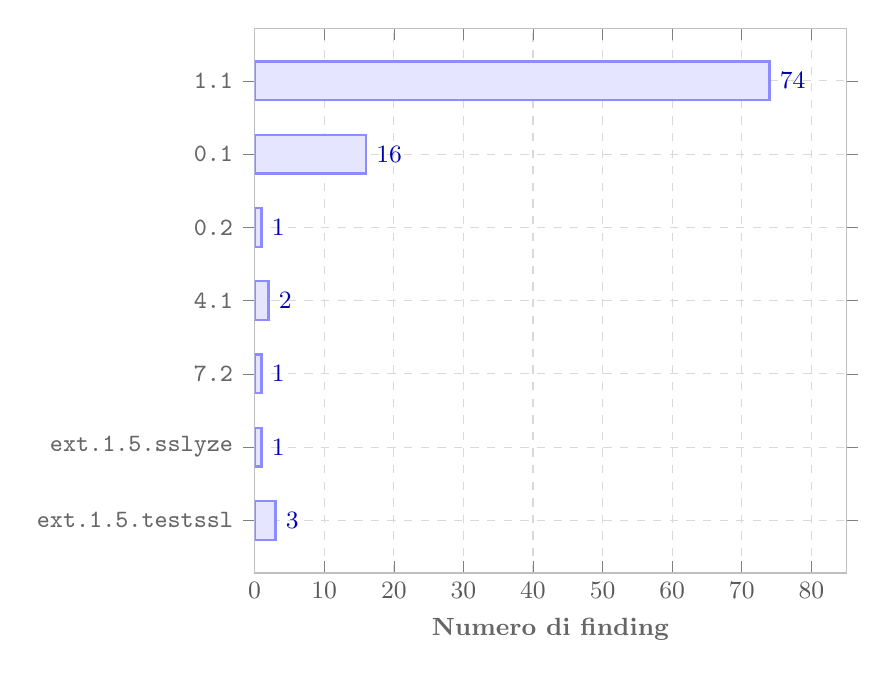
\begin{tikzpicture}
      \begin{axis}[
          xbar,
          width=0.75\textwidth, % <-- CORREZIONE: Lascia il 25% di spazio per le etichette laterali
          height=8.5cm,
          bar width=14pt,
          %
          % Setup Asse X
          xmin=0, xmax=85,
          xtick={0,10,20,30,40,50,60,70,80},
          xlabel={Numero di finding},
          xlabel style={font=\small\bfseries, text=gray!80!black},
          tick label style={font=\small, text=gray!70!black},
          %
          % Setup Asse Y
          symbolic y coords={{ext.1.5.testssl},{ext.1.5.sslyze},{7.2},{4.1},{0.2},{0.1},{1.1}},
          ytick=data,
          yticklabel style={font=\small\ttfamily, text=gray!80!black},
          enlarge y limits=0.12,
          %
          % Griglia
          grid=major,
          grid style={dashed, gray!30},
          axis line style={gray!50},
          %
          % Numeri a fianco delle barre
          nodes near coords,
          nodes near coords align={horizontal},
          every node near coord/.style={font=\small\bfseries, text=blue!70!black},
        ]

        \addplot[fill=blue!10, draw=blue!45, thick] coordinates {
            (3,{ext.1.5.testssl})
            (1,{ext.1.5.sslyze})
            (1,{7.2})
            (2,{4.1})
            (1,{0.2})
            (16,{0.1})
            (74,{1.1})
          };
      \end{axis}
    \end{tikzpicture}
  \end{adjustbox}
  \caption{Distribuzione dei 98 finding per test nell'assessment di validazione.}
  \label{fig:finding-distribution}
\end{figure}

\noindent{\small Cap.~5, §5.3, [DISCUTI] distribuzione 98 finding per test. Verificare ridondanza con tab:risultati-per-test.}
\clearpage

% ── Cap. 6 ───────────────────────────────────────────────────────────────────

% INSERIRE
% Cap. 6, §6.2.1
%
% PRIMA   : "Con codici semanticamente distinti questo routing è automatizzabile senza leggere i log."
% DOPO    : "Sistemi di \gls{CI/CD} come GitHub Actions o GitLab \gls{CI}"
% REF     : modifica frase esistente:
%   PRIMA "Con codici semanticamente distinti questo routing è automatizzabile senza leggere i log."
%   DOPO  "Con codici semanticamente distinti questo routing è automatizzabile senza leggere i log, come schematizzato nella Figura~\ref{fig:cicd-decision-tree}."
\begin{figure}[htbp]
  \centering
  \begin{adjustbox}{max width=\textwidth}
    \begin{tikzpicture}[
        % Stili Gold Standard (niente dipendenze da classi esterne)
        base/.style={draw, rounded corners=1pt, inner sep=6pt, align=center, font=\small, minimum height=3.5ex},
        cmd/.style={base, fill=blue!5, draw=blue!40, font=\small\ttfamily, minimum width=16em},
        decision/.style={draw, shape=diamond, aspect=2.5, inner sep=2pt, align=center, font=\small, fill=orange!10, draw=orange!50},
        %
        % Stili per gli Exit Codes (Larghezza fissa per allineamento a colonna)
        code0/.style={base, fill=green!10, draw=green!50!black, minimum width=8.5em},
        code1/.style={base, fill=red!10, draw=red!60!black, minimum width=8.5em},
        code2/.style={base, fill=orange!10, draw=orange!60!black, minimum width=8.5em},
        code10/.style={base, fill=gray!15, draw=gray!60!black, minimum width=8.5em},
        %
        % Stili per le Actions (Larghezza fissa e generosa)
        act0/.style={base, fill=green!5, draw=green!40, minimum width=13em},
        act1/.style={base, fill=red!5, draw=red!40, minimum width=13em},
        act2/.style={base, fill=orange!5, draw=orange!40, minimum width=13em},
        act10/.style={base, fill=gray!5, draw=gray!40, minimum width=13em},
      ]

      %% ── Asse Centrale (Runner -> Comando -> Decisione) ────────────────────
      \node[base, fill=gray!10, draw=gray!40, font=\small\bfseries] (start) {Runner CI/CD};
      \node[cmd, below=3ex of start] (cmd) {apiguard run -{}-config config.yaml};
      \node[decision, below=3ex of cmd] (dec) {exit code?};

      %% ── Colonna Exit Codes (Ancorati in alto a sx, coordinate forzate) ────
      % Il primo è spostato a destra di 4em rispetto al centro del rombo
      \path (dec.south) ++(4em, -4ex) node[code0, anchor=north west] (e0) {\textbf{\texttt{0}: CLEAN}\\{\scriptsize tutti PASS/SKIP}};
      \path (e0.south west) ++(0, -2.5ex) node[code1, anchor=north west] (e1) {\textbf{\texttt{1}: FAIL}\\{\scriptsize almeno un FAIL}};
      \path (e1.south west) ++(0, -2.5ex) node[code2, anchor=north west] (e2) {\textbf{\texttt{2}: ERROR}\\{\scriptsize ERROR senza FAIL}};
      \path (e2.south west) ++(0, -2.5ex) node[code10, anchor=north west] (e10) {\textbf{\texttt{10}: INFRA}\\{\scriptsize errore infrastrutturale}};

      %% ── Colonna Actions (Ancorate esattamente a 3em a destra dei codici) ──
      \path (e0.east) ++(3em, 0) node[act0, anchor=west] (a0) {\textbf{Pipeline prosegue}\\{\scriptsize (merge / deploy consentito)}};
      \path (e1.east) ++(3em, 0) node[act1, anchor=west] (a1) {\textbf{Blocco merge/deploy}\\{\scriptsize Report allegato come artefatto}};
      \path (e2.east) ++(3em, 0) node[act2, anchor=west] (a2) {\textbf{Alert malfunzionamento}\\{\scriptsize Revisione manuale richiesta}};
      \path (e10.east) ++(3em, 0) node[act10, anchor=west] (a10) {\textbf{Diagnosi deployment}\\{\scriptsize Verifica \texttt{config.yaml}}};

      %% ── Frecce di Flusso Principale ───────────────────────────────────────
      % Uso -latex per garantire la punta della freccia pulita senza dipendere da ag-arr
      \draw[-latex, semithick] (start) -- (cmd);
      \draw[-latex, semithick] (cmd) -- (dec);

      %% ── Routing a Bus per le condizioni (Il tronco verticale) ─────────────
      \coordinate (bus-end) at (dec.south |- e10.west);
      \draw[gray!70, semithick] (dec.south) -- (bus-end);

      % Diramazioni orizzontali verso gli Exit Code (colorate)
      \draw[-latex, semithick, green!50!black] (dec.south |- e0.west) -- (e0.west);
      \fill[gray!70] (dec.south |- e0.west) circle (1.5pt);

      \draw[-latex, semithick, red!60!black] (dec.south |- e1.west) -- (e1.west);
      \fill[gray!70] (dec.south |- e1.west) circle (1.5pt);

      \draw[-latex, semithick, orange!60!black] (dec.south |- e2.west) -- (e2.west);
      \fill[gray!70] (dec.south |- e2.west) circle (1.5pt);

      \draw[-latex, semithick, gray!60!black] (dec.south |- e10.west) -- (e10.west);
      \fill[gray!70] (dec.south |- e10.west) circle (1.5pt);

      %% ── Frecce dalle Condizioni alle Azioni (colorate in scala) ───────────
      \draw[-latex, semithick, green!50!black] (e0.east) -- (a0.west);
      \draw[-latex, semithick, red!60!black] (e1.east) -- (a1.west);
      \draw[-latex, semithick, orange!60!black] (e2.east) -- (a2.west);
      \draw[-latex, semithick, gray!60!black] (e10.east) -- (a10.west);

    \end{tikzpicture}
  \end{adjustbox}
  \caption{Routing degli exit code semantici (D6.P1) nella pipeline \gls{CI/CD}.}
  \label{fig:cicd-decision-tree}
\end{figure}

\noindent{\small Cap.~6, §6.2.1, routing exit code semantici (D6.P1): 0 clean, 1 fail, 2 error, 10 infra.}
\clearpage

% INSERIRE
% Cap. 6, §6.3.2
%
% PRIMA   : "garantendo che i finding prodotti da moduli distinti siano confrontabili nel report finale."
% DOPO    : "\paragraph{Coverage augmentation progressiva.}"
% REF     : aggiungere frase nel corpo del paragrafo prima della figura: La Figura~\ref{fig:modular-platform} illustra l'architettura a stella risultante, con il core invariato e i moduli di protocollo come unità intercambiabili.
\begin{figure}[htbp]
  \centering
  \begin{adjustbox}{max width=\textwidth}
    \begin{tikzpicture}[
        % Distanze calibrate
        node distance=4.5ex and 2.5em,
        %
        % Stili di base
        base/.style={draw, rounded corners=2pt, inner sep=8pt, align=center, font=\small},
        %
        % Core invariante leggermente allargato a 22em per accogliere la nuova riga dei contratti
        core/.style={base, fill=blue!8, draw=blue!45, minimum width=22em, thick},
        % Plugin mantenuto proporzionale (2em in meno del core)
        active/.style={base, fill=green!10, draw=green!50!black, minimum width=20em},
        %
        % Moduli Satelliti
        planned/.style={base, fill=gray!4, draw=gray!40, dashed, minimum width=8em},
        %
        % Stili Frecce
        arr-active/.style={-latex, thick, green!50!black},
        arr-planned/.style={-latex, thick, dashed, gray!50}
      ]

      %% ── Core immutabile (Centro) ──────────────────────────────────────────
      \node[core] (core) {
      \textbf{Core: infrastruttura immutabile}\\[1.5ex]
      {\footnotesize \texttt{Engine} \textbar{} \texttt{DAGScheduler} \textbar{} \texttt{EvidenceStore}}\\[0.8ex]
      {\footnotesize \texttt{TestContext} \textbar{} \texttt{TargetContext}}\\[0.8ex]
      {\footnotesize \texttt{BaseTest} \textbar{} \texttt{BaseConnector} \textbar{} \texttt{BaseGatewayAdapter}}\\[0.8ex]
      {\footnotesize \texttt{TestResult} \textbar{} \texttt{Finding} \textbar{} \texttt{EvidenceRecord}}
      };

      %% ── Moduli Satelliti (A stella) ───────────────────────────────────────
      % Modulo attivo (Sopra)
      \node[active, above=of core] (rest) {
      \textbf{Plugin REST (\gls{OAS})} \ {\footnotesize\itshape (attivo)}\\[1.5ex]
      {\footnotesize \texttt{OpenAPI discovery} \textbar{} \texttt{AttackSurface}}\\[0.8ex]
      {\footnotesize \texttt{SecurityClient} \textbar{} \texttt{KongGatewayAdapter}}\\[0.8ex]
      {\footnotesize 18 Test nativi (Domini D0--D7)}
      };

      % Moduli pianificati (Destra, Sotto, Sinistra)
      \node[planned, right=of core] (gql) {\textbf{GraphQL}\\[0.5ex]{\footnotesize\itshape (pianificato)}};
      \node[planned, below=of core] (grpc) {\textbf{gRPC}\\[0.5ex]{\footnotesize\itshape (pianificato)}};
      \node[planned, left=of core] (ws) {\textbf{WebSocket}\\[0.5ex]{\footnotesize\itshape (pianificato)}};

      %% ── Frecce di Collegamento (Convergenti verso il Core) ────────────────
      \draw[arr-active] (rest.south) -- (core.north);
      \draw[arr-planned] (gql.west) -- (core.east);
      \draw[arr-planned] (grpc.north) -- (core.south);
      \draw[arr-planned] (ws.east) -- (core.west);

      %% ── Legenda e Note ────────────────────────────────────────────────────
      \node[font=\footnotesize, text=gray!80!black, below=4ex of grpc, align=center] (note) {
      frecce continue: modulo attivo \quad frecce tratteggiate: moduli pianificati\\[1ex]
      {\itshape Il discovery dinamico via \texttt{pkgutil} permette il caricamento trasparente di moduli di terze parti}
      };

    \end{tikzpicture}
  \end{adjustbox}
  \caption{Evoluzione di APIGuard Assurance verso una piattaforma modulare: separazione netta tra il core invariante e i plugin di protocollo.}
  \label{fig:modular-platform}
\end{figure}
\noindent{\small Cap.~6, §6.3.2, piattaforma modulare: core immutabile + moduli REST/GraphQL/gRPC/WebSocket.}
\clearpage